% Options for packages loaded elsewhere
\PassOptionsToPackage{unicode}{hyperref}
\PassOptionsToPackage{hyphens}{url}
\PassOptionsToPackage{dvipsnames,svgnames,x11names}{xcolor}
%
\documentclass[
  letterpaper,
  DIV=11,
  numbers=noendperiod]{scrartcl}

\usepackage{amsmath,amssymb}
\usepackage{iftex}
\ifPDFTeX
  \usepackage[T1]{fontenc}
  \usepackage[utf8]{inputenc}
  \usepackage{textcomp} % provide euro and other symbols
\else % if luatex or xetex
  \usepackage{unicode-math}
  \defaultfontfeatures{Scale=MatchLowercase}
  \defaultfontfeatures[\rmfamily]{Ligatures=TeX,Scale=1}
\fi
\usepackage{lmodern}
\ifPDFTeX\else  
    % xetex/luatex font selection
\fi
% Use upquote if available, for straight quotes in verbatim environments
\IfFileExists{upquote.sty}{\usepackage{upquote}}{}
\IfFileExists{microtype.sty}{% use microtype if available
  \usepackage[]{microtype}
  \UseMicrotypeSet[protrusion]{basicmath} % disable protrusion for tt fonts
}{}
\makeatletter
\@ifundefined{KOMAClassName}{% if non-KOMA class
  \IfFileExists{parskip.sty}{%
    \usepackage{parskip}
  }{% else
    \setlength{\parindent}{0pt}
    \setlength{\parskip}{6pt plus 2pt minus 1pt}}
}{% if KOMA class
  \KOMAoptions{parskip=half}}
\makeatother
\usepackage{xcolor}
\setlength{\emergencystretch}{3em} % prevent overfull lines
\setcounter{secnumdepth}{5}
% Make \paragraph and \subparagraph free-standing
\makeatletter
\ifx\paragraph\undefined\else
  \let\oldparagraph\paragraph
  \renewcommand{\paragraph}{
    \@ifstar
      \xxxParagraphStar
      \xxxParagraphNoStar
  }
  \newcommand{\xxxParagraphStar}[1]{\oldparagraph*{#1}\mbox{}}
  \newcommand{\xxxParagraphNoStar}[1]{\oldparagraph{#1}\mbox{}}
\fi
\ifx\subparagraph\undefined\else
  \let\oldsubparagraph\subparagraph
  \renewcommand{\subparagraph}{
    \@ifstar
      \xxxSubParagraphStar
      \xxxSubParagraphNoStar
  }
  \newcommand{\xxxSubParagraphStar}[1]{\oldsubparagraph*{#1}\mbox{}}
  \newcommand{\xxxSubParagraphNoStar}[1]{\oldsubparagraph{#1}\mbox{}}
\fi
\makeatother

\usepackage{color}
\usepackage{fancyvrb}
\newcommand{\VerbBar}{|}
\newcommand{\VERB}{\Verb[commandchars=\\\{\}]}
\DefineVerbatimEnvironment{Highlighting}{Verbatim}{commandchars=\\\{\}}
% Add ',fontsize=\small' for more characters per line
\usepackage{framed}
\definecolor{shadecolor}{RGB}{241,243,245}
\newenvironment{Shaded}{\begin{snugshade}}{\end{snugshade}}
\newcommand{\AlertTok}[1]{\textcolor[rgb]{0.68,0.00,0.00}{#1}}
\newcommand{\AnnotationTok}[1]{\textcolor[rgb]{0.37,0.37,0.37}{#1}}
\newcommand{\AttributeTok}[1]{\textcolor[rgb]{0.40,0.45,0.13}{#1}}
\newcommand{\BaseNTok}[1]{\textcolor[rgb]{0.68,0.00,0.00}{#1}}
\newcommand{\BuiltInTok}[1]{\textcolor[rgb]{0.00,0.23,0.31}{#1}}
\newcommand{\CharTok}[1]{\textcolor[rgb]{0.13,0.47,0.30}{#1}}
\newcommand{\CommentTok}[1]{\textcolor[rgb]{0.37,0.37,0.37}{#1}}
\newcommand{\CommentVarTok}[1]{\textcolor[rgb]{0.37,0.37,0.37}{\textit{#1}}}
\newcommand{\ConstantTok}[1]{\textcolor[rgb]{0.56,0.35,0.01}{#1}}
\newcommand{\ControlFlowTok}[1]{\textcolor[rgb]{0.00,0.23,0.31}{\textbf{#1}}}
\newcommand{\DataTypeTok}[1]{\textcolor[rgb]{0.68,0.00,0.00}{#1}}
\newcommand{\DecValTok}[1]{\textcolor[rgb]{0.68,0.00,0.00}{#1}}
\newcommand{\DocumentationTok}[1]{\textcolor[rgb]{0.37,0.37,0.37}{\textit{#1}}}
\newcommand{\ErrorTok}[1]{\textcolor[rgb]{0.68,0.00,0.00}{#1}}
\newcommand{\ExtensionTok}[1]{\textcolor[rgb]{0.00,0.23,0.31}{#1}}
\newcommand{\FloatTok}[1]{\textcolor[rgb]{0.68,0.00,0.00}{#1}}
\newcommand{\FunctionTok}[1]{\textcolor[rgb]{0.28,0.35,0.67}{#1}}
\newcommand{\ImportTok}[1]{\textcolor[rgb]{0.00,0.46,0.62}{#1}}
\newcommand{\InformationTok}[1]{\textcolor[rgb]{0.37,0.37,0.37}{#1}}
\newcommand{\KeywordTok}[1]{\textcolor[rgb]{0.00,0.23,0.31}{\textbf{#1}}}
\newcommand{\NormalTok}[1]{\textcolor[rgb]{0.00,0.23,0.31}{#1}}
\newcommand{\OperatorTok}[1]{\textcolor[rgb]{0.37,0.37,0.37}{#1}}
\newcommand{\OtherTok}[1]{\textcolor[rgb]{0.00,0.23,0.31}{#1}}
\newcommand{\PreprocessorTok}[1]{\textcolor[rgb]{0.68,0.00,0.00}{#1}}
\newcommand{\RegionMarkerTok}[1]{\textcolor[rgb]{0.00,0.23,0.31}{#1}}
\newcommand{\SpecialCharTok}[1]{\textcolor[rgb]{0.37,0.37,0.37}{#1}}
\newcommand{\SpecialStringTok}[1]{\textcolor[rgb]{0.13,0.47,0.30}{#1}}
\newcommand{\StringTok}[1]{\textcolor[rgb]{0.13,0.47,0.30}{#1}}
\newcommand{\VariableTok}[1]{\textcolor[rgb]{0.07,0.07,0.07}{#1}}
\newcommand{\VerbatimStringTok}[1]{\textcolor[rgb]{0.13,0.47,0.30}{#1}}
\newcommand{\WarningTok}[1]{\textcolor[rgb]{0.37,0.37,0.37}{\textit{#1}}}

\providecommand{\tightlist}{%
  \setlength{\itemsep}{0pt}\setlength{\parskip}{0pt}}\usepackage{longtable,booktabs,array}
\usepackage{calc} % for calculating minipage widths
% Correct order of tables after \paragraph or \subparagraph
\usepackage{etoolbox}
\makeatletter
\patchcmd\longtable{\par}{\if@noskipsec\mbox{}\fi\par}{}{}
\makeatother
% Allow footnotes in longtable head/foot
\IfFileExists{footnotehyper.sty}{\usepackage{footnotehyper}}{\usepackage{footnote}}
\makesavenoteenv{longtable}
\usepackage{graphicx}
\makeatletter
\newsavebox\pandoc@box
\newcommand*\pandocbounded[1]{% scales image to fit in text height/width
  \sbox\pandoc@box{#1}%
  \Gscale@div\@tempa{\textheight}{\dimexpr\ht\pandoc@box+\dp\pandoc@box\relax}%
  \Gscale@div\@tempb{\linewidth}{\wd\pandoc@box}%
  \ifdim\@tempb\p@<\@tempa\p@\let\@tempa\@tempb\fi% select the smaller of both
  \ifdim\@tempa\p@<\p@\scalebox{\@tempa}{\usebox\pandoc@box}%
  \else\usebox{\pandoc@box}%
  \fi%
}
% Set default figure placement to htbp
\def\fps@figure{htbp}
\makeatother

\KOMAoption{captions}{tableheading}
\makeatletter
\@ifpackageloaded{caption}{}{\usepackage{caption}}
\AtBeginDocument{%
\ifdefined\contentsname
  \renewcommand*\contentsname{Table of contents}
\else
  \newcommand\contentsname{Table of contents}
\fi
\ifdefined\listfigurename
  \renewcommand*\listfigurename{List of Figures}
\else
  \newcommand\listfigurename{List of Figures}
\fi
\ifdefined\listtablename
  \renewcommand*\listtablename{List of Tables}
\else
  \newcommand\listtablename{List of Tables}
\fi
\ifdefined\figurename
  \renewcommand*\figurename{Figure}
\else
  \newcommand\figurename{Figure}
\fi
\ifdefined\tablename
  \renewcommand*\tablename{Table}
\else
  \newcommand\tablename{Table}
\fi
}
\@ifpackageloaded{float}{}{\usepackage{float}}
\floatstyle{ruled}
\@ifundefined{c@chapter}{\newfloat{codelisting}{h}{lop}}{\newfloat{codelisting}{h}{lop}[chapter]}
\floatname{codelisting}{Listing}
\newcommand*\listoflistings{\listof{codelisting}{List of Listings}}
\makeatother
\makeatletter
\makeatother
\makeatletter
\@ifpackageloaded{caption}{}{\usepackage{caption}}
\@ifpackageloaded{subcaption}{}{\usepackage{subcaption}}
\makeatother

\usepackage{bookmark}

\IfFileExists{xurl.sty}{\usepackage{xurl}}{} % add URL line breaks if available
\urlstyle{same} % disable monospaced font for URLs
\hypersetup{
  pdftitle={Machine Learning I},
  pdfauthor={Dante Conti, Sergi Ramirez, (c) IDEAI},
  colorlinks=true,
  linkcolor={blue},
  filecolor={Maroon},
  citecolor={Blue},
  urlcolor={Blue},
  pdfcreator={LaTeX via pandoc}}


\title{Machine Learning I}
\usepackage{etoolbox}
\makeatletter
\providecommand{\subtitle}[1]{% add subtitle to \maketitle
  \apptocmd{\@title}{\par {\large #1 \par}}{}{}
}
\makeatother
\subtitle{KNN y Naives Bayes}
\author{Dante Conti, Sergi Ramirez, (c) IDEAI}
\date{2025-10-14}

\begin{document}
\maketitle

\renewcommand*\contentsname{Table of contents}
{
\hypersetup{linkcolor=}
\setcounter{tocdepth}{3}
\tableofcontents
}

\subsection{Definición del problema}\label{definiciuxf3n-del-problema}

\subsubsection{Contexto}\label{contexto}

Una tienda está planteando la venta final del año. Queremos lanzar una
oferta. Será válido sólo para los clientes existentes y la campaña a
través de las llamadas telefónicas que se está planificando actualmente
para ellos. La dirección considera que la mejor manera de reducir el
coste de la campaña es hacer un modelo predictivo que clasifique a los
clientes que puedan comprar la oferta.

Las variables que contiene la base de datos son:

\begin{itemize}
\tightlist
\item
  \textbf{Response (target)}: 1 si el cliente aceptó la oferta en la
  última campaña, 0 en caso contrario
\item
  \textbf{ID}: ID único de cada cliente
\item
  \textbf{Year\_Birth} - Edad del cliente
\item
  \textbf{Complain} - 1 si el cliente presentó una queja en los últimos
  2 años
\item
  \textbf{Dt\_Customer} - Fecha de alta del cliente en la empresa
\item
  \textbf{Education} - Nivel de estudios del cliente
\item
  \textbf{Marital} - Estado civil del cliente
\item
  \textbf{Kidhome} - Número de niños pequeños en el hogar del cliente
\item
  \textbf{Teenhome} - Número de adolescentes en el hogar del cliente
\item
  \textbf{Income} - Ingresos anuales del hogar del cliente
\item
  \textbf{MntFishProducts} - Cantidad gastada en productos de pescado en
  los últimos 2 años
\item
  \textbf{MntMeatProducts} - Cantidad gastada en productos cárnicos en
  los últimos 2 años
\item
  \textbf{MntFruits} - Cantidad gastada en frutas en los últimos 2 años
\item
  \textbf{MntSweetProducts} - cantidad gastada en productos dulces en
  los últimos 2 años
\item
  \textbf{MntWines} - cantidad gastada en productos de vino en los
  últimos 2 años
\item
  \textbf{MntGoldProds} - cantidad gastada en productos de oro en los
  últimos 2 años
\item
  \textbf{NumDealsPurchases} - número de compras realizadas con
  descuento
\item
  \textbf{NumCatalogPurchases} - número de compras realizadas por
  catálogo (comprando productos con envío por correo)
\item
  \textbf{NumStorePurchases} - número de compras realizadas directamente
  en tiendas
\item
  \textbf{NumWebPurchases} - número de compras realizadas a través del
  sitio web de la empresa
\item
  \textbf{NumWebVisitsMonth} - número de visitas al sitio web de la
  empresa en el último mes
\item
  \textbf{Recency} - número de días desde la última compra
\end{itemize}

\subsubsection{Objetivo}\label{objetivo}

Ls supertienda quiere predecir la probabilidad que el cliente de una
respuesta positiva y identificar los diferentes factores que afectan la
respuesta del cliente.

Podéis encontrar la base de datos en la siguiente
\href{https://www.kaggle.com/datasets/ahsan81/superstore-marketing-campaign-dataset}{web}

\begin{verbatim}
  Income Kidhome Teenhome Recency MntWines MntFruits MntMeatProducts
1  84835       0        0       0      189       104             379
2  57091       0        0       0      464         5              64
3  67267       0        1       0      134        11              59
4  32474       1        1       0       10         0               1
5  21474       1        0       0        6        16              24
6  71691       0        0       0      336       130             411
  MntFishProducts MntSweetProducts MntGoldProds NumDealsPurchases
1             111              189          218                 1
2               7                0           37                 1
3              15                2           30                 1
4               0                0            0                 1
5              11                0           34                 2
6             240               32           43                 1
  NumWebPurchases NumCatalogPurchases NumStorePurchases NumWebVisitsMonth
1               4                   4                 6                 1
2               7                   3                 7                 5
3               3                   2                 5                 2
4               1                   0                 2                 7
5               3                   1                 2                 7
6               4                   7                 5                 2
  Response Edad Education_Basic Education_Graduation Education_Master
1      Yes   55               0                    1                0
2      Yes   64               0                    1                0
3       No   67               0                    1                0
4       No   58               0                    1                0
5      Yes   36               0                    1                0
6      Yes   67               0                    0                0
  Education_PhD Marital_Status_Alone Marital_Status_Divorced
1             0                    0                       1
2             0                    0                       0
3             0                    0                       0
4             0                    0                       0
5             0                    0                       0
6             1                    0                       0
  Marital_Status_Married Marital_Status_Single Marital_Status_Together
1                      0                     0                       0
2                      0                     1                       0
3                      1                     0                       0
4                      0                     0                       1
5                      0                     1                       0
6                      0                     1                       0
  Marital_Status_Widow Marital_Status_YOLO mes_cliente_2 mes_cliente_3
1                    0                   0             0             0
2                    0                   0             0             0
3                    0                   0             0             0
4                    0                   0             0             0
5                    0                   0             0             0
6                    0                   0             0             1
  mes_cliente_4 mes_cliente_5 mes_cliente_6 mes_cliente_7 mes_cliente_8
1             0             0             1             0             0
2             0             0             1             0             0
3             0             1             0             0             0
4             0             0             0             0             0
5             0             0             0             0             1
6             0             0             0             0             0
  mes_cliente_9 mes_cliente_10 mes_cliente_11 mes_cliente_12 Complain_Yes
1             0              0              0              0            0
2             0              0              0              0            0
3             0              0              0              0            0
4             0              0              1              0            0
5             0              0              0              0            0
6             0              0              0              0            0
\end{verbatim}

\subsection{KNN}\label{knn}

\subsubsection{KNN Classifier}\label{knn-classifier}

\paragraph{Definimos los conjuntos de
datos}\label{definimos-los-conjuntos-de-datos}

\subsection{R: R Base}

\begin{Shaded}
\begin{Highlighting}[]
\FunctionTok{set.seed}\NormalTok{(}\DecValTok{1994}\NormalTok{)}

\NormalTok{ind\_col }\OtherTok{\textless{}{-}} \FunctionTok{c}\NormalTok{(}\DecValTok{16}\NormalTok{)}

\NormalTok{default\_idx }\OtherTok{=} \FunctionTok{sample}\NormalTok{(}\FunctionTok{nrow}\NormalTok{(datos), }\FunctionTok{nrow}\NormalTok{(datos)}\SpecialCharTok{*}\FloatTok{0.7}\NormalTok{)}
\NormalTok{train }\OtherTok{\textless{}{-}}\NormalTok{ datos[default\_idx, ]; test }\OtherTok{\textless{}{-}}\NormalTok{ datos[}\SpecialCharTok{{-}}\NormalTok{default\_idx, ]}
\NormalTok{X\_train }\OtherTok{\textless{}{-}}\NormalTok{ train[, }\SpecialCharTok{{-}}\NormalTok{ind\_col]; X\_test }\OtherTok{\textless{}{-}}\NormalTok{ test[, }\SpecialCharTok{{-}}\NormalTok{ind\_col]}
\NormalTok{y\_train }\OtherTok{\textless{}{-}}\NormalTok{ train[, ind\_col]; y\_test }\OtherTok{\textless{}{-}}\NormalTok{ test[, ind\_col]}

\CommentTok{\# Convertimos todas las columnas en numéricas para que se pueda utilizar el algoritmo}
\CommentTok{\# de KNN}
\NormalTok{X\_train }\OtherTok{\textless{}{-}} \FunctionTok{data.frame}\NormalTok{(}\FunctionTok{lapply}\NormalTok{(X\_train, as.numeric))}
\NormalTok{X\_test }\OtherTok{\textless{}{-}} \FunctionTok{data.frame}\NormalTok{(}\FunctionTok{lapply}\NormalTok{(X\_test, as.numeric))}
\end{Highlighting}
\end{Shaded}

\subsection{\texorpdfstring{R: Packages
\texttt{caret}}{R: Packages caret}}

\begin{Shaded}
\begin{Highlighting}[]
\FunctionTok{library}\NormalTok{(caret)}

\FunctionTok{set.seed}\NormalTok{(}\DecValTok{1994}\NormalTok{)}

\NormalTok{ind\_col }\OtherTok{\textless{}{-}} \FunctionTok{c}\NormalTok{(}\DecValTok{16}\NormalTok{)}
\NormalTok{default\_idx }\OtherTok{\textless{}{-}} \FunctionTok{createDataPartition}\NormalTok{(datos}\SpecialCharTok{$}\NormalTok{Response, }\AttributeTok{p =} \FloatTok{0.7}\NormalTok{, }\AttributeTok{list =} \ConstantTok{FALSE}\NormalTok{)}
\NormalTok{X\_trainC }\OtherTok{\textless{}{-}}\NormalTok{ datos[default\_idx, ]}
\NormalTok{X\_testC }\OtherTok{\textless{}{-}}\NormalTok{ datos[}\SpecialCharTok{{-}}\NormalTok{default\_idx, ]}
\NormalTok{y\_testC }\OtherTok{\textless{}{-}}\NormalTok{ X\_testC[, ind\_col]}
\NormalTok{X\_testC }\OtherTok{\textless{}{-}}\NormalTok{ X\_testC[, }\SpecialCharTok{{-}}\NormalTok{ind\_col]}
\end{Highlighting}
\end{Shaded}

\begin{Shaded}
\begin{Highlighting}[]
\FunctionTok{modelLookup}\NormalTok{(}\StringTok{"knn"}\NormalTok{)}
\end{Highlighting}
\end{Shaded}

\begin{verbatim}
  model parameter      label forReg forClass probModel
1   knn         k #Neighbors   TRUE     TRUE      TRUE
\end{verbatim}

\subsection{Python}

\begin{Shaded}
\begin{Highlighting}[]
\ImportTok{from}\NormalTok{ sklearn.model\_selection }\ImportTok{import}\NormalTok{ train\_test\_split}

\NormalTok{X }\OperatorTok{=}\NormalTok{ datos\_py.drop([}\StringTok{"Response"}\NormalTok{], axis}\OperatorTok{=}\DecValTok{1}\NormalTok{)}
\NormalTok{y }\OperatorTok{=}\NormalTok{ datos\_py[}\StringTok{\textquotesingle{}Response\textquotesingle{}}\NormalTok{]}

\NormalTok{X\_trainPy, X\_testPy, y\_trainPy, y\_testPy }\OperatorTok{=}\NormalTok{ train\_test\_split(X, y, test\_size }\OperatorTok{=} \FloatTok{0.3}\NormalTok{, random\_state }\OperatorTok{=} \DecValTok{1994}\NormalTok{)}
\end{Highlighting}
\end{Shaded}

\paragraph{Escalamos los datos}\label{escalamos-los-datos}

\subsection{R: R Base}

\begin{Shaded}
\begin{Highlighting}[]
\FunctionTok{library}\NormalTok{(scales)}

\CommentTok{\# Suponemos que X\_train y X\_test son data.frames numéricos}
\NormalTok{cols }\OtherTok{\textless{}{-}} \FunctionTok{colnames}\NormalTok{(X\_train)}

\CommentTok{\# Calcular medias y desviaciones estándar con X\_train}
\NormalTok{means }\OtherTok{\textless{}{-}} \FunctionTok{sapply}\NormalTok{(X\_train, mean)}
\NormalTok{sds }\OtherTok{\textless{}{-}} \FunctionTok{sapply}\NormalTok{(X\_train, sd)}

\CommentTok{\# Estandarizar X\_train}
\NormalTok{X\_train }\OtherTok{\textless{}{-}} \FunctionTok{scale}\NormalTok{(X\_train, }\AttributeTok{center =}\NormalTok{ means, }\AttributeTok{scale =}\NormalTok{ sds)}

\CommentTok{\# Aplicar la misma transformación a X\_test}
\NormalTok{X\_test }\OtherTok{\textless{}{-}} \FunctionTok{scale}\NormalTok{(X\_test, }\AttributeTok{center =}\NormalTok{ means, }\AttributeTok{scale =}\NormalTok{ sds)}

\CommentTok{\# Convertir de nuevo a data.frame}
\NormalTok{X\_train }\OtherTok{\textless{}{-}} \FunctionTok{as.data.frame}\NormalTok{(X\_train)}
\NormalTok{X\_test }\OtherTok{\textless{}{-}} \FunctionTok{as.data.frame}\NormalTok{(X\_test)}

\CommentTok{\# Mantener nombres de columnas}
\FunctionTok{colnames}\NormalTok{(X\_train) }\OtherTok{\textless{}{-}}\NormalTok{ cols}
\FunctionTok{colnames}\NormalTok{(X\_test) }\OtherTok{\textless{}{-}}\NormalTok{ cols}
\end{Highlighting}
\end{Shaded}

\subsection{\texorpdfstring{R: Packages
\texttt{caret}}{R: Packages caret}}

\begin{Shaded}
\begin{Highlighting}[]
\FunctionTok{library}\NormalTok{(caret)}

\CommentTok{\# Crear preprocesador para centrado y escalado}
\NormalTok{preproc }\OtherTok{\textless{}{-}} \FunctionTok{preProcess}\NormalTok{(X\_trainC, }\AttributeTok{method =} \FunctionTok{c}\NormalTok{(}\StringTok{"center"}\NormalTok{, }\StringTok{"scale"}\NormalTok{))}

\CommentTok{\# Aplicar transformación}
\NormalTok{X\_trainC }\OtherTok{\textless{}{-}} \FunctionTok{predict}\NormalTok{(preproc, X\_trainC)}
\NormalTok{X\_testC }\OtherTok{\textless{}{-}} \FunctionTok{predict}\NormalTok{(preproc, X\_testC)}
\end{Highlighting}
\end{Shaded}

\subsection{Python}

\begin{Shaded}
\begin{Highlighting}[]
\NormalTok{cols }\OperatorTok{=}\NormalTok{ X\_trainPy.columns}

\ImportTok{from}\NormalTok{ sklearn.preprocessing }\ImportTok{import}\NormalTok{ StandardScaler}
\ImportTok{import}\NormalTok{ pandas }\ImportTok{as}\NormalTok{ pd}

\NormalTok{scaler }\OperatorTok{=}\NormalTok{ StandardScaler()}
\NormalTok{X\_trainPy }\OperatorTok{=}\NormalTok{ scaler.fit\_transform(X\_trainPy)}
\NormalTok{X\_testPy }\OperatorTok{=}\NormalTok{ scaler.transform(X\_testPy)}

\NormalTok{X\_trainPy }\OperatorTok{=}\NormalTok{ pd.DataFrame(X\_trainPy, columns}\OperatorTok{=}\NormalTok{[cols])}
\NormalTok{X\_testPy }\OperatorTok{=}\NormalTok{ pd.DataFrame(X\_testPy, columns}\OperatorTok{=}\NormalTok{[cols])}
\end{Highlighting}
\end{Shaded}

\paragraph{Entrenamiento del modelo}\label{entrenamiento-del-modelo}

\subsection{R: R base}

\begin{Shaded}
\begin{Highlighting}[]
\NormalTok{prediccion }\OtherTok{\textless{}{-}} \FunctionTok{knn}\NormalTok{(}\AttributeTok{train =}\NormalTok{ X\_train, }\AttributeTok{test  =}\NormalTok{ X\_test, }\AttributeTok{cl =}\NormalTok{ y\_train, }\AttributeTok{k =} \DecValTok{3}\NormalTok{)}
\FunctionTok{head}\NormalTok{(prediccion)}
\end{Highlighting}
\end{Shaded}

\begin{verbatim}
[1] No  Yes No  No  No  Yes
Levels: No Yes
\end{verbatim}

\subsection{\texorpdfstring{R: Packages
\texttt{caret}}{R: Packages caret}}

\begin{Shaded}
\begin{Highlighting}[]
\NormalTok{(entrenamiento }\OtherTok{\textless{}{-}} \FunctionTok{train}\NormalTok{(Response }\SpecialCharTok{\textasciitilde{}}\NormalTok{ ., }\AttributeTok{data =}\NormalTok{ X\_trainC, }\AttributeTok{method =} \StringTok{"knn"}\NormalTok{,}
                        \AttributeTok{trControl =} \FunctionTok{trainControl}\NormalTok{(}\AttributeTok{method =} \StringTok{"cv"}\NormalTok{, }\AttributeTok{number =} \DecValTok{5}\NormalTok{),}
                        \CommentTok{\# preProcess = c("center", "scale"),}
                        \AttributeTok{tuneGrid =} \FunctionTok{expand.grid}\NormalTok{(}\AttributeTok{k =} \FunctionTok{seq}\NormalTok{(}\DecValTok{1}\NormalTok{, }\DecValTok{31}\NormalTok{, }\AttributeTok{by =} \DecValTok{2}\NormalTok{))))}
\end{Highlighting}
\end{Shaded}

\begin{verbatim}
k-Nearest Neighbors 

1553 samples
  39 predictor
   2 classes: 'No', 'Yes' 

No pre-processing
Resampling: Cross-Validated (5 fold) 
Summary of sample sizes: 1243, 1242, 1243, 1242, 1242 
Resampling results across tuning parameters:

  k   Accuracy   Kappa      
   1  0.8325879  0.279679994
   3  0.8473976  0.213133436
   5  0.8493185  0.131995536
   7  0.8544695  0.126768918
   9  0.8538347  0.110964792
  11  0.8493206  0.054785486
  13  0.8486796  0.032064246
  15  0.8467483  0.023317027
  17  0.8467524  0.006447460
  19  0.8473955  0.007760759
  21  0.8493289  0.011490079
  23  0.8480386  0.003353250
  25  0.8486817  0.004620608
  27  0.8493248  0.005851422
  29  0.8486796  0.004579949
  31  0.8493227  0.005847308

Accuracy was used to select the optimal model using the largest value.
The final value used for the model was k = 7.
\end{verbatim}

\begin{Shaded}
\begin{Highlighting}[]
\NormalTok{entrenamiento}\SpecialCharTok{$}\NormalTok{modelType}
\end{Highlighting}
\end{Shaded}

\begin{verbatim}
[1] "Classification"
\end{verbatim}

\subsection{Python}

\begin{Shaded}
\begin{Highlighting}[]
\CommentTok{\# import KNeighbors ClaSSifier from sklearn}
\ImportTok{from}\NormalTok{ sklearn.neighbors }\ImportTok{import}\NormalTok{ KNeighborsClassifier}

\CommentTok{\# instantiate the model}
\NormalTok{knn }\OperatorTok{=}\NormalTok{ KNeighborsClassifier(n\_neighbors }\OperatorTok{=} \DecValTok{3}\NormalTok{)}

\CommentTok{\# fit the model to the training set}
\NormalTok{knn.fit(X\_trainPy, y\_trainPy)}
\end{Highlighting}
\end{Shaded}

\begin{verbatim}
KNeighborsClassifier(n_neighbors=3)
\end{verbatim}

\paragraph{\texorpdfstring{\emph{Tunning parameters}: Selección del
valor de
k}{Tunning parameters: Selección del valor de k}}\label{tunning-parameters-selecciuxf3n-del-valor-de-k}

\subsection{R: R base}

\begin{Shaded}
\begin{Highlighting}[]
\FunctionTok{set.seed}\NormalTok{(}\DecValTok{42}\NormalTok{)}
\NormalTok{k\_to\_try }\OtherTok{=} \DecValTok{1}\SpecialCharTok{:}\DecValTok{100}
\NormalTok{err\_k }\OtherTok{=} \FunctionTok{rep}\NormalTok{(}\AttributeTok{x =} \DecValTok{0}\NormalTok{, }\AttributeTok{times =} \FunctionTok{length}\NormalTok{(k\_to\_try))}

\ControlFlowTok{for}\NormalTok{ (i }\ControlFlowTok{in} \FunctionTok{seq\_along}\NormalTok{(k\_to\_try)) \{}
\NormalTok{  pred }\OtherTok{\textless{}{-}} \FunctionTok{knn}\NormalTok{(}\AttributeTok{train =}\NormalTok{ X\_train, }
             \AttributeTok{test  =}\NormalTok{ X\_test, }
             \AttributeTok{cl    =}\NormalTok{ y\_train, }
             \AttributeTok{k     =}\NormalTok{ k\_to\_try[i], }
             \AttributeTok{prob =}\NormalTok{ T)}
\NormalTok{  err\_k[i] }\OtherTok{\textless{}{-}} \FunctionTok{calc\_class\_err}\NormalTok{(y\_test, pred)}
\NormalTok{\}}
\end{Highlighting}
\end{Shaded}

\begin{Shaded}
\begin{Highlighting}[]
\CommentTok{\# plot error vs choice of k}
\FunctionTok{plot}\NormalTok{(err\_k, }\AttributeTok{type =} \StringTok{"b"}\NormalTok{, }\AttributeTok{col =} \StringTok{"dodgerblue"}\NormalTok{, }\AttributeTok{cex =} \DecValTok{1}\NormalTok{, }\AttributeTok{pch =} \DecValTok{20}\NormalTok{, }
     \AttributeTok{xlab =} \StringTok{"k, number of neighbors"}\NormalTok{, }\AttributeTok{ylab =} \StringTok{"classification error"}\NormalTok{,}
     \AttributeTok{main =} \StringTok{"(Test) Error Rate vs Neighbors"}\NormalTok{)}
\CommentTok{\# add line for min error seen}
\FunctionTok{abline}\NormalTok{(}\AttributeTok{h =} \FunctionTok{min}\NormalTok{(err\_k), }\AttributeTok{col =} \StringTok{"darkorange"}\NormalTok{, }\AttributeTok{lty =} \DecValTok{3}\NormalTok{)}
\CommentTok{\# add line for minority prevalence in test set}
\FunctionTok{abline}\NormalTok{(}\AttributeTok{h =} \FunctionTok{mean}\NormalTok{(y\_test }\SpecialCharTok{==} \StringTok{"Yes"}\NormalTok{), }\AttributeTok{col =} \StringTok{"grey"}\NormalTok{, }\AttributeTok{lty =} \DecValTok{2}\NormalTok{)}
\end{Highlighting}
\end{Shaded}

\pandocbounded{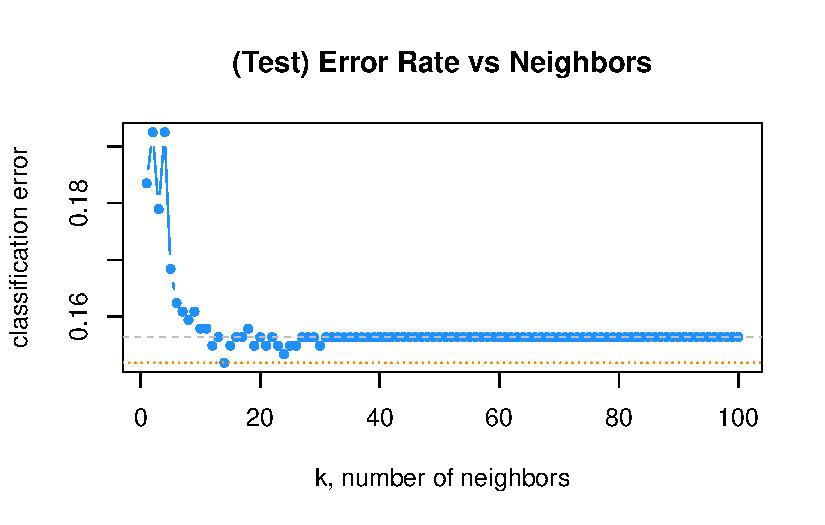
\includegraphics[keepaspectratio]{KnnNB_files/figure-pdf/visualizar_movimiento_base-1.pdf}}

\subsection{\texorpdfstring{R: Packages
\texttt{caret}}{R: Packages caret}}

\begin{Shaded}
\begin{Highlighting}[]
\NormalTok{get\_best\_result }\OtherTok{=} \ControlFlowTok{function}\NormalTok{(caret\_fit) \{}
\NormalTok{  best }\OtherTok{=} \FunctionTok{which}\NormalTok{(}\FunctionTok{rownames}\NormalTok{(caret\_fit}\SpecialCharTok{$}\NormalTok{results) }\SpecialCharTok{==} \FunctionTok{rownames}\NormalTok{(caret\_fit}\SpecialCharTok{$}\NormalTok{bestTune))}
\NormalTok{  best\_result }\OtherTok{=}\NormalTok{ caret\_fit}\SpecialCharTok{$}\NormalTok{results[best, ]}
  \FunctionTok{rownames}\NormalTok{(best\_result) }\OtherTok{=} \ConstantTok{NULL}
\NormalTok{  best\_result}
\NormalTok{\}}
\end{Highlighting}
\end{Shaded}

\begin{Shaded}
\begin{Highlighting}[]
\FunctionTok{head}\NormalTok{(entrenamiento}\SpecialCharTok{$}\NormalTok{results, }\DecValTok{5}\NormalTok{)}
\end{Highlighting}
\end{Shaded}

\begin{verbatim}
  k  Accuracy     Kappa  AccuracySD    KappaSD
1 1 0.8325879 0.2796800 0.012589167 0.04474886
2 3 0.8473976 0.2131334 0.015312908 0.09135524
3 5 0.8493185 0.1319955 0.014549182 0.10608590
4 7 0.8544695 0.1267689 0.007133587 0.06311837
5 9 0.8538347 0.1109648 0.007330331 0.05904349
\end{verbatim}

\begin{Shaded}
\begin{Highlighting}[]
\FunctionTok{plot}\NormalTok{(entrenamiento)}
\end{Highlighting}
\end{Shaded}

\pandocbounded{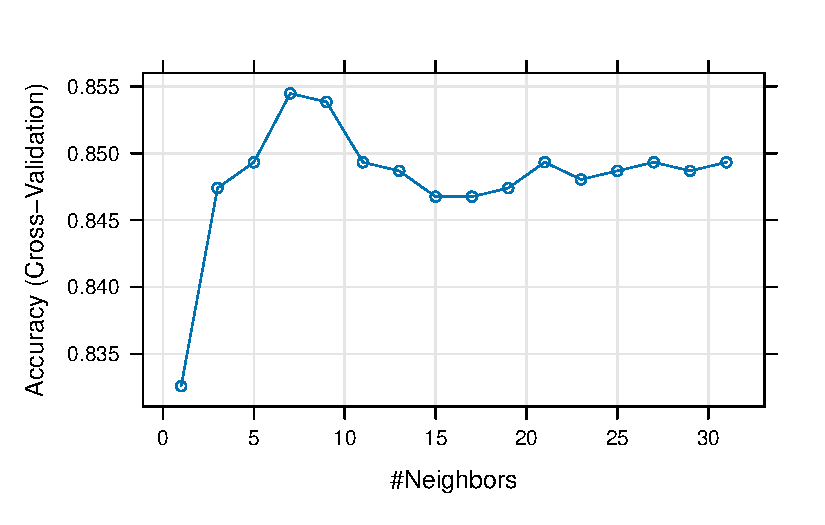
\includegraphics[keepaspectratio]{KnnNB_files/figure-pdf/grafico_accuracy_caret-1.pdf}}

\begin{Shaded}
\begin{Highlighting}[]
\NormalTok{tablaResultados }\OtherTok{\textless{}{-}}\NormalTok{ entrenamiento}\SpecialCharTok{$}\NormalTok{results}
\NormalTok{tablaResultados}\SpecialCharTok{$}\NormalTok{error }\OtherTok{\textless{}{-}} \DecValTok{1} \SpecialCharTok{{-}}\NormalTok{ tablaResultados}\SpecialCharTok{$}\NormalTok{Accuracy}

\CommentTok{\# plot error vs choice of k}
\FunctionTok{plot}\NormalTok{(tablaResultados}\SpecialCharTok{$}\NormalTok{error, }\AttributeTok{type =} \StringTok{"b"}\NormalTok{, }\AttributeTok{col =} \StringTok{"dodgerblue"}\NormalTok{, }\AttributeTok{cex =} \DecValTok{1}\NormalTok{, }\AttributeTok{pch =} \DecValTok{20}\NormalTok{, }
     \AttributeTok{xlab =} \StringTok{"k, number of neighbors"}\NormalTok{, }\AttributeTok{ylab =} \StringTok{"classification error"}\NormalTok{,}
     \AttributeTok{main =} \StringTok{"(Test) Error Rate vs Neighbors"}\NormalTok{)}
\CommentTok{\# add line for min error seen}
\FunctionTok{abline}\NormalTok{(}\AttributeTok{h =} \FunctionTok{min}\NormalTok{(err\_k), }\AttributeTok{col =} \StringTok{"darkorange"}\NormalTok{, }\AttributeTok{lty =} \DecValTok{3}\NormalTok{)}
\CommentTok{\# add line for minority prevalence in test set}
\FunctionTok{abline}\NormalTok{(}\AttributeTok{h =} \FunctionTok{mean}\NormalTok{(y\_test }\SpecialCharTok{==} \StringTok{"Yes"}\NormalTok{), }\AttributeTok{col =} \StringTok{"grey"}\NormalTok{, }\AttributeTok{lty =} \DecValTok{2}\NormalTok{)}
\end{Highlighting}
\end{Shaded}

\pandocbounded{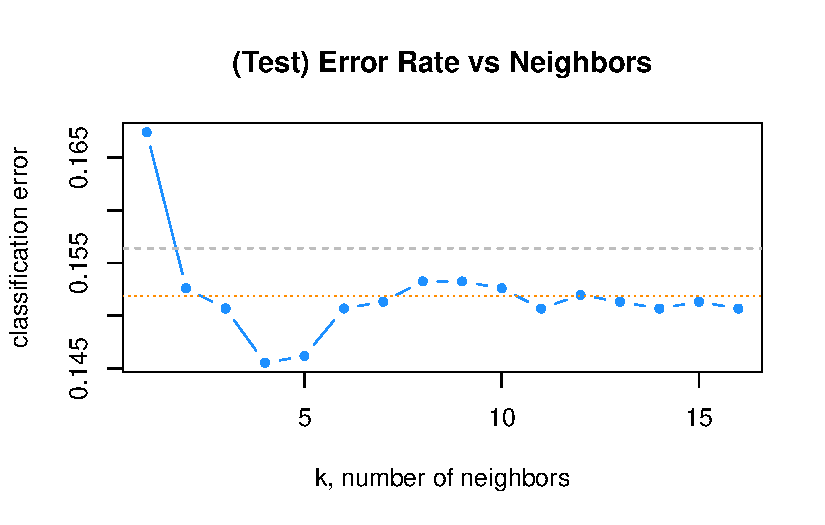
\includegraphics[keepaspectratio]{KnnNB_files/figure-pdf/grafico_accuracy_caret-2.pdf}}

\begin{Shaded}
\begin{Highlighting}[]
\FunctionTok{get\_best\_result}\NormalTok{(entrenamiento)}
\end{Highlighting}
\end{Shaded}

\begin{verbatim}
  k  Accuracy     Kappa  AccuracySD    KappaSD
1 7 0.8544695 0.1267689 0.007133587 0.06311837
\end{verbatim}

\begin{Shaded}
\begin{Highlighting}[]
\NormalTok{entrenamiento}\SpecialCharTok{$}\NormalTok{finalModel}
\end{Highlighting}
\end{Shaded}

\begin{verbatim}
7-nearest neighbor model
Training set outcome distribution:

  No  Yes 
1319  234 
\end{verbatim}

\subsection{Python}

\begin{Shaded}
\begin{Highlighting}[]
\ImportTok{import}\NormalTok{ matplotlib.pyplot }\ImportTok{as}\NormalTok{ plt }\CommentTok{\# for data visualization purposes}

\NormalTok{k\_range }\OperatorTok{=} \BuiltInTok{range}\NormalTok{(}\DecValTok{1}\NormalTok{, }\DecValTok{20}\NormalTok{)}
\NormalTok{scores }\OperatorTok{=}\NormalTok{ []}
\ControlFlowTok{for}\NormalTok{ k }\KeywordTok{in}\NormalTok{ k\_range:}
\NormalTok{    knn }\OperatorTok{=}\NormalTok{ KNeighborsClassifier(n\_neighbors }\OperatorTok{=}\NormalTok{ k)}
\NormalTok{    knn.fit(X\_trainPy, y\_trainPy)}
\NormalTok{    scores.append(knn.score(X\_testPy, y\_testPy))}
\end{Highlighting}
\end{Shaded}

\begin{verbatim}
KNeighborsClassifier(n_neighbors=1)
KNeighborsClassifier(n_neighbors=2)
KNeighborsClassifier(n_neighbors=3)
KNeighborsClassifier(n_neighbors=4)
KNeighborsClassifier()
KNeighborsClassifier(n_neighbors=6)
KNeighborsClassifier(n_neighbors=7)
KNeighborsClassifier(n_neighbors=8)
KNeighborsClassifier(n_neighbors=9)
KNeighborsClassifier(n_neighbors=10)
KNeighborsClassifier(n_neighbors=11)
KNeighborsClassifier(n_neighbors=12)
KNeighborsClassifier(n_neighbors=13)
KNeighborsClassifier(n_neighbors=14)
KNeighborsClassifier(n_neighbors=15)
KNeighborsClassifier(n_neighbors=16)
KNeighborsClassifier(n_neighbors=17)
KNeighborsClassifier(n_neighbors=18)
KNeighborsClassifier(n_neighbors=19)
\end{verbatim}

\begin{Shaded}
\begin{Highlighting}[]
\NormalTok{plt.figure()}
\NormalTok{plt.xlabel(}\StringTok{\textquotesingle{}k\textquotesingle{}}\NormalTok{)}
\NormalTok{plt.ylabel(}\StringTok{\textquotesingle{}accuracy\textquotesingle{}}\NormalTok{)}
\NormalTok{plt.scatter(k\_range, scores)}
\NormalTok{plt.xticks([}\DecValTok{0}\NormalTok{,}\DecValTok{5}\NormalTok{,}\DecValTok{10}\NormalTok{,}\DecValTok{15}\NormalTok{,}\DecValTok{20}\NormalTok{])}
\end{Highlighting}
\end{Shaded}

\begin{verbatim}
([<matplotlib.axis.XTick object at 0x0000024CB0FCBA90>, <matplotlib.axis.XTick object at 0x0000024CB0FE20D0>, <matplotlib.axis.XTick object at 0x0000024CB0FD93D0>, <matplotlib.axis.XTick object at 0x0000024CC0006710>, <matplotlib.axis.XTick object at 0x0000024CC0016FD0>], [Text(0, 0, '0'), Text(5, 0, '5'), Text(10, 0, '10'), Text(15, 0, '15'), Text(20, 0, '20')])
\end{verbatim}

\pandocbounded{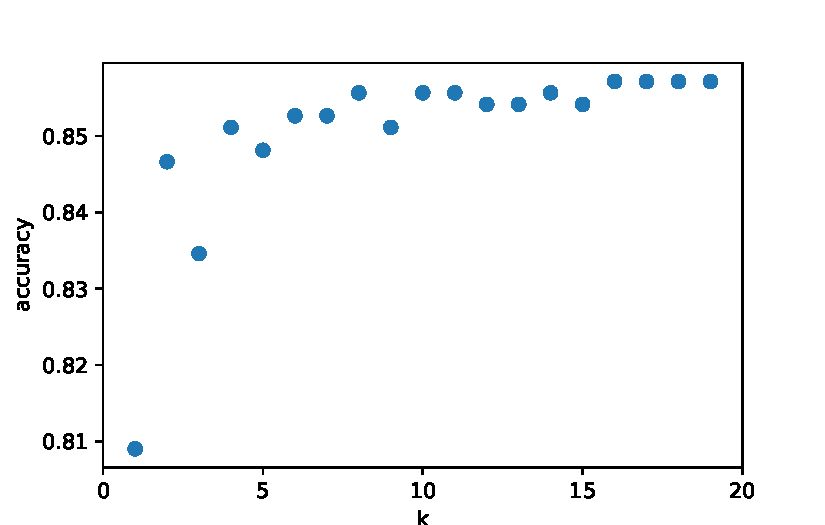
\includegraphics[keepaspectratio]{KnnNB_files/figure-pdf/mejor_modelo_python-1.pdf}}

\paragraph{Predicción de la variable
respuesta}\label{predicciuxf3n-de-la-variable-respuesta}

\subsection{R: R base}

La própia función que entrena el algoritmo ya devuelve las predicciones
del algoritmo de KNN.

\subsection{\texorpdfstring{R: Packages
\texttt{caret}}{R: Packages caret}}

\begin{Shaded}
\begin{Highlighting}[]
\FunctionTok{head}\NormalTok{(}\FunctionTok{predict}\NormalTok{(entrenamiento, }\AttributeTok{newdata =}\NormalTok{ X\_testC, }\AttributeTok{type =} \StringTok{"prob"}\NormalTok{), }\AttributeTok{n =} \DecValTok{10}\NormalTok{)}
\end{Highlighting}
\end{Shaded}

\begin{verbatim}
          No       Yes
1  0.8571429 0.1428571
2  0.8571429 0.1428571
3  1.0000000 0.0000000
4  0.7142857 0.2857143
5  0.8571429 0.1428571
6  0.8571429 0.1428571
7  1.0000000 0.0000000
8  1.0000000 0.0000000
9  0.7142857 0.2857143
10 0.8571429 0.1428571
\end{verbatim}

\subsection{Python}

\subparagraph{Predicción de la
etiqueta}\label{predicciuxf3n-de-la-etiqueta}

\begin{Shaded}
\begin{Highlighting}[]
\NormalTok{y\_predPy }\OperatorTok{=}\NormalTok{ knn.predict(X\_testPy)}
\NormalTok{y\_predPy[:}\DecValTok{20}\NormalTok{]}
\end{Highlighting}
\end{Shaded}

\begin{verbatim}
array(['No', 'No', 'No', 'No', 'No', 'No', 'No', 'No', 'No', 'No', 'No',
       'No', 'No', 'No', 'No', 'No', 'No', 'No', 'No', 'No'], dtype=object)
\end{verbatim}

\subparagraph{Predicción de pertenecer a cada
etiqueta}\label{predicciuxf3n-de-pertenecer-a-cada-etiqueta}

\begin{Shaded}
\begin{Highlighting}[]
\CommentTok{\# probability of getting output as 2 {-} benign cancer}
\NormalTok{knn.predict\_proba(X\_testPy)}
\end{Highlighting}
\end{Shaded}

\begin{verbatim}
array([[0.68421053, 0.31578947],
       [0.84210526, 0.15789474],
       [0.89473684, 0.10526316],
       ...,
       [0.89473684, 0.10526316],
       [1.        , 0.        ],
       [1.        , 0.        ]], shape=(665, 2))
\end{verbatim}

\paragraph{\texorpdfstring{Validación de la \emph{performance} del
modelo}{Validación de la performance del modelo}}\label{validaciuxf3n-de-la-performance-del-modelo}

\subsection{R: R base}

\begin{Shaded}
\begin{Highlighting}[]
\NormalTok{calc\_class\_err }\OtherTok{=} \ControlFlowTok{function}\NormalTok{(actual, predicted) \{}
  \FunctionTok{mean}\NormalTok{(actual }\SpecialCharTok{!=}\NormalTok{ predicted)}
\NormalTok{\}}
\end{Highlighting}
\end{Shaded}

\begin{Shaded}
\begin{Highlighting}[]
\FunctionTok{calc\_class\_err}\NormalTok{(}\AttributeTok{actual    =}\NormalTok{ y\_test,}
               \AttributeTok{predicted =} \FunctionTok{knn}\NormalTok{(}\AttributeTok{train =}\NormalTok{ X\_train,}
                               \AttributeTok{test  =}\NormalTok{ X\_test,}
                               \AttributeTok{cl    =}\NormalTok{ y\_train,}
                               \AttributeTok{k     =} \DecValTok{5}\NormalTok{))}
\end{Highlighting}
\end{Shaded}

\begin{verbatim}
[1] 0.1684211
\end{verbatim}

\begin{Shaded}
\begin{Highlighting}[]
\FunctionTok{max}\NormalTok{(}\FunctionTok{which}\NormalTok{(err\_k }\SpecialCharTok{==} \FunctionTok{min}\NormalTok{(err\_k)))}
\end{Highlighting}
\end{Shaded}

\begin{verbatim}
[1] 14
\end{verbatim}

\begin{Shaded}
\begin{Highlighting}[]
\NormalTok{predicciones }\OtherTok{\textless{}{-}} \FunctionTok{knn}\NormalTok{(}\AttributeTok{train =}\NormalTok{ X\_train, }\AttributeTok{test =}\NormalTok{ X\_test, }\AttributeTok{cl =}\NormalTok{ y\_train, }\AttributeTok{k =} \DecValTok{5}\NormalTok{)}
\FunctionTok{table}\NormalTok{(predicciones, y\_test)}
\end{Highlighting}
\end{Shaded}

\begin{verbatim}
            y_test
predicciones  No Yes
         No  539  90
         Yes  22  14
\end{verbatim}

\begin{Shaded}
\begin{Highlighting}[]
\CommentTok{\# Paquetes}
\FunctionTok{library}\NormalTok{(class)      }\CommentTok{\# knn}
\FunctionTok{library}\NormalTok{(ggplot2)    }\CommentTok{\# plotting}
\FunctionTok{library}\NormalTok{(dplyr)      }\CommentTok{\# \%\textgreater{}\%, mutate}
\FunctionTok{library}\NormalTok{(tidyr)}

\CommentTok{\# {-}{-}{-} Datos de entrada esperados {-}{-}{-}}
\CommentTok{\# X\_train, X\_test: data.frames/ matrices numéricas}
\CommentTok{\# y\_train, y\_test: vector/factor de etiquetas (clases)}

\NormalTok{k }\OtherTok{\textless{}{-}} \DecValTok{5}

\CommentTok{\# 1) PCA AJUSTADO EN TRAIN (con centrado y escalado). Proyectamos train y test.}
\NormalTok{pca }\OtherTok{\textless{}{-}} \FunctionTok{prcomp}\NormalTok{(X\_train, }\AttributeTok{center =} \ConstantTok{TRUE}\NormalTok{, }\AttributeTok{scale. =} \ConstantTok{TRUE}\NormalTok{)}

\NormalTok{Z\_train }\OtherTok{\textless{}{-}} \FunctionTok{predict}\NormalTok{(pca, }\AttributeTok{newdata =}\NormalTok{ X\_train)[, }\DecValTok{1}\SpecialCharTok{:}\DecValTok{2}\NormalTok{]}
\NormalTok{Z\_test  }\OtherTok{\textless{}{-}} \FunctionTok{predict}\NormalTok{(pca, }\AttributeTok{newdata =}\NormalTok{ X\_test)[, }\DecValTok{1}\SpecialCharTok{:}\DecValTok{2}\NormalTok{]}

\FunctionTok{colnames}\NormalTok{(Z\_train) }\OtherTok{\textless{}{-}} \FunctionTok{c}\NormalTok{(}\StringTok{"PC1"}\NormalTok{,}\StringTok{"PC2"}\NormalTok{)}
\FunctionTok{colnames}\NormalTok{(Z\_test)  }\OtherTok{\textless{}{-}} \FunctionTok{c}\NormalTok{(}\StringTok{"PC1"}\NormalTok{,}\StringTok{"PC2"}\NormalTok{)}

\CommentTok{\# 2) Rango para el grid (usamos TRAIN para coherencia)}
\NormalTok{h }\OtherTok{\textless{}{-}} \FloatTok{0.02}
\NormalTok{x\_min }\OtherTok{\textless{}{-}} \FunctionTok{min}\NormalTok{(Z\_train[,}\DecValTok{1}\NormalTok{]) }\SpecialCharTok{{-}} \DecValTok{1}\NormalTok{; x\_max }\OtherTok{\textless{}{-}} \FunctionTok{max}\NormalTok{(Z\_train[,}\DecValTok{1}\NormalTok{]) }\SpecialCharTok{+} \DecValTok{1}
\NormalTok{y\_min }\OtherTok{\textless{}{-}} \FunctionTok{min}\NormalTok{(Z\_train[,}\DecValTok{2}\NormalTok{]) }\SpecialCharTok{{-}} \DecValTok{1}\NormalTok{; y\_max }\OtherTok{\textless{}{-}} \FunctionTok{max}\NormalTok{(Z\_train[,}\DecValTok{2}\NormalTok{]) }\SpecialCharTok{+} \DecValTok{1}

\NormalTok{grid }\OtherTok{\textless{}{-}} \FunctionTok{expand.grid}\NormalTok{(}
  \AttributeTok{PC1 =} \FunctionTok{seq}\NormalTok{(x\_min, x\_max, }\AttributeTok{by =}\NormalTok{ h),}
  \AttributeTok{PC2 =} \FunctionTok{seq}\NormalTok{(y\_min, y\_max, }\AttributeTok{by =}\NormalTok{ h)}
\NormalTok{)}

\CommentTok{\# 3) kNN en el plano PCA (class::knn no "entrena"; predice dado train/test)}
\CommentTok{\#    Usamos las coordenadas PCA de train como "train", y el grid como "test".}
\CommentTok{\#    Asegura que y\_train sea factor.}
\NormalTok{y\_train }\OtherTok{\textless{}{-}} \FunctionTok{factor}\NormalTok{(y\_train)}
\NormalTok{y\_test  }\OtherTok{\textless{}{-}} \FunctionTok{factor}\NormalTok{(y\_test, }\AttributeTok{levels =} \FunctionTok{levels}\NormalTok{(y\_train))}

\NormalTok{grid\_pred }\OtherTok{\textless{}{-}} \FunctionTok{knn}\NormalTok{(}
  \AttributeTok{train =}\NormalTok{ Z\_train,}
  \AttributeTok{test  =}\NormalTok{ grid,}
  \AttributeTok{cl    =}\NormalTok{ y\_train,}
  \AttributeTok{k     =}\NormalTok{ k}
\NormalTok{)}

\NormalTok{grid}\SpecialCharTok{$}\NormalTok{pred }\OtherTok{\textless{}{-}} \FunctionTok{factor}\NormalTok{(grid\_pred, }\AttributeTok{levels =} \FunctionTok{levels}\NormalTok{(y\_train))}

\CommentTok{\# 4) Data frames para puntos}
\NormalTok{df\_train }\OtherTok{\textless{}{-}} \FunctionTok{data.frame}\NormalTok{(Z\_train, }\AttributeTok{clase =}\NormalTok{ y\_train, }\AttributeTok{split =} \StringTok{"Train"}\NormalTok{)}
\NormalTok{df\_test  }\OtherTok{\textless{}{-}} \FunctionTok{data.frame}\NormalTok{(Z\_test,  }\AttributeTok{clase =}\NormalTok{ y\_test,  }\AttributeTok{split =} \StringTok{"Test"}\NormalTok{)}

\CommentTok{\# 5) Paleta (ajusta si hay \textgreater{}2 clases)}
\NormalTok{pal\_cls  }\OtherTok{\textless{}{-}} \FunctionTok{c}\NormalTok{(}\StringTok{"\#FF0000"}\NormalTok{, }\StringTok{"\#00ffff"}\NormalTok{)           }\CommentTok{\# puntos (clases)}
\NormalTok{pal\_fill }\OtherTok{\textless{}{-}} \FunctionTok{c}\NormalTok{(}\StringTok{"\#FFAAAA"}\NormalTok{, }\StringTok{"\#b3ffff"}\NormalTok{)           }\CommentTok{\# fondo (clases)}
\FunctionTok{names}\NormalTok{(pal\_cls)  }\OtherTok{\textless{}{-}} \FunctionTok{levels}\NormalTok{(y\_train)}
\FunctionTok{names}\NormalTok{(pal\_fill) }\OtherTok{\textless{}{-}} \FunctionTok{levels}\NormalTok{(y\_train)}

\CommentTok{\# 6) Plot: fondo (grid) + puntos (train/test)}
\FunctionTok{ggplot}\NormalTok{() }\SpecialCharTok{+}
  \FunctionTok{geom\_raster}\NormalTok{(}\AttributeTok{data =}\NormalTok{ grid, }\FunctionTok{aes}\NormalTok{(}\AttributeTok{x =}\NormalTok{ PC1, }\AttributeTok{y =}\NormalTok{ PC2, }\AttributeTok{fill =}\NormalTok{ pred), }\AttributeTok{alpha =} \DecValTok{1}\NormalTok{) }\SpecialCharTok{+}
  \FunctionTok{scale\_fill\_manual}\NormalTok{(}\AttributeTok{values =}\NormalTok{ pal\_fill, }\AttributeTok{name =} \StringTok{"Clase (fondo)"}\NormalTok{) }\SpecialCharTok{+}
  \FunctionTok{geom\_point}\NormalTok{(}\AttributeTok{data =}\NormalTok{ df\_train, }\FunctionTok{aes}\NormalTok{(PC1, PC2, }\AttributeTok{color =}\NormalTok{ clase), }\AttributeTok{size =} \FloatTok{1.8}\NormalTok{, }\AttributeTok{stroke =}\NormalTok{ .}\DecValTok{2}\NormalTok{) }\SpecialCharTok{+}
  \FunctionTok{geom\_point}\NormalTok{(}\AttributeTok{data =}\NormalTok{ df\_test,  }\FunctionTok{aes}\NormalTok{(PC1, PC2, }\AttributeTok{color =}\NormalTok{ clase), }\AttributeTok{size =} \FloatTok{2.2}\NormalTok{, }\AttributeTok{stroke =}\NormalTok{ .}\DecValTok{2}\NormalTok{, }\AttributeTok{shape =} \DecValTok{21}\NormalTok{) }\SpecialCharTok{+}
  \FunctionTok{scale\_color\_manual}\NormalTok{(}\AttributeTok{values =}\NormalTok{ pal\_cls, }\AttributeTok{name =} \StringTok{"Clase (puntos)"}\NormalTok{) }\SpecialCharTok{+}
  \FunctionTok{labs}\NormalTok{(}
    \AttributeTok{title =} \FunctionTok{sprintf}\NormalTok{(}\StringTok{"Frontera kNN en plano PCA (k=\%d, weights=\textquotesingle{}distance\textquotesingle{})"}\NormalTok{, k),}
    \AttributeTok{x =} \StringTok{"PC1"}\NormalTok{, }\AttributeTok{y =} \StringTok{"PC2"}
\NormalTok{  ) }\SpecialCharTok{+}
  \FunctionTok{coord\_equal}\NormalTok{(}\AttributeTok{expand =} \ConstantTok{FALSE}\NormalTok{, }\AttributeTok{xlim =} \FunctionTok{c}\NormalTok{(x\_min, x\_max), }\AttributeTok{ylim =} \FunctionTok{c}\NormalTok{(y\_min, y\_max)) }\SpecialCharTok{+}
  \FunctionTok{theme\_minimal}\NormalTok{() }\SpecialCharTok{+}
  \FunctionTok{theme}\NormalTok{(}\AttributeTok{legend.position =} \StringTok{"right"}\NormalTok{)}
\end{Highlighting}
\end{Shaded}

\pandocbounded{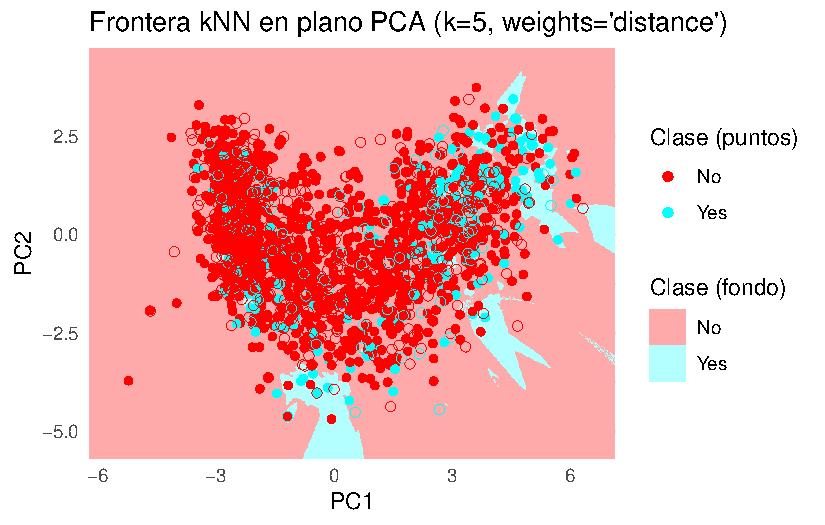
\includegraphics[keepaspectratio]{KnnNB_files/figure-pdf/grafico_pca_modelo-1.pdf}}

\subsection{\texorpdfstring{R: Packages
\texttt{caret}}{R: Packages caret}}

\begin{Shaded}
\begin{Highlighting}[]
\NormalTok{caret}\SpecialCharTok{::}\FunctionTok{confusionMatrix}\NormalTok{(}\FunctionTok{predict}\NormalTok{(entrenamiento, }\AttributeTok{newdata =}\NormalTok{ X\_testC), y\_testC)}
\end{Highlighting}
\end{Shaded}

\begin{verbatim}
Confusion Matrix and Statistics

          Reference
Prediction  No Yes
       No  555  89
       Yes   9  10
                                          
               Accuracy : 0.8522          
                 95% CI : (0.8229, 0.8783)
    No Information Rate : 0.8507          
    P-Value [Acc > NIR] : 0.4833          
                                          
                  Kappa : 0.1275          
                                          
 Mcnemar's Test P-Value : 1.461e-15       
                                          
            Sensitivity : 0.9840          
            Specificity : 0.1010          
         Pos Pred Value : 0.8618          
         Neg Pred Value : 0.5263          
             Prevalence : 0.8507          
         Detection Rate : 0.8371          
   Detection Prevalence : 0.9713          
      Balanced Accuracy : 0.5425          
                                          
       'Positive' Class : No              
                                          
\end{verbatim}

\begin{Shaded}
\begin{Highlighting}[]
\FunctionTok{library}\NormalTok{(ggplot2)}
\FunctionTok{library}\NormalTok{(reshape2)}

\CommentTok{\# Crear matriz de confusión como tabla}
\NormalTok{conf\_tbl }\OtherTok{\textless{}{-}} \FunctionTok{table}\NormalTok{(}\AttributeTok{Predicted =} \FunctionTok{predict}\NormalTok{(entrenamiento, }\AttributeTok{newdata =}\NormalTok{ X\_testC), }\AttributeTok{Actual =}\NormalTok{ y\_testC)}

\CommentTok{\# Convertir a data.frame para ggplot}
\NormalTok{conf\_df }\OtherTok{\textless{}{-}} \FunctionTok{as.data.frame}\NormalTok{(conf\_tbl)}
\FunctionTok{colnames}\NormalTok{(conf\_df) }\OtherTok{\textless{}{-}} \FunctionTok{c}\NormalTok{(}\StringTok{"Predicted"}\NormalTok{, }\StringTok{"Actual"}\NormalTok{, }\StringTok{"Freq"}\NormalTok{)}

\CommentTok{\# Visualización con ggplot2}
\FunctionTok{ggplot}\NormalTok{(conf\_df, }\FunctionTok{aes}\NormalTok{(}\AttributeTok{x =}\NormalTok{ Actual, }\AttributeTok{y =}\NormalTok{ Predicted, }\AttributeTok{fill =}\NormalTok{ Freq)) }\SpecialCharTok{+}
  \FunctionTok{geom\_tile}\NormalTok{(}\AttributeTok{color =} \StringTok{"white"}\NormalTok{) }\SpecialCharTok{+}
  \FunctionTok{geom\_text}\NormalTok{(}\FunctionTok{aes}\NormalTok{(}\AttributeTok{label =}\NormalTok{ Freq), }\AttributeTok{size =} \DecValTok{5}\NormalTok{) }\SpecialCharTok{+}
  \FunctionTok{scale\_fill\_gradient}\NormalTok{(}\AttributeTok{low =} \StringTok{"\#f7fcf0"}\NormalTok{, }\AttributeTok{high =} \StringTok{"\#084081"}\NormalTok{) }\SpecialCharTok{+}
  \FunctionTok{labs}\NormalTok{(}\AttributeTok{title =} \StringTok{"Matriz de confusión"}\NormalTok{, }\AttributeTok{x =} \StringTok{"Valor real"}\NormalTok{, }\AttributeTok{y =} \StringTok{"Predicción"}\NormalTok{) }\SpecialCharTok{+}
  \FunctionTok{theme\_minimal}\NormalTok{()}
\end{Highlighting}
\end{Shaded}

\pandocbounded{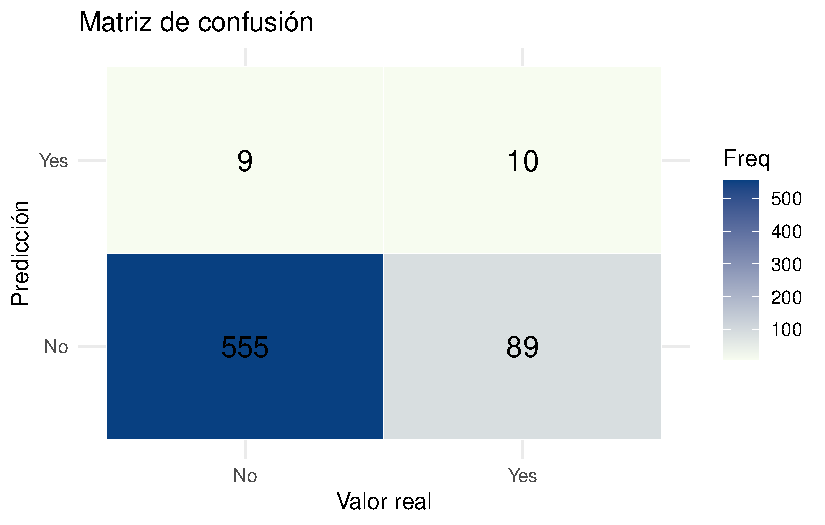
\includegraphics[keepaspectratio]{KnnNB_files/figure-pdf/confusion_matrix_ggplot2-1.pdf}}

\begin{Shaded}
\begin{Highlighting}[]
\FunctionTok{library}\NormalTok{(caret)}
\FunctionTok{library}\NormalTok{(ggplot2)}
\FunctionTok{library}\NormalTok{(dplyr)}

\CommentTok{\# {-}{-}{-} Si X\_trainC incluye la columna \textquotesingle{}Response\textquotesingle{}, separamos:}
\CommentTok{\#     (si ya la tienes separada, omite estas dos líneas y usa tus objetos)}
\NormalTok{y\_trainC }\OtherTok{\textless{}{-}} \FunctionTok{factor}\NormalTok{(X\_trainC}\SpecialCharTok{$}\NormalTok{Response)}
\NormalTok{X\_train\_num }\OtherTok{\textless{}{-}}\NormalTok{ X\_trainC[, }\FunctionTok{setdiff}\NormalTok{(}\FunctionTok{names}\NormalTok{(X\_trainC), }\StringTok{"Response"}\NormalTok{), drop }\OtherTok{=} \ConstantTok{FALSE}\NormalTok{]}

\CommentTok{\# Asegura que los predictores son numéricos}
\NormalTok{X\_train\_num[] }\OtherTok{\textless{}{-}} \FunctionTok{lapply}\NormalTok{(X\_train\_num, }\ControlFlowTok{function}\NormalTok{(col) }\FunctionTok{as.numeric}\NormalTok{(}\FunctionTok{as.character}\NormalTok{(col)))}

\CommentTok{\# 1) Preprocesado SOLO sobre predictores (center, scale, pca=2)}
\NormalTok{preproc }\OtherTok{\textless{}{-}} \FunctionTok{preProcess}\NormalTok{(X\_train\_num, }\AttributeTok{method =} \FunctionTok{c}\NormalTok{(}\StringTok{"center"}\NormalTok{, }\StringTok{"scale"}\NormalTok{, }\StringTok{"pca"}\NormalTok{), }\AttributeTok{pcaComp =} \DecValTok{2}\NormalTok{)}

\NormalTok{Z\_train }\OtherTok{\textless{}{-}} \FunctionTok{predict}\NormalTok{(preproc, X\_train\_num)  }\CommentTok{\# tendrá columnas PC1 y PC2}

\CommentTok{\# {-}{-}{-} Prepara también el test de forma consistente {-}{-}{-}}
\CommentTok{\# Si X\_testC tiene \textquotesingle{}Response\textquotesingle{}, sepárala:}
\ControlFlowTok{if}\NormalTok{ (}\StringTok{"Response"} \SpecialCharTok{\%in\%} \FunctionTok{names}\NormalTok{(X\_testC)) \{}
\NormalTok{  y\_testC  }\OtherTok{\textless{}{-}} \FunctionTok{factor}\NormalTok{(X\_testC}\SpecialCharTok{$}\NormalTok{Response, }\AttributeTok{levels =} \FunctionTok{levels}\NormalTok{(y\_trainC))}
\NormalTok{  X\_test\_num }\OtherTok{\textless{}{-}}\NormalTok{ X\_testC[, }\FunctionTok{setdiff}\NormalTok{(}\FunctionTok{names}\NormalTok{(X\_testC), }\StringTok{"Response"}\NormalTok{), drop }\OtherTok{=} \ConstantTok{FALSE}\NormalTok{]}
\NormalTok{\} }\ControlFlowTok{else}\NormalTok{ \{}
  \CommentTok{\# si ya tienes y\_testC aparte:}
\NormalTok{  X\_test\_num }\OtherTok{\textless{}{-}}\NormalTok{ X\_testC}
\NormalTok{  y\_testC    }\OtherTok{\textless{}{-}} \FunctionTok{factor}\NormalTok{(y\_testC, }\AttributeTok{levels =} \FunctionTok{levels}\NormalTok{(y\_trainC))}
\NormalTok{\}}
\NormalTok{X\_test\_num[] }\OtherTok{\textless{}{-}} \FunctionTok{lapply}\NormalTok{(X\_test\_num, }\ControlFlowTok{function}\NormalTok{(col) }\FunctionTok{as.numeric}\NormalTok{(}\FunctionTok{as.character}\NormalTok{(col)))}
\NormalTok{Z\_test }\OtherTok{\textless{}{-}} \FunctionTok{predict}\NormalTok{(preproc, X\_test\_num)}

\CommentTok{\# 2) Control de entrenamiento (CV estratificada)}
\NormalTok{ctrl }\OtherTok{\textless{}{-}} \FunctionTok{trainControl}\NormalTok{(}\AttributeTok{method =} \StringTok{"cv"}\NormalTok{, }\AttributeTok{number =} \DecValTok{5}\NormalTok{)}

\CommentTok{\# 3) Entrenar kNN en el espacio PCA}
\NormalTok{k }\OtherTok{\textless{}{-}} \DecValTok{5}
\NormalTok{modelo\_knn }\OtherTok{\textless{}{-}} \FunctionTok{train}\NormalTok{(}
  \AttributeTok{x =}\NormalTok{ Z\_train,}
  \AttributeTok{y =}\NormalTok{ y\_trainC,}
  \AttributeTok{method =} \StringTok{"knn"}\NormalTok{,}
  \AttributeTok{tuneGrid =} \FunctionTok{data.frame}\NormalTok{(}\AttributeTok{k =}\NormalTok{ k),}
  \AttributeTok{trControl =}\NormalTok{ ctrl,}
  \AttributeTok{metric =} \StringTok{"Accuracy"}
\NormalTok{)}

\CommentTok{\# 3) Grid en el plano PCA (rango del TRAIN)}
\NormalTok{h }\OtherTok{\textless{}{-}} \FloatTok{0.02}
\NormalTok{x\_min }\OtherTok{\textless{}{-}} \FunctionTok{min}\NormalTok{(Z\_train}\SpecialCharTok{$}\NormalTok{PC1) }\SpecialCharTok{{-}} \DecValTok{1}\NormalTok{; x\_max }\OtherTok{\textless{}{-}} \FunctionTok{max}\NormalTok{(Z\_train}\SpecialCharTok{$}\NormalTok{PC1) }\SpecialCharTok{+} \DecValTok{1}
\NormalTok{y\_min }\OtherTok{\textless{}{-}} \FunctionTok{min}\NormalTok{(Z\_train}\SpecialCharTok{$}\NormalTok{PC2) }\SpecialCharTok{{-}} \DecValTok{1}\NormalTok{; y\_max }\OtherTok{\textless{}{-}} \FunctionTok{max}\NormalTok{(Z\_train}\SpecialCharTok{$}\NormalTok{PC2) }\SpecialCharTok{+} \DecValTok{1}

\NormalTok{grid }\OtherTok{\textless{}{-}} \FunctionTok{expand.grid}\NormalTok{(}
  \AttributeTok{PC1 =} \FunctionTok{seq}\NormalTok{(x\_min, x\_max, }\AttributeTok{by =}\NormalTok{ h),}
  \AttributeTok{PC2 =} \FunctionTok{seq}\NormalTok{(y\_min, y\_max, }\AttributeTok{by =}\NormalTok{ h)}
\NormalTok{)}

\CommentTok{\# 4) Predicción del fondo en el grid}
\NormalTok{grid}\SpecialCharTok{$}\NormalTok{pred }\OtherTok{\textless{}{-}} \FunctionTok{predict}\NormalTok{(modelo\_knn, }\AttributeTok{newdata =}\NormalTok{ grid)}

\CommentTok{\# 5) Data frames para puntos}
\NormalTok{df\_train }\OtherTok{\textless{}{-}} \FunctionTok{data.frame}\NormalTok{(Z\_train, }\AttributeTok{clase =}\NormalTok{ y\_trainC, }\AttributeTok{split =} \StringTok{"Train"}\NormalTok{)}
\NormalTok{df\_test  }\OtherTok{\textless{}{-}} \FunctionTok{data.frame}\NormalTok{(Z\_test,  }\AttributeTok{clase =}\NormalTok{ y\_testC,  }\AttributeTok{split =} \StringTok{"Test"}\NormalTok{)}

\CommentTok{\# 6) Paletas}
\NormalTok{pal\_cls  }\OtherTok{\textless{}{-}} \FunctionTok{c}\NormalTok{(}\StringTok{"\#FF0000"}\NormalTok{, }\StringTok{"\#00ffff"}\NormalTok{)}
\NormalTok{pal\_fill }\OtherTok{\textless{}{-}} \FunctionTok{c}\NormalTok{(}\StringTok{"\#FFAAAA"}\NormalTok{, }\StringTok{"\#b3ffff"}\NormalTok{)}
\FunctionTok{names}\NormalTok{(pal\_cls)  }\OtherTok{\textless{}{-}} \FunctionTok{levels}\NormalTok{(y\_trainC)}
\FunctionTok{names}\NormalTok{(pal\_fill) }\OtherTok{\textless{}{-}} \FunctionTok{levels}\NormalTok{(y\_trainC)}

\CommentTok{\# 7) Plot}
\FunctionTok{ggplot}\NormalTok{() }\SpecialCharTok{+}
  \FunctionTok{geom\_raster}\NormalTok{(}\AttributeTok{data =}\NormalTok{ grid, }\FunctionTok{aes}\NormalTok{(}\AttributeTok{x =}\NormalTok{ PC1, }\AttributeTok{y =}\NormalTok{ PC2, }\AttributeTok{fill =}\NormalTok{ pred), }\AttributeTok{alpha =} \DecValTok{1}\NormalTok{) }\SpecialCharTok{+}
  \FunctionTok{scale\_fill\_manual}\NormalTok{(}\AttributeTok{values =}\NormalTok{ pal\_fill, }\AttributeTok{name =} \StringTok{"Clase (fondo)"}\NormalTok{) }\SpecialCharTok{+}
  \FunctionTok{geom\_point}\NormalTok{(}\AttributeTok{data =}\NormalTok{ df\_train, }\FunctionTok{aes}\NormalTok{(PC1, PC2, }\AttributeTok{color =}\NormalTok{ clase), }\AttributeTok{size =} \FloatTok{1.8}\NormalTok{, }\AttributeTok{stroke =}\NormalTok{ .}\DecValTok{2}\NormalTok{) }\SpecialCharTok{+}
  \FunctionTok{geom\_point}\NormalTok{(}\AttributeTok{data =}\NormalTok{ df\_test,  }\FunctionTok{aes}\NormalTok{(PC1, PC2, }\AttributeTok{color =}\NormalTok{ clase), }\AttributeTok{size =} \FloatTok{2.2}\NormalTok{, }\AttributeTok{stroke =}\NormalTok{ .}\DecValTok{2}\NormalTok{, }\AttributeTok{shape =} \DecValTok{21}\NormalTok{) }\SpecialCharTok{+}
  \FunctionTok{scale\_color\_manual}\NormalTok{(}\AttributeTok{values =}\NormalTok{ pal\_cls, }\AttributeTok{name =} \StringTok{"Clase (puntos)"}\NormalTok{) }\SpecialCharTok{+}
  \FunctionTok{labs}\NormalTok{(}
    \AttributeTok{title =} \FunctionTok{sprintf}\NormalTok{(}\StringTok{"Frontera kNN en plano PCA (k=\%d)"}\NormalTok{, k),}
    \AttributeTok{x =} \StringTok{"PC1"}\NormalTok{, }\AttributeTok{y =} \StringTok{"PC2"}
\NormalTok{  ) }\SpecialCharTok{+}
  \FunctionTok{coord\_equal}\NormalTok{(}\AttributeTok{expand =} \ConstantTok{FALSE}\NormalTok{, }\AttributeTok{xlim =} \FunctionTok{c}\NormalTok{(x\_min, x\_max), }\AttributeTok{ylim =} \FunctionTok{c}\NormalTok{(y\_min, y\_max)) }\SpecialCharTok{+}
  \FunctionTok{theme\_minimal}\NormalTok{() }\SpecialCharTok{+}
  \FunctionTok{theme}\NormalTok{(}\AttributeTok{legend.position =} \StringTok{"right"}\NormalTok{)}
\end{Highlighting}
\end{Shaded}

\pandocbounded{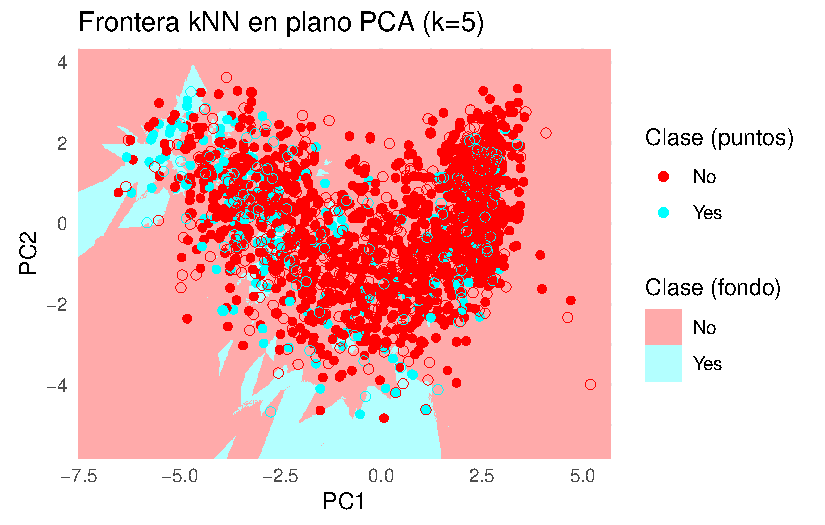
\includegraphics[keepaspectratio]{KnnNB_files/figure-pdf/grafico_pca_caret-1.pdf}}

\subsection{Python}

\begin{Shaded}
\begin{Highlighting}[]
\ImportTok{from}\NormalTok{ sklearn.metrics }\ImportTok{import}\NormalTok{ accuracy\_score}
\BuiltInTok{print}\NormalTok{(}\StringTok{\textquotesingle{}Model accuracy score: }\SpecialCharTok{\{0:0.4f\}}\StringTok{\textquotesingle{}}\NormalTok{. }\BuiltInTok{format}\NormalTok{(accuracy\_score(y\_testPy, y\_predPy)))}
\end{Highlighting}
\end{Shaded}

\begin{verbatim}
Model accuracy score: 0.8571
\end{verbatim}

\paragraph{Estudio del sobreajuste}\label{estudio-del-sobreajuste}

\begin{Shaded}
\begin{Highlighting}[]
\BuiltInTok{print}\NormalTok{(}\StringTok{\textquotesingle{}Training set score: }\SpecialCharTok{\{:.4f\}}\StringTok{\textquotesingle{}}\NormalTok{.}\BuiltInTok{format}\NormalTok{(knn.score(X\_trainPy, y\_trainPy)))}
\end{Highlighting}
\end{Shaded}

\begin{verbatim}
Training set score: 0.8478
\end{verbatim}

\begin{Shaded}
\begin{Highlighting}[]
\BuiltInTok{print}\NormalTok{(}\StringTok{\textquotesingle{}Test set score: }\SpecialCharTok{\{:.4f\}}\StringTok{\textquotesingle{}}\NormalTok{.}\BuiltInTok{format}\NormalTok{(knn.score(X\_testPy, y\_testPy)))}
\end{Highlighting}
\end{Shaded}

\begin{verbatim}
Test set score: 0.8571
\end{verbatim}

\begin{Shaded}
\begin{Highlighting}[]
\ImportTok{import}\NormalTok{ seaborn }\ImportTok{as}\NormalTok{ sns }\CommentTok{\# for data visualization}
\ImportTok{from}\NormalTok{ sklearn.metrics }\ImportTok{import}\NormalTok{ confusion\_matrix}

\CommentTok{\# visualize confusion matrix with seaborn heatmap}

\NormalTok{plt.figure(figsize}\OperatorTok{=}\NormalTok{(}\DecValTok{6}\NormalTok{,}\DecValTok{4}\NormalTok{))}
\NormalTok{confMatrix }\OperatorTok{=}\NormalTok{ confusion\_matrix(y\_testPy, y\_predPy)}
\NormalTok{cm\_matrix }\OperatorTok{=}\NormalTok{ pd.DataFrame(data}\OperatorTok{=}\NormalTok{confMatrix, columns}\OperatorTok{=}\NormalTok{[}\StringTok{\textquotesingle{}Actual Positive:1\textquotesingle{}}\NormalTok{, }\StringTok{\textquotesingle{}Actual Negative:0\textquotesingle{}}\NormalTok{], index}\OperatorTok{=}\NormalTok{[}\StringTok{\textquotesingle{}Predict Positive:1\textquotesingle{}}\NormalTok{, }\StringTok{\textquotesingle{}Predict Negative:0\textquotesingle{}}\NormalTok{])}

\NormalTok{sns.heatmap(cm\_matrix, annot}\OperatorTok{=}\VariableTok{True}\NormalTok{, fmt}\OperatorTok{=}\StringTok{\textquotesingle{}d\textquotesingle{}}\NormalTok{, cmap}\OperatorTok{=}\StringTok{\textquotesingle{}YlGnBu\textquotesingle{}}\NormalTok{)}
\end{Highlighting}
\end{Shaded}

\pandocbounded{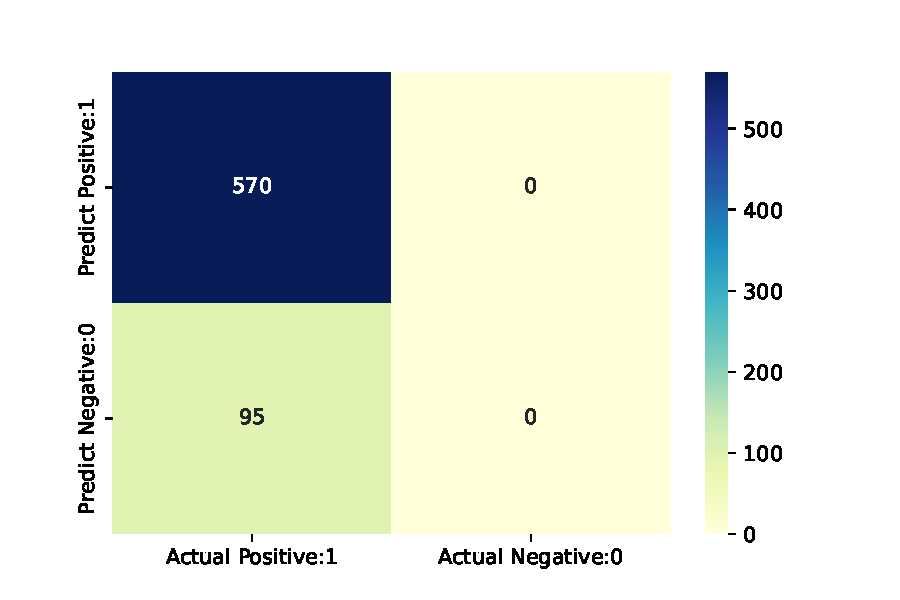
\includegraphics[keepaspectratio]{KnnNB_files/figure-pdf/heatmap_matriz_confusion_python-1.pdf}}

\begin{Shaded}
\begin{Highlighting}[]
\ImportTok{from}\NormalTok{ sklearn.metrics }\ImportTok{import}\NormalTok{ classification\_report}
\BuiltInTok{print}\NormalTok{(classification\_report(y\_testPy, y\_predPy))}
\end{Highlighting}
\end{Shaded}

\begin{verbatim}
              precision    recall  f1-score   support

          No       0.86      1.00      0.92       570
         Yes       0.00      0.00      0.00        95

    accuracy                           0.86       665
   macro avg       0.43      0.50      0.46       665
weighted avg       0.73      0.86      0.79       665
\end{verbatim}

\begin{Shaded}
\begin{Highlighting}[]
\ImportTok{import}\NormalTok{ numpy }\ImportTok{as}\NormalTok{ np}
\ImportTok{import}\NormalTok{ matplotlib.pyplot }\ImportTok{as}\NormalTok{ plt}
\ImportTok{from}\NormalTok{ matplotlib.colors }\ImportTok{import}\NormalTok{ ListedColormap}
\ImportTok{import}\NormalTok{ matplotlib.patches }\ImportTok{as}\NormalTok{ mpatches}

\ImportTok{from}\NormalTok{ sklearn.preprocessing }\ImportTok{import}\NormalTok{ StandardScaler, LabelEncoder}
\ImportTok{from}\NormalTok{ sklearn.decomposition }\ImportTok{import}\NormalTok{ PCA}
\ImportTok{from}\NormalTok{ sklearn.neighbors }\ImportTok{import}\NormalTok{ KNeighborsClassifier}

\CommentTok{\# ==== Parámetros ====}
\NormalTok{n\_neighbors }\OperatorTok{=} \DecValTok{5}
\NormalTok{weights }\OperatorTok{=} \StringTok{\textquotesingle{}distance\textquotesingle{}}
\NormalTok{h }\OperatorTok{=} \FloatTok{0.02}

\CommentTok{\# ==== 0) Asegurar tipos correctos ====}
\NormalTok{X\_trainPy }\OperatorTok{=}\NormalTok{ np.asarray(X\_trainPy, dtype}\OperatorTok{=}\BuiltInTok{float}\NormalTok{)}
\NormalTok{X\_testPy  }\OperatorTok{=}\NormalTok{ np.asarray(X\_testPy,  dtype}\OperatorTok{=}\BuiltInTok{float}\NormalTok{)}
\NormalTok{y\_trainPy }\OperatorTok{=}\NormalTok{ np.asarray(y\_trainPy)}
\NormalTok{y\_testPy  }\OperatorTok{=}\NormalTok{ np.asarray(y\_testPy)}

\CommentTok{\# Codificar etiquetas a enteros (necesario para c= y pcolormesh)}
\NormalTok{le }\OperatorTok{=}\NormalTok{ LabelEncoder()}
\NormalTok{y\_train\_num }\OperatorTok{=}\NormalTok{ le.fit\_transform(y\_trainPy)}
\NormalTok{y\_test\_num  }\OperatorTok{=}\NormalTok{ le.transform(y\_testPy)}

\CommentTok{\# ==== 1) Estandarizar con medias/SD de train + PCA en train ====}
\NormalTok{scaler }\OperatorTok{=}\NormalTok{ StandardScaler()}
\NormalTok{X\_train\_scaled }\OperatorTok{=}\NormalTok{ scaler.fit\_transform(X\_trainPy)}
\NormalTok{X\_test\_scaled  }\OperatorTok{=}\NormalTok{ scaler.transform(X\_testPy)}

\NormalTok{pca }\OperatorTok{=}\NormalTok{ PCA(n\_components}\OperatorTok{=}\DecValTok{2}\NormalTok{, random\_state}\OperatorTok{=}\DecValTok{0}\NormalTok{)}
\NormalTok{Z\_train }\OperatorTok{=}\NormalTok{ pca.fit\_transform(X\_train\_scaled).astype(}\BuiltInTok{float}\NormalTok{)   }\CommentTok{\# coords PCA train}
\NormalTok{Z\_test  }\OperatorTok{=}\NormalTok{ pca.transform(X\_test\_scaled).astype(}\BuiltInTok{float}\NormalTok{)        }\CommentTok{\# coords PCA test}

\CommentTok{\# ==== 2) Entrenar KNN en el espacio PCA (train) ====}
\NormalTok{clf }\OperatorTok{=}\NormalTok{ KNeighborsClassifier(n\_neighbors}\OperatorTok{=}\NormalTok{n\_neighbors, weights}\OperatorTok{=}\NormalTok{weights)}
\NormalTok{clf.fit(Z\_train, y\_train\_num)}
\end{Highlighting}
\end{Shaded}

\begin{verbatim}
KNeighborsClassifier(weights='distance')
\end{verbatim}

\begin{Shaded}
\begin{Highlighting}[]
\CommentTok{\# ==== 3) Mallado en el plano PCA (usando rango de TRAIN para coherencia) ====}
\NormalTok{x\_min, x\_max }\OperatorTok{=}\NormalTok{ Z\_train[:, }\DecValTok{0}\NormalTok{].}\BuiltInTok{min}\NormalTok{() }\OperatorTok{{-}} \DecValTok{1}\NormalTok{, Z\_train[:, }\DecValTok{0}\NormalTok{].}\BuiltInTok{max}\NormalTok{() }\OperatorTok{+} \DecValTok{1}
\NormalTok{y\_min, y\_max }\OperatorTok{=}\NormalTok{ Z\_train[:, }\DecValTok{1}\NormalTok{].}\BuiltInTok{min}\NormalTok{() }\OperatorTok{{-}} \DecValTok{1}\NormalTok{, Z\_train[:, }\DecValTok{1}\NormalTok{].}\BuiltInTok{max}\NormalTok{() }\OperatorTok{+} \DecValTok{1}

\NormalTok{xx, yy }\OperatorTok{=}\NormalTok{ np.meshgrid(np.arange(x\_min, x\_max, h),}
\NormalTok{                     np.arange(y\_min, y\_max, h))}

\NormalTok{Z\_grid\_pred\_num }\OperatorTok{=}\NormalTok{ clf.predict(np.c\_[xx.ravel(), yy.ravel()]).reshape(xx.shape)}

\CommentTok{\# ==== 4) Paletas (binario por tus colores; amplía si hay \textgreater{}2 clases) ====}
\NormalTok{cmap\_light }\OperatorTok{=}\NormalTok{ ListedColormap([}\StringTok{\textquotesingle{}\#FFAAAA\textquotesingle{}}\NormalTok{, }\StringTok{\textquotesingle{}\#b3ffff\textquotesingle{}}\NormalTok{])}
\NormalTok{cmap\_bold  }\OperatorTok{=}\NormalTok{ ListedColormap([}\StringTok{\textquotesingle{}\#FF0000\textquotesingle{}}\NormalTok{, }\StringTok{\textquotesingle{}\#00ffff\textquotesingle{}}\NormalTok{])}

\CommentTok{\# ==== 5) Plot fondo + puntos ====}
\NormalTok{plt.figure(figsize}\OperatorTok{=}\NormalTok{(}\DecValTok{7}\NormalTok{, }\DecValTok{5}\NormalTok{))}
\NormalTok{plt.pcolormesh(xx, yy, Z\_grid\_pred\_num, cmap}\OperatorTok{=}\NormalTok{cmap\_light, shading}\OperatorTok{=}\StringTok{\textquotesingle{}auto\textquotesingle{}}\NormalTok{)}

\CommentTok{\# Train}
\NormalTok{plt.scatter(Z\_train[:, }\DecValTok{0}\NormalTok{], Z\_train[:, }\DecValTok{1}\NormalTok{], c}\OperatorTok{=}\NormalTok{y\_train\_num, cmap}\OperatorTok{=}\NormalTok{cmap\_bold,}
\NormalTok{            edgecolor}\OperatorTok{=}\StringTok{\textquotesingle{}k\textquotesingle{}}\NormalTok{, s}\OperatorTok{=}\DecValTok{25}\NormalTok{, alpha}\OperatorTok{=}\FloatTok{0.8}\NormalTok{, label}\OperatorTok{=}\StringTok{\textquotesingle{}Train\textquotesingle{}}\NormalTok{)}

\CommentTok{\# Test}
\NormalTok{plt.scatter(Z\_test[:, }\DecValTok{0}\NormalTok{],  Z\_test[:, }\DecValTok{1}\NormalTok{],  c}\OperatorTok{=}\NormalTok{y\_test\_num,  cmap}\OperatorTok{=}\NormalTok{cmap\_bold,}
\NormalTok{            edgecolor}\OperatorTok{=}\StringTok{\textquotesingle{}k\textquotesingle{}}\NormalTok{, s}\OperatorTok{=}\DecValTok{35}\NormalTok{, marker}\OperatorTok{=}\StringTok{\textquotesingle{}o\textquotesingle{}}\NormalTok{, label}\OperatorTok{=}\StringTok{\textquotesingle{}Test\textquotesingle{}}\NormalTok{)}

\NormalTok{plt.xlim(xx.}\BuiltInTok{min}\NormalTok{(), xx.}\BuiltInTok{max}\NormalTok{())}
\end{Highlighting}
\end{Shaded}

\begin{verbatim}
(-6.339168687276463, 7.340831312723245)
\end{verbatim}

\begin{Shaded}
\begin{Highlighting}[]
\NormalTok{plt.ylim(yy.}\BuiltInTok{min}\NormalTok{(), yy.}\BuiltInTok{max}\NormalTok{())}
\end{Highlighting}
\end{Shaded}

\begin{verbatim}
(-4.743849161138547, 5.6961508388612305)
\end{verbatim}

\begin{Shaded}
\begin{Highlighting}[]
\NormalTok{plt.xlabel(}\StringTok{\textquotesingle{}PC1\textquotesingle{}}\NormalTok{)}
\NormalTok{plt.ylabel(}\StringTok{\textquotesingle{}PC2\textquotesingle{}}\NormalTok{)}
\NormalTok{plt.title(}\SpecialStringTok{f"Frontera KNN en plano PCA (k=}\SpecialCharTok{\{}\NormalTok{n\_neighbors}\SpecialCharTok{\}}\SpecialStringTok{, weights=\textquotesingle{}}\SpecialCharTok{\{}\NormalTok{weights}\SpecialCharTok{\}}\SpecialStringTok{\textquotesingle{})"}\NormalTok{)}

\CommentTok{\# Leyenda de clases con nombres originales}
\NormalTok{classes }\OperatorTok{=} \BuiltInTok{list}\NormalTok{(le.classes\_)}
\NormalTok{palette }\OperatorTok{=}\NormalTok{ [}\StringTok{\textquotesingle{}\#FF0000\textquotesingle{}}\NormalTok{, }\StringTok{\textquotesingle{}\#00ffff\textquotesingle{}}\NormalTok{]  }\CommentTok{\# ajusta si hay más clases}
\NormalTok{patches }\OperatorTok{=}\NormalTok{ [mpatches.Patch(color}\OperatorTok{=}\NormalTok{palette[i }\OperatorTok{\%} \BuiltInTok{len}\NormalTok{(palette)], label}\OperatorTok{=}\BuiltInTok{str}\NormalTok{(lbl))}
           \ControlFlowTok{for}\NormalTok{ i, lbl }\KeywordTok{in} \BuiltInTok{enumerate}\NormalTok{(classes)]}
\NormalTok{legend\_classes }\OperatorTok{=}\NormalTok{ plt.legend(handles}\OperatorTok{=}\NormalTok{patches, title}\OperatorTok{=}\StringTok{"Clases"}\NormalTok{,}
\NormalTok{                            loc}\OperatorTok{=}\StringTok{\textquotesingle{}upper right\textquotesingle{}}\NormalTok{, bbox\_to\_anchor}\OperatorTok{=}\NormalTok{(}\FloatTok{1.32}\NormalTok{, }\FloatTok{1.0}\NormalTok{))}
\NormalTok{plt.gca().add\_artist(legend\_classes)}

\NormalTok{plt.legend(loc}\OperatorTok{=}\StringTok{\textquotesingle{}best\textquotesingle{}}\NormalTok{)  }\CommentTok{\# leyenda Train/Test}
\NormalTok{plt.tight\_layout()}
\NormalTok{plt.show()}
\end{Highlighting}
\end{Shaded}

\pandocbounded{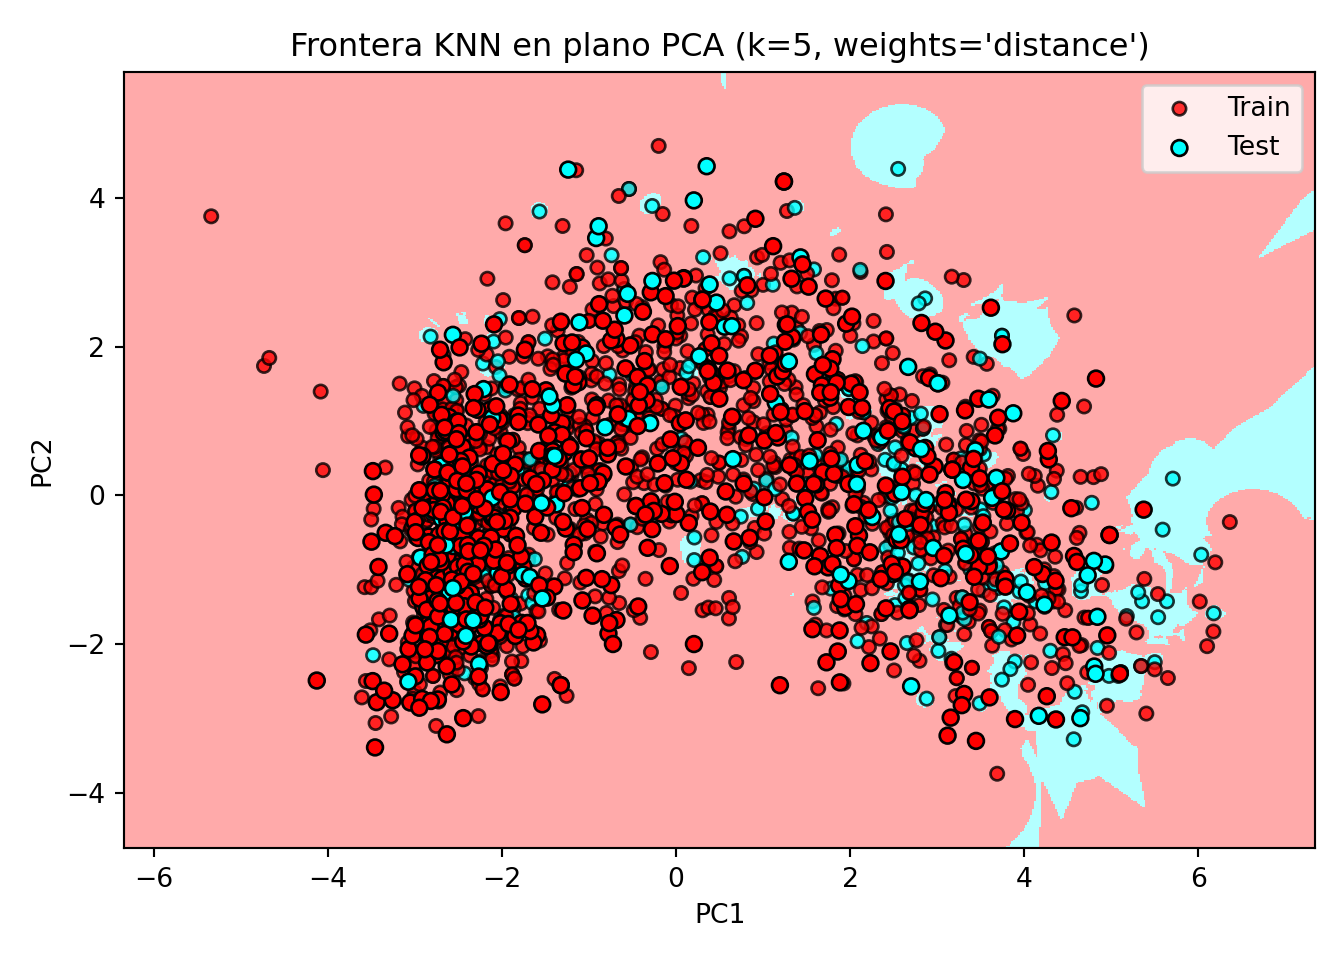
\includegraphics[keepaspectratio]{KnnNB_files/figure-pdf/grafico_clasificacion_python-3.pdf}}

\subsubsection{KNN Regresor}\label{knn-regresor}

\paragraph{Definimos los conjuntos de
datos}\label{definimos-los-conjuntos-de-datos-1}

\subsection{R: R base}

\begin{Shaded}
\begin{Highlighting}[]
\FunctionTok{library}\NormalTok{(FNN)}
\end{Highlighting}
\end{Shaded}

\begin{Shaded}
\begin{Highlighting}[]
\FunctionTok{set.seed}\NormalTok{(}\DecValTok{1994}\NormalTok{)}

\NormalTok{default\_idx }\OtherTok{=} \FunctionTok{sample}\NormalTok{(}\FunctionTok{nrow}\NormalTok{(datos), }\FunctionTok{nrow}\NormalTok{(datos)}\SpecialCharTok{*}\FloatTok{0.7}\NormalTok{)}

\NormalTok{datos }\OtherTok{\textless{}{-}}\NormalTok{ datos[, }\SpecialCharTok{{-}}\FunctionTok{c}\NormalTok{(}\DecValTok{1}\NormalTok{)]}

\NormalTok{train }\OtherTok{\textless{}{-}}\NormalTok{ datos[default\_idx, ]; test }\OtherTok{\textless{}{-}}\NormalTok{ datos[}\SpecialCharTok{{-}}\NormalTok{default\_idx, ]}
\NormalTok{X\_train }\OtherTok{\textless{}{-}}\NormalTok{ train[, }\SpecialCharTok{{-}}\DecValTok{6}\NormalTok{]; X\_test }\OtherTok{\textless{}{-}}\NormalTok{ test[, }\SpecialCharTok{{-}}\DecValTok{6}\NormalTok{]}
\NormalTok{y\_train }\OtherTok{\textless{}{-}}\NormalTok{ train[, }\DecValTok{6}\NormalTok{]; y\_test }\OtherTok{\textless{}{-}}\NormalTok{ test[, }\DecValTok{6}\NormalTok{]}

\CommentTok{\# Convertimos todas las columnas en numéricas para que se pueda utilizar el algoritmo}
\CommentTok{\# de KNN}
\NormalTok{X\_train }\OtherTok{\textless{}{-}} \FunctionTok{data.frame}\NormalTok{(}\FunctionTok{lapply}\NormalTok{(X\_train, as.numeric))}
\NormalTok{X\_test }\OtherTok{\textless{}{-}} \FunctionTok{data.frame}\NormalTok{(}\FunctionTok{lapply}\NormalTok{(X\_test, as.numeric))}
\end{Highlighting}
\end{Shaded}

\subsection{\texorpdfstring{R: packages
\texttt{caret}}{R: packages caret}}

\begin{Shaded}
\begin{Highlighting}[]
\FunctionTok{library}\NormalTok{(caret)}

\FunctionTok{set.seed}\NormalTok{(}\DecValTok{1994}\NormalTok{)}

\NormalTok{default\_idx }\OtherTok{\textless{}{-}} \FunctionTok{createDataPartition}\NormalTok{(datos}\SpecialCharTok{$}\NormalTok{Recency, }\AttributeTok{p =} \FloatTok{0.7}\NormalTok{, }\AttributeTok{list =} \ConstantTok{FALSE}\NormalTok{)}
\NormalTok{X\_trainC }\OtherTok{\textless{}{-}}\NormalTok{ datos[default\_idx, ]}
\NormalTok{X\_testC }\OtherTok{\textless{}{-}}\NormalTok{ datos[}\SpecialCharTok{{-}}\NormalTok{default\_idx, ]}
\NormalTok{y\_testC }\OtherTok{\textless{}{-}}\NormalTok{ X\_testC[, }\DecValTok{6}\NormalTok{]}
\end{Highlighting}
\end{Shaded}

\subsection{Python}

\begin{Shaded}
\begin{Highlighting}[]
\ImportTok{from}\NormalTok{ sklearn.model\_selection }\ImportTok{import}\NormalTok{ train\_test\_split}

\NormalTok{X }\OperatorTok{=}\NormalTok{ datos\_py.drop([}\StringTok{"Recency"}\NormalTok{], axis}\OperatorTok{=}\DecValTok{1}\NormalTok{)}
\NormalTok{y }\OperatorTok{=}\NormalTok{ datos\_py[}\StringTok{\textquotesingle{}Recency\textquotesingle{}}\NormalTok{]}

\NormalTok{X\_trainPy, X\_testPy, y\_trainPy, y\_testPy }\OperatorTok{=}\NormalTok{ train\_test\_split(X, y, test\_size }\OperatorTok{=} \FloatTok{0.3}\NormalTok{, random\_state }\OperatorTok{=} \DecValTok{1994}\NormalTok{)}

\ImportTok{from}\NormalTok{ sklearn.compose }\ImportTok{import}\NormalTok{ ColumnTransformer}
\ImportTok{from}\NormalTok{ sklearn.preprocessing }\ImportTok{import}\NormalTok{ OneHotEncoder, StandardScaler}
\ImportTok{from}\NormalTok{ sklearn.pipeline }\ImportTok{import}\NormalTok{ Pipeline}

\CommentTok{\# y para regresión debe ser numérico:}
\NormalTok{y\_train }\OperatorTok{=}\NormalTok{ np.asarray(y\_trainPy, dtype}\OperatorTok{=}\BuiltInTok{float}\NormalTok{)}
\NormalTok{y\_test  }\OperatorTok{=}\NormalTok{ np.asarray(y\_testPy,  dtype}\OperatorTok{=}\BuiltInTok{float}\NormalTok{)}

\CommentTok{\# Detecta tipos}
\NormalTok{num\_cols }\OperatorTok{=}\NormalTok{ X\_trainPy.select\_dtypes(include}\OperatorTok{=}\NormalTok{[np.number]).columns.tolist()}
\NormalTok{cat\_cols }\OperatorTok{=}\NormalTok{ X\_trainPy.select\_dtypes(exclude}\OperatorTok{=}\NormalTok{[np.number]).columns.tolist()}

\CommentTok{\# Preprocesador: escala numéricas y one{-}hot en categóricas}
\NormalTok{preprocess }\OperatorTok{=}\NormalTok{ ColumnTransformer(}
\NormalTok{    transformers}\OperatorTok{=}\NormalTok{[}
\NormalTok{        (}\StringTok{"num"}\NormalTok{, StandardScaler(), num\_cols),}
\NormalTok{        (}\StringTok{"cat"}\NormalTok{, OneHotEncoder(handle\_unknown}\OperatorTok{=}\StringTok{"ignore"}\NormalTok{, sparse\_output}\OperatorTok{=}\VariableTok{False}\NormalTok{), cat\_cols),}
\NormalTok{    ],}
\NormalTok{    remainder}\OperatorTok{=}\StringTok{"drop"}
\NormalTok{)}

\CommentTok{\# Transforma los datos usando el preprocesador ya ajustado}
\NormalTok{X\_trainPy }\OperatorTok{=}\NormalTok{ preprocess.fit\_transform(X\_trainPy)}
\NormalTok{X\_testPy  }\OperatorTok{=}\NormalTok{ preprocess.transform(X\_testPy)}
\end{Highlighting}
\end{Shaded}

\paragraph{Entrenamiento del modelo}\label{entrenamiento-del-modelo-1}

\subsection{R: R base}

\begin{Shaded}
\begin{Highlighting}[]
\NormalTok{pred }\OtherTok{\textless{}{-}} \FunctionTok{knn.reg}\NormalTok{(}\AttributeTok{train =}\NormalTok{ X\_train, }\AttributeTok{test =}\NormalTok{ X\_test, }\AttributeTok{y =}\NormalTok{ y\_train, }\AttributeTok{k =} \DecValTok{1}\NormalTok{)}
\FunctionTok{head}\NormalTok{(pred)}
\end{Highlighting}
\end{Shaded}

\begin{verbatim}
$call
knn.reg(train = X_train, test = X_test, y = y_train, k = 1)

$k
[1] 1

$n
[1] 665

$pred
  [1] 171  14 102  32 469  14  38  67  64 171   2  43 746 217  17  69 818 333
 [19]   1 222 223  11  22 711  42 483  38   3  31 300  44  81  21  50  45 319
 [37] 352  31  42  62  24  24 115 300   6 117   8 223  16   5 186  90  13 168
 [55]  35   6  56   5  40   4 345 300  61 194  38 717 226  58  58   5  24  30
 [73] 168  27 145 689 107  67  16  50  44  70 100  21  46  92 431 178 570 161
 [91] 292   5  10  99  26 348  71  50 597  26 252  18   7  13  13 132  21 694
[109]  30  24  17  24   8   8 141  14   8  14 175 115 161  13   3  69 320 185
[127] 215  13  16  13  63 128 189  24 860  39 417  97   2 689  13   4  26 194
[145] 199 364   4 860 215 195 119 507  73  27 142   5  28  11 711  75 172  92
[163]  10  12 267 929  12   6   3 101  65  22 161 129 129   3  30   2 561 129
[181]  29  47 108  92  11   2 384  83  11 249  46  44  24 217 294  18 212   8
[199]   8 128   2 178 501 127 132 119 413 559  11 704 843  50  46 137  22 137
[217]   3  35  10   4   7  69 929  11  19  10  92   7  31 568  47 243 424 689
[235]   8  14 130 212  31  15 420 395  40  49 706  50 107 142 108 333  50   7
[253]   8  22  18 132  50 535   8   6 226   8  14   5 275  83 119 119   5 845
[271]  23  57  17   6  27  21  59 154   4   5  40 746 746  39  43   5 204 295
[289]  13 264 132  83 107 160   4   5  17  81 205  16   6 305 305 845 107  18
[307]  92  65 238  18 253 169  18 194 292  50  15  64   2 100 100  85 746  98
[325]  11  32  46  29  81 317 259   8   3  10  46  84  18 237  10  13  29  75
[343]  29 639  17  27  60  89  18  10 189 123  11  51 864   4   7  29   7  16
[361]   3  29 594  17  29 445   3  27  17 206 913  97 377  22   9  21  84  11
[379]  16 149  10  10   4  51 238 238 345 171  30  76  16 215   5  13 493 403
[397] 128 107  21 444 756 104 104 345 345  57  27  49 298 352  12 131 216   7
[415]  20 154  28 217 160  10  13  14  31  44 403 403 128 137  64 294  14 925
[433]  74 790  19   7   5 590 590  33 142 217   5 101  93 100 180   8  46  93
[451]  15   1   6 247  64   3 140  93   8  10  21 257 697  19  72  15  14 109
[469]  93 124   6 108 462 568  83  10  29 160   6 465  74  14  14  66  71   7
[487] 756  20 567  85 183  12  76 112 690 168 179 140  56   5  26 309 128  11
[505] 137  13  15  11  54  54  16 151  24 387 133   9  16  27  30 324 287   7
[523]  12 170  15  12  24 430  30  24 114 447 129  25  25  28 239  92   7  18
[541]   5 612 154  10  22 168  73 368  15  11   5 253  76 287 112 217 133  19
[559]   3  60 329   7  25 815  73 487  14 135  15   9  19   2 264  63  63 936
[577]  16  79 359  88 415  65 792 387 449  11  12 278 221  10 534 428  18  19
[595]  63   2  11 213  17 387  24  48 159   7   7   3  60  19 430  23  19 113
[613]   9  46  54  41  21 500 103  74 597  23 420  39  25   4  14  43 106  33
[631]  55 103  20 363 217  21  19 110   3  15 103  10   5 414  14  14 255  99
[649]  22 159  19   3 838 818  15  11 128 838   6  24 142   3  21 159 500

$residuals
NULL

$PRESS
NULL
\end{verbatim}

\subsection{\texorpdfstring{R: packages
\texttt{caret}}{R: packages caret}}

\begin{Shaded}
\begin{Highlighting}[]
\NormalTok{caret}\SpecialCharTok{::}\FunctionTok{modelLookup}\NormalTok{(}\StringTok{"knn"}\NormalTok{)}
\end{Highlighting}
\end{Shaded}

\begin{verbatim}
  model parameter      label forReg forClass probModel
1   knn         k #Neighbors   TRUE     TRUE      TRUE
\end{verbatim}

\begin{Shaded}
\begin{Highlighting}[]
\NormalTok{knn }\OtherTok{\textless{}{-}} \FunctionTok{train}\NormalTok{(Recency }\SpecialCharTok{\textasciitilde{}}\NormalTok{ ., }\AttributeTok{data =}\NormalTok{ X\_trainC, }\AttributeTok{method =} \StringTok{"knn"}\NormalTok{,}
             \AttributeTok{preProc =} \FunctionTok{c}\NormalTok{(}\StringTok{"center"}\NormalTok{, }\StringTok{"scale"}\NormalTok{), }\AttributeTok{tuneGrid =} \FunctionTok{data.frame}\NormalTok{(}\AttributeTok{k =} \DecValTok{1}\SpecialCharTok{:}\DecValTok{10}\NormalTok{),}
             \AttributeTok{trControl =} \FunctionTok{trainControl}\NormalTok{(}\AttributeTok{method =} \StringTok{"cv"}\NormalTok{, }\AttributeTok{number =} \DecValTok{10}\NormalTok{))}

\FunctionTok{ggplot}\NormalTok{(knn, }\AttributeTok{highlight =} \ConstantTok{TRUE}\NormalTok{) }\CommentTok{\# Alternativamente: plot(knn)}
\end{Highlighting}
\end{Shaded}

\pandocbounded{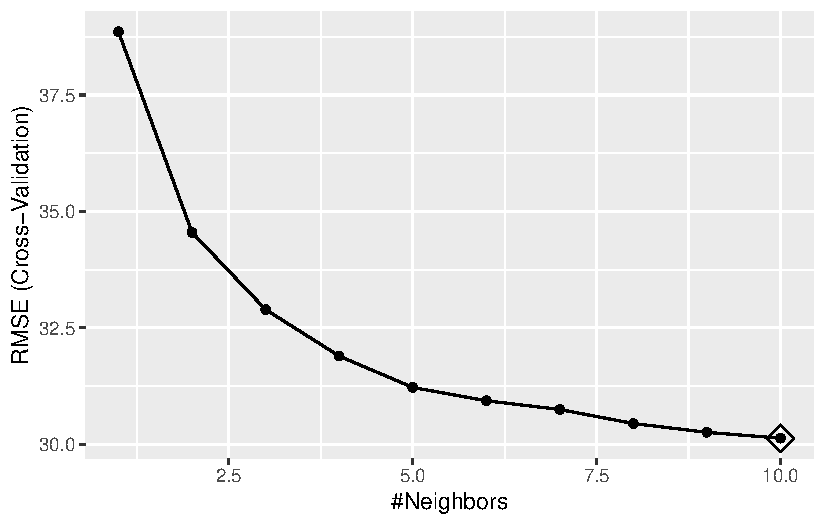
\includegraphics[keepaspectratio]{KnnNB_files/figure-pdf/training_caret_regresion-1.pdf}}

\subsection{Python}

\begin{Shaded}
\begin{Highlighting}[]
\ImportTok{from}\NormalTok{ sklearn.neighbors }\ImportTok{import}\NormalTok{ KNeighborsRegressor}
\ImportTok{from}\NormalTok{ sklearn.metrics }\ImportTok{import}\NormalTok{ mean\_squared\_error, r2\_score}

\CommentTok{\# Create and train the KNN regressor}
\NormalTok{knn\_regressor }\OperatorTok{=}\NormalTok{ KNeighborsRegressor(n\_neighbors }\OperatorTok{=} \DecValTok{5}\NormalTok{)}
\NormalTok{knn\_regressor.fit(X\_trainPy, y\_trainPy)}
\end{Highlighting}
\end{Shaded}

\begin{verbatim}
KNeighborsRegressor()
\end{verbatim}

\paragraph{\texorpdfstring{\textbf{Tunning parameters:} Selección del
valor de
k}{Tunning parameters: Selección del valor de k}}\label{tunning-parameters-selecciuxf3n-del-valor-de-k-1}

\subsection{R: R base}

\begin{Shaded}
\begin{Highlighting}[]
\NormalTok{rmse }\OtherTok{=} \ControlFlowTok{function}\NormalTok{(actual, predicted) \{}
  \FunctionTok{sqrt}\NormalTok{(}\FunctionTok{mean}\NormalTok{((actual }\SpecialCharTok{{-}}\NormalTok{ predicted) }\SpecialCharTok{\^{}} \DecValTok{2}\NormalTok{))}
\NormalTok{\}}

\CommentTok{\# define helper function for getting knn.reg predictions}
\CommentTok{\# note: this function is highly specific to this situation and dataset}
\NormalTok{make\_knn\_pred }\OtherTok{\textless{}{-}} \ControlFlowTok{function}\NormalTok{(}\AttributeTok{k =} \DecValTok{1}\NormalTok{, training, predicting, valueTarget) \{}
\NormalTok{  pred }\OtherTok{=}\NormalTok{ FNN}\SpecialCharTok{::}\FunctionTok{knn.reg}\NormalTok{(}\AttributeTok{train =}\NormalTok{ training, }
                      \AttributeTok{test =}\NormalTok{ predicting, }
                      \AttributeTok{y =}\NormalTok{ valueTarget, }\AttributeTok{k =}\NormalTok{ k)}\SpecialCharTok{$}\NormalTok{pred}
\NormalTok{  act  }\OtherTok{=}\NormalTok{ predicting}\SpecialCharTok{$}\NormalTok{Recency}
  \FunctionTok{rmse}\NormalTok{(}\AttributeTok{predicted =}\NormalTok{ pred, }\AttributeTok{actual =}\NormalTok{ act)}
\NormalTok{\}}
\end{Highlighting}
\end{Shaded}

\begin{Shaded}
\begin{Highlighting}[]
\CommentTok{\# define values of k to evaluate}
\NormalTok{k }\OtherTok{=} \FunctionTok{c}\NormalTok{(}\DecValTok{1}\NormalTok{, }\DecValTok{5}\NormalTok{, }\DecValTok{10}\NormalTok{, }\DecValTok{25}\NormalTok{, }\DecValTok{50}\NormalTok{, }\DecValTok{250}\NormalTok{)}

\CommentTok{\# get requested train RMSEs}
\NormalTok{knn\_trn\_rmse }\OtherTok{\textless{}{-}} \FunctionTok{sapply}\NormalTok{(k, make\_knn\_pred, }\AttributeTok{training =}\NormalTok{ X\_train, }
                      \AttributeTok{predicting =}\NormalTok{ X\_train, }
                      \AttributeTok{valueTarget =}\NormalTok{ y\_train)}

\CommentTok{\# determine "best" k}
\NormalTok{best\_k }\OtherTok{\textless{}{-}}\NormalTok{ k[}\FunctionTok{which.min}\NormalTok{(knn\_trn\_rmse)]}
\end{Highlighting}
\end{Shaded}

\subsection{\texorpdfstring{R: packages
\texttt{caret}}{R: packages caret}}

\begin{Shaded}
\begin{Highlighting}[]
\NormalTok{regSummary }\OtherTok{\textless{}{-}} \ControlFlowTok{function}\NormalTok{(data, }\AttributeTok{lev =} \ConstantTok{NULL}\NormalTok{, }\AttributeTok{model =} \ConstantTok{NULL}\NormalTok{) \{}
\NormalTok{  out }\OtherTok{\textless{}{-}} \FunctionTok{c}\NormalTok{(}
    \AttributeTok{RMSE =} \FunctionTok{RMSE}\NormalTok{(data}\SpecialCharTok{$}\NormalTok{pred, data}\SpecialCharTok{$}\NormalTok{obs),}
    \AttributeTok{Rsquared =} \FunctionTok{R2}\NormalTok{(data}\SpecialCharTok{$}\NormalTok{pred, data}\SpecialCharTok{$}\NormalTok{obs),}
    \AttributeTok{MAE =} \FunctionTok{MAE}\NormalTok{(data}\SpecialCharTok{$}\NormalTok{pred, data}\SpecialCharTok{$}\NormalTok{obs)}
\NormalTok{  )}
\NormalTok{  out}
\NormalTok{\}}

\CommentTok{\# Definimos un método de remuestreo}
\NormalTok{cv }\OtherTok{\textless{}{-}} \FunctionTok{trainControl}\NormalTok{(}
  \AttributeTok{method =} \StringTok{"repeatedcv"}\NormalTok{,}
  \AttributeTok{number =} \DecValTok{10}\NormalTok{,}
  \AttributeTok{repeats =} \DecValTok{5}\NormalTok{,}
  \AttributeTok{classProbs =} \ConstantTok{TRUE}\NormalTok{,}
  \AttributeTok{preProcOptions =} \FunctionTok{list}\NormalTok{(}\StringTok{"center"}\NormalTok{),}
  \AttributeTok{summaryFunction =}\NormalTok{ regSummary, }
  \AttributeTok{savePredictions =} \StringTok{"final"}\NormalTok{)}

\CommentTok{\# Definimos la red de posibles valores del hiperparámetro}
\NormalTok{hyper\_grid }\OtherTok{\textless{}{-}} \FunctionTok{expand.grid}\NormalTok{(}\AttributeTok{k =} \FunctionTok{c}\NormalTok{(}\DecValTok{1}\SpecialCharTok{:}\DecValTok{10}\NormalTok{,}\DecValTok{15}\NormalTok{,}\DecValTok{20}\NormalTok{,}\DecValTok{30}\NormalTok{,}\DecValTok{50}\NormalTok{,}\DecValTok{75}\NormalTok{,}\DecValTok{100}\NormalTok{))}
\end{Highlighting}
\end{Shaded}

\begin{Shaded}
\begin{Highlighting}[]
\FunctionTok{set.seed}\NormalTok{(}\DecValTok{1994}\NormalTok{)}

\CommentTok{\# Se entrena el modelo ajustando el hiperparámetro óptimo}
\NormalTok{model }\OtherTok{\textless{}{-}} \FunctionTok{train}\NormalTok{(}
\NormalTok{  Recency }\SpecialCharTok{\textasciitilde{}}\NormalTok{ .,}
  \AttributeTok{data =}\NormalTok{ X\_trainC,}
  \AttributeTok{method =} \StringTok{"knn"}\NormalTok{,}
  \AttributeTok{trControl =}\NormalTok{ cv,}
  \AttributeTok{tuneGrid =}\NormalTok{ hyper\_grid,}
  \AttributeTok{metric =} \StringTok{"MAPE"}\NormalTok{)}
\end{Highlighting}
\end{Shaded}

\subsection{Python}

\begin{Shaded}
\begin{Highlighting}[]
\ImportTok{import}\NormalTok{ matplotlib.pyplot }\ImportTok{as}\NormalTok{ plt }\CommentTok{\# for data visualization purposes}

\KeywordTok{def}\NormalTok{ mean\_absolute\_percentage\_error(y\_true, y\_pred):}
\NormalTok{    y\_true, y\_pred }\OperatorTok{=}\NormalTok{ np.array(y\_true), np.array(y\_pred)}
    \CommentTok{\# Evitar divisiones por cero}
\NormalTok{    mask }\OperatorTok{=}\NormalTok{ y\_true }\OperatorTok{!=} \DecValTok{0}
    \ControlFlowTok{return}\NormalTok{ np.mean(np.}\BuiltInTok{abs}\NormalTok{((y\_true[mask] }\OperatorTok{{-}}\NormalTok{ y\_pred[mask]) }\OperatorTok{/}\NormalTok{ y\_true[mask])) }\OperatorTok{*} \DecValTok{100}

\NormalTok{k\_range }\OperatorTok{=} \BuiltInTok{range}\NormalTok{(}\DecValTok{1}\NormalTok{, }\DecValTok{20}\NormalTok{)}
\NormalTok{scores }\OperatorTok{=}\NormalTok{ []}

\ControlFlowTok{for}\NormalTok{ k }\KeywordTok{in}\NormalTok{ k\_range:}
\NormalTok{    knn }\OperatorTok{=}\NormalTok{ KNeighborsRegressor(n\_neighbors}\OperatorTok{=}\NormalTok{k)}
\NormalTok{    knn.fit(X\_trainPy, y\_trainPy)}
\NormalTok{    y\_pred }\OperatorTok{=}\NormalTok{ knn.predict(X\_testPy)}
\NormalTok{    mape }\OperatorTok{=}\NormalTok{ mean\_absolute\_percentage\_error(y\_testPy, y\_pred)}
\NormalTok{    scores.append(mape)}
\end{Highlighting}
\end{Shaded}

\begin{verbatim}
KNeighborsRegressor(n_neighbors=1)
KNeighborsRegressor(n_neighbors=2)
KNeighborsRegressor(n_neighbors=3)
KNeighborsRegressor(n_neighbors=4)
KNeighborsRegressor()
KNeighborsRegressor(n_neighbors=6)
KNeighborsRegressor(n_neighbors=7)
KNeighborsRegressor(n_neighbors=8)
KNeighborsRegressor(n_neighbors=9)
KNeighborsRegressor(n_neighbors=10)
KNeighborsRegressor(n_neighbors=11)
KNeighborsRegressor(n_neighbors=12)
KNeighborsRegressor(n_neighbors=13)
KNeighborsRegressor(n_neighbors=14)
KNeighborsRegressor(n_neighbors=15)
KNeighborsRegressor(n_neighbors=16)
KNeighborsRegressor(n_neighbors=17)
KNeighborsRegressor(n_neighbors=18)
KNeighborsRegressor(n_neighbors=19)
\end{verbatim}

\begin{Shaded}
\begin{Highlighting}[]
\NormalTok{plt.figure(figsize}\OperatorTok{=}\NormalTok{(}\DecValTok{6}\NormalTok{,}\DecValTok{4}\NormalTok{))}
\NormalTok{plt.plot(k\_range, scores, marker}\OperatorTok{=}\StringTok{\textquotesingle{}o\textquotesingle{}}\NormalTok{)}
\NormalTok{plt.xlabel(}\StringTok{\textquotesingle{}k\textquotesingle{}}\NormalTok{)}
\NormalTok{plt.ylabel(}\StringTok{\textquotesingle{}MAPE (\%)\textquotesingle{}}\NormalTok{)}
\NormalTok{plt.title(}\StringTok{\textquotesingle{}Error porcentual medio absoluto vs número de vecinos (k)\textquotesingle{}}\NormalTok{)}
\NormalTok{plt.xticks([}\DecValTok{0}\NormalTok{,}\DecValTok{5}\NormalTok{,}\DecValTok{10}\NormalTok{,}\DecValTok{15}\NormalTok{,}\DecValTok{20}\NormalTok{])}
\end{Highlighting}
\end{Shaded}

\begin{verbatim}
([<matplotlib.axis.XTick object at 0x0000024CE182DB90>, <matplotlib.axis.XTick object at 0x0000024CE19A2390>, <matplotlib.axis.XTick object at 0x0000024CF2CDE210>, <matplotlib.axis.XTick object at 0x0000024CF2CDF3D0>, <matplotlib.axis.XTick object at 0x0000024CF2CEAE10>], [Text(0, 0, '0'), Text(5, 0, '5'), Text(10, 0, '10'), Text(15, 0, '15'), Text(20, 0, '20')])
\end{verbatim}

\begin{Shaded}
\begin{Highlighting}[]
\NormalTok{plt.show()}
\end{Highlighting}
\end{Shaded}

\pandocbounded{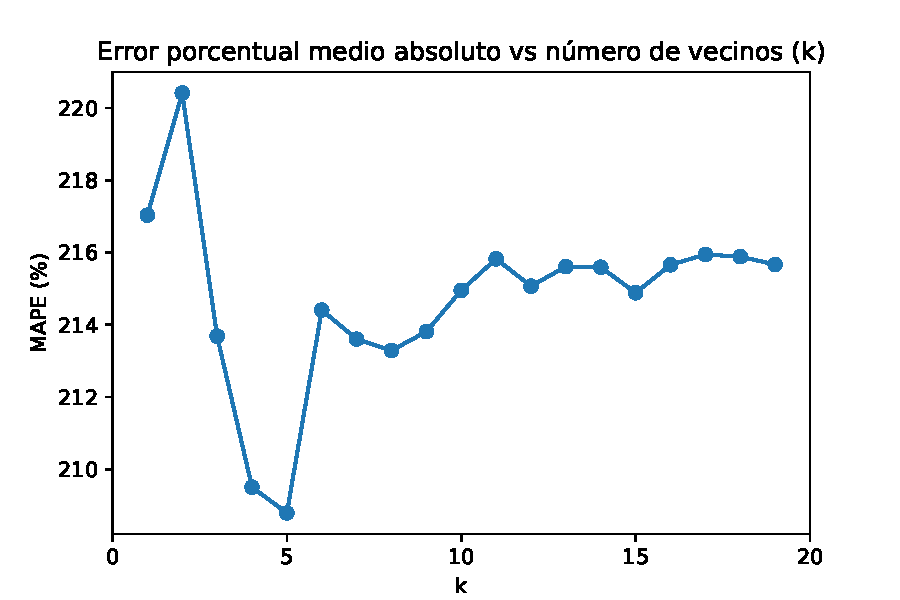
\includegraphics[keepaspectratio]{KnnNB_files/figure-pdf/entrenamiento_cv_python-1.pdf}}

\paragraph{Predicción de la variable
respuesta}\label{predicciuxf3n-de-la-variable-respuesta-1}

\subsection{R: R base}

La própia función que entrena el algoritmo ya devuelve las predicciones
del algoritmo de KNN.

\subsection{\texorpdfstring{R: packages
\texttt{caret}}{R: packages caret}}

\begin{Shaded}
\begin{Highlighting}[]
\FunctionTok{head}\NormalTok{(}\FunctionTok{predict}\NormalTok{(model, }\AttributeTok{newdata =}\NormalTok{ X\_testC), }\AttributeTok{n =} \DecValTok{10}\NormalTok{)}
\end{Highlighting}
\end{Shaded}

\begin{verbatim}
 [1] 53.42667 45.97333 45.33333 45.33333 49.16000 50.50667 42.37333 51.86667
 [9] 41.64474 45.14667
\end{verbatim}

\subsection{Python}

\begin{Shaded}
\begin{Highlighting}[]
\NormalTok{y\_predPy }\OperatorTok{=}\NormalTok{ knn\_regressor.predict(X\_testPy)}
\NormalTok{y\_predPy[:}\DecValTok{10}\NormalTok{]}
\end{Highlighting}
\end{Shaded}

\begin{verbatim}
array([59.8, 56.4, 52. , 30.6, 24.6, 64.2, 48.8, 19.8, 56.6, 44. ])
\end{verbatim}

\subsection{\texorpdfstring{Naives Bayes
(\emph{Classifier})}{Naives Bayes (Classifier)}}\label{naives-bayes-classifier}

\subsubsection{Definición de los conjuntos de
datos}\label{definiciuxf3n-de-los-conjuntos-de-datos}

\subsection{R: R Base}

\begin{Shaded}
\begin{Highlighting}[]
\FunctionTok{set.seed}\NormalTok{(}\DecValTok{1994}\NormalTok{)}

\NormalTok{ind\_col }\OtherTok{\textless{}{-}} \FunctionTok{c}\NormalTok{(}\DecValTok{16}\NormalTok{)}

\NormalTok{default\_idx }\OtherTok{=} \FunctionTok{sample}\NormalTok{(}\FunctionTok{nrow}\NormalTok{(datos), }\FunctionTok{nrow}\NormalTok{(datos)}\SpecialCharTok{*}\FloatTok{0.7}\NormalTok{)}
\NormalTok{train }\OtherTok{\textless{}{-}}\NormalTok{ datos[default\_idx, ]; test }\OtherTok{\textless{}{-}}\NormalTok{ datos[}\SpecialCharTok{{-}}\NormalTok{default\_idx, ]}
\NormalTok{X\_train }\OtherTok{\textless{}{-}}\NormalTok{ train; }
\CommentTok{\# X\_train \textless{}{-} train[, {-}ind\_col];}
\NormalTok{X\_test }\OtherTok{\textless{}{-}}\NormalTok{ test[, }\SpecialCharTok{{-}}\NormalTok{ind\_col]}
\NormalTok{y\_train }\OtherTok{\textless{}{-}}\NormalTok{ train[, ind\_col]; y\_test }\OtherTok{\textless{}{-}}\NormalTok{ test[, ind\_col]}

\CommentTok{\# Convertimos todas las columnas en numéricas para que se pueda utilizar el algoritmo}
\CommentTok{\# de KNN}
\CommentTok{\# X\_train \textless{}{-} data.frame(lapply(X\_train, as.numeric))}
\CommentTok{\# X\_test \textless{}{-} data.frame(lapply(X\_test, as.numeric))}
\end{Highlighting}
\end{Shaded}

\subsection{\texorpdfstring{R: Packages
\texttt{caret}}{R: Packages caret}}

\begin{Shaded}
\begin{Highlighting}[]
\FunctionTok{library}\NormalTok{(}\StringTok{"caret"}\NormalTok{)}
\FunctionTok{library}\NormalTok{(}\StringTok{"naivebayes"}\NormalTok{)}
\FunctionTok{library}\NormalTok{(}\StringTok{"reshape"}\NormalTok{)}
\FunctionTok{library}\NormalTok{(}\StringTok{"ggplot2"}\NormalTok{)}

\FunctionTok{set.seed}\NormalTok{(}\DecValTok{1994}\NormalTok{)}

\NormalTok{ind\_col }\OtherTok{\textless{}{-}} \FunctionTok{c}\NormalTok{(}\DecValTok{16}\NormalTok{)}
\NormalTok{default\_idx }\OtherTok{\textless{}{-}} \FunctionTok{createDataPartition}\NormalTok{(datos}\SpecialCharTok{$}\NormalTok{Response, }\AttributeTok{p =} \FloatTok{0.7}\NormalTok{, }\AttributeTok{list =} \ConstantTok{FALSE}\NormalTok{)}
\NormalTok{X\_trainC }\OtherTok{\textless{}{-}}\NormalTok{ datos[default\_idx, ]}
\NormalTok{X\_testC }\OtherTok{\textless{}{-}}\NormalTok{ datos[}\SpecialCharTok{{-}}\NormalTok{default\_idx, ]}
\NormalTok{y\_testC }\OtherTok{\textless{}{-}}\NormalTok{ X\_testC[, ind\_col]}
\NormalTok{X\_testC }\OtherTok{\textless{}{-}}\NormalTok{ X\_testC[, }\SpecialCharTok{{-}}\NormalTok{ind\_col]}
\end{Highlighting}
\end{Shaded}

\begin{Shaded}
\begin{Highlighting}[]
\FunctionTok{modelLookup}\NormalTok{(}\StringTok{"naive\_bayes"}\NormalTok{)}
\end{Highlighting}
\end{Shaded}

\begin{verbatim}
        model parameter                label forReg forClass probModel
1 naive_bayes   laplace   Laplace Correction  FALSE     TRUE      TRUE
2 naive_bayes usekernel    Distribution Type  FALSE     TRUE      TRUE
3 naive_bayes    adjust Bandwidth Adjustment  FALSE     TRUE      TRUE
\end{verbatim}

\subsection{Python}

\begin{Shaded}
\begin{Highlighting}[]
\ImportTok{from}\NormalTok{ sklearn.model\_selection }\ImportTok{import}\NormalTok{ train\_test\_split}

\NormalTok{X }\OperatorTok{=}\NormalTok{ datos\_py.drop([}\StringTok{"Response"}\NormalTok{], axis}\OperatorTok{=}\DecValTok{1}\NormalTok{)}
\NormalTok{y }\OperatorTok{=}\NormalTok{ datos\_py[}\StringTok{\textquotesingle{}Response\textquotesingle{}}\NormalTok{]}

\NormalTok{X\_trainPy, X\_testPy, y\_trainPy, y\_testPy }\OperatorTok{=}\NormalTok{ train\_test\_split(X, y, test\_size }\OperatorTok{=} \FloatTok{0.3}\NormalTok{, random\_state }\OperatorTok{=} \DecValTok{1994}\NormalTok{)}
\end{Highlighting}
\end{Shaded}

\subsubsection{Entrenamiento del
modelo}\label{entrenamiento-del-modelo-2}

\subsection{R: R base}

\begin{Shaded}
\begin{Highlighting}[]
\FunctionTok{library}\NormalTok{(e1071)}

\NormalTok{(nb\_base }\OtherTok{\textless{}{-}} \FunctionTok{naiveBayes}\NormalTok{(Response }\SpecialCharTok{\textasciitilde{}}\NormalTok{ ., }\AttributeTok{data =}\NormalTok{ X\_train))}
\end{Highlighting}
\end{Shaded}

\begin{verbatim}

Naive Bayes Classifier for Discrete Predictors

Call:
naiveBayes.default(x = X, y = Y, laplace = laplace)

A-priori probabilities:
Y
       No       Yes 
0.8523533 0.1476467 

Conditional probabilities:
     Kidhome
Y          [,1]      [,2]
  No  0.4349470 0.5383867
  Yes 0.3799127 0.5041390

     Teenhome
Y          [,1]      [,2]
  No  0.5378215 0.5437755
  Yes 0.2969432 0.4857977

     Recency
Y         [,1]     [,2]
  No  51.97731 28.59796
  Yes 34.79476 27.41649

     MntWines
Y         [,1]     [,2]
  No  274.1944 303.7532
  Yes 491.6987 425.0553

     MntFruits
Y         [,1]     [,2]
  No  25.40847 39.46007
  Yes 38.14410 46.63587

     MntMeatProducts
Y         [,1]     [,2]
  No  150.5719 210.0253
  Yes 289.3406 288.9687

     MntFishProducts
Y         [,1]     [,2]
  No  35.83888 53.15100
  Yes 53.18341 64.71829

     MntSweetProducts
Y         [,1]     [,2]
  No  26.44781 40.62991
  Yes 41.91266 50.01554

     MntGoldProds
Y         [,1]     [,2]
  No  41.22617 49.78208
  Yes 58.64192 56.85865

     NumDealsPurchases
Y         [,1]     [,2]
  No  2.274584 1.841840
  Yes 2.305677 2.078084

     NumWebPurchases
Y         [,1]     [,2]
  No  3.925870 2.684626
  Yes 4.982533 2.630731

     NumCatalogPurchases
Y         [,1]     [,2]
  No  2.472769 2.870076
  Yes 4.283843 3.201254

     NumStorePurchases
Y         [,1]     [,2]
  No  5.806354 3.278682
  Yes 6.213974 3.247479

     NumWebVisitsMonth
Y         [,1]     [,2]
  No  5.245083 2.443703
  Yes 5.275109 2.655405

     Edad
Y         [,1]     [,2]
  No  56.27837 12.05355
  Yes 54.92576 12.28602

     Education_Basic
Y            [,1]       [,2]
  No  0.027231467 0.16281882
  Yes 0.008733624 0.09324869

     Education_Graduation
Y          [,1]      [,2]
  No  0.5136157 0.5000037
  Yes 0.4454148 0.4981003

     Education_Master
Y          [,1]      [,2]
  No  0.1641452 0.3705475
  Yes 0.1441048 0.3519653

     Education_PhD
Y          [,1]      [,2]
  No  0.2027231 0.4021801
  Yes 0.3231441 0.4687017

     Marital_Status_Alone
Y             [,1]       [,2]
  No  0.0007564297 0.02750327
  Yes 0.0043668122 0.06608186

     Marital_Status_Divorced
Y           [,1]      [,2]
  No  0.09077156 0.2873927
  Yes 0.15283843 0.3606199

     Marital_Status_Married
Y          [,1]      [,2]
  No  0.4054463 0.4911640
  Yes 0.3100437 0.4635243

     Marital_Status_Single
Y          [,1]      [,2]
  No  0.1891074 0.3917421
  Yes 0.3144105 0.4652977

     Marital_Status_Together
Y          [,1]      [,2]
  No  0.2813918 0.4498484
  Yes 0.1659389 0.3728407

     Marital_Status_Widow
Y           [,1]      [,2]
  No  0.03101362 0.1734201
  Yes 0.04803493 0.2143085

     Marital_Status_YOLO
Y             [,1]       [,2]
  No  0.0007564297 0.02750327
  Yes 0.0000000000 0.00000000

     mes_cliente_2
Y              0          1
  No  0.91527988 0.08472012
  Yes 0.90829694 0.09170306

     mes_cliente_3
Y              0          1
  No  0.90544629 0.09455371
  Yes 0.92576419 0.07423581

     mes_cliente_4
Y              0          1
  No  0.91830560 0.08169440
  Yes 0.91266376 0.08733624

     mes_cliente_5
Y              0          1
  No  0.90922844 0.09077156
  Yes 0.95633188 0.04366812

     mes_cliente_6
Y              0          1
  No  0.91906203 0.08093797
  Yes 0.92576419 0.07423581

     mes_cliente_7
Y              0          1
  No  0.93948563 0.06051437
  Yes 0.93886463 0.06113537

     mes_cliente_8
Y              0          1
  No  0.90771558 0.09228442
  Yes 0.89956332 0.10043668

     mes_cliente_9
Y              0          1
  No  0.93267776 0.06732224
  Yes 0.90829694 0.09170306

     mes_cliente_10
Y              0          1
  No  0.91301059 0.08698941
  Yes 0.86462882 0.13537118

     mes_cliente_11
Y              0          1
  No  0.91981846 0.08018154
  Yes 0.92576419 0.07423581

     mes_cliente_12
Y              0          1
  No  0.90771558 0.09228442
  Yes 0.92576419 0.07423581

     Complain_Yes
Y           [,1]      [,2]
  No  0.01059002 0.1024002
  Yes 0.01310044 0.1139540
\end{verbatim}

\subsection{\texorpdfstring{R: Packages
\texttt{caret}}{R: Packages caret}}

\begin{Shaded}
\begin{Highlighting}[]
\CommentTok{\# se fija la semilla aleatoria}
\FunctionTok{set.seed}\NormalTok{(}\DecValTok{1994}\NormalTok{)}

\CommentTok{\# se entrena el modelo}
\NormalTok{model }\OtherTok{\textless{}{-}} \FunctionTok{train}\NormalTok{(Response }\SpecialCharTok{\textasciitilde{}}\NormalTok{ .,}
            \AttributeTok{data=}\NormalTok{X\_trainC,}
            \AttributeTok{method=}\StringTok{"nb"}\NormalTok{,}
            \AttributeTok{metric=}\StringTok{"Accuracy"}\NormalTok{,}
            \AttributeTok{trControl=}\FunctionTok{trainControl}\NormalTok{(}\AttributeTok{classProbs =} \ConstantTok{TRUE}\NormalTok{,}
                                   \AttributeTok{method =} \StringTok{"cv"}\NormalTok{,}
                                   \AttributeTok{number =} \DecValTok{10}\NormalTok{))}

\CommentTok{\# se muestra la salida del modelo}
\NormalTok{model}
\end{Highlighting}
\end{Shaded}

\begin{verbatim}
Naive Bayes 

1553 samples
  38 predictor
   2 classes: 'No', 'Yes' 

No pre-processing
Resampling: Cross-Validated (10 fold) 
Summary of sample sizes: 1397, 1398, 1397, 1397, 1398, 1398, ... 
Resampling results across tuning parameters:

  usekernel  Accuracy  Kappa   
  FALSE           NaN       NaN
   TRUE      0.845491  0.237876

Tuning parameter 'fL' was held constant at a value of 0
Tuning
 parameter 'adjust' was held constant at a value of 1
Accuracy was used to select the optimal model using the largest value.
The final values used for the model were fL = 0, usekernel = TRUE and adjust
 = 1.
\end{verbatim}

\subsection{Python}

\begin{Shaded}
\begin{Highlighting}[]
\ImportTok{import}\NormalTok{ numpy }\ImportTok{as}\NormalTok{ np}
\ImportTok{import}\NormalTok{ pandas }\ImportTok{as}\NormalTok{ pd}

\CommentTok{\# {-}{-}{-} 0) Asegura DataFrames (ajusta nombres si los tuyos son otros)}
\NormalTok{X\_train\_df }\OperatorTok{=}\NormalTok{ pd.DataFrame(X\_trainPy).copy()}
\NormalTok{X\_test\_df  }\OperatorTok{=}\NormalTok{ pd.DataFrame(X\_testPy).copy()}
\NormalTok{y\_train }\OperatorTok{=}\NormalTok{ np.asarray(y\_trainPy)   }\CommentTok{\# \textquotesingle{}No\textquotesingle{}/\textquotesingle{}Yes\textquotesingle{} OK}
\NormalTok{y\_test  }\OperatorTok{=}\NormalTok{ np.asarray(y\_testPy)}

\CommentTok{\# {-}{-}{-} 1) Detecta columnas category (tus mes\_cliente\_*)}
\NormalTok{cat\_cols }\OperatorTok{=}\NormalTok{ [c }\ControlFlowTok{for}\NormalTok{ c, dt }\KeywordTok{in}\NormalTok{ X\_train\_df.dtypes.items() }\ControlFlowTok{if} \BuiltInTok{str}\NormalTok{(dt) }\OperatorTok{==} \StringTok{\textquotesingle{}category\textquotesingle{}}\NormalTok{]}

\CommentTok{\# Convierte category {-}\textgreater{} numérico 0/1 (maneja \textquotesingle{}0\textquotesingle{}/\textquotesingle{}1\textquotesingle{} o niveles raros)}
\KeywordTok{def}\NormalTok{ cat\_to\_01(s: pd.Series) }\OperatorTok{{-}\textgreater{}}\NormalTok{ pd.Series:}
    \CommentTok{\# pasa a string, mapea \textquotesingle{}0\textquotesingle{}{-}\textgreater{}0, \textquotesingle{}1\textquotesingle{}{-}\textgreater{}1; si hay otros niveles, coerciona a num}
\NormalTok{    out }\OperatorTok{=}\NormalTok{ pd.to\_numeric(s.astype(}\BuiltInTok{str}\NormalTok{).}\BuiltInTok{map}\NormalTok{(\{}\StringTok{\textquotesingle{}0\textquotesingle{}}\NormalTok{: }\StringTok{\textquotesingle{}0\textquotesingle{}}\NormalTok{, }\StringTok{\textquotesingle{}1\textquotesingle{}}\NormalTok{: }\StringTok{\textquotesingle{}1\textquotesingle{}}\NormalTok{\}).fillna(s.astype(}\BuiltInTok{str}\NormalTok{)),}
\NormalTok{                        errors}\OperatorTok{=}\StringTok{\textquotesingle{}coerce\textquotesingle{}}\NormalTok{)}
    \ControlFlowTok{return}\NormalTok{ out.fillna(}\DecValTok{0}\NormalTok{).astype(np.int64)}

\ControlFlowTok{for}\NormalTok{ df }\KeywordTok{in}\NormalTok{ (X\_train\_df, X\_test\_df):}
    \ControlFlowTok{for}\NormalTok{ c }\KeywordTok{in}\NormalTok{ cat\_cols:}
\NormalTok{        df[c] }\OperatorTok{=}\NormalTok{ cat\_to\_01(df[c])}

\CommentTok{\# {-}{-}{-} 2) Asegura que }\AlertTok{TODO}\CommentTok{ es numérico y ≥0}
\CommentTok{\# convierte posibles \textquotesingle{}object\textquotesingle{} residuales a num (si los hubiera)}
\ControlFlowTok{for}\NormalTok{ df }\KeywordTok{in}\NormalTok{ (X\_train\_df, X\_test\_df):}
    \ControlFlowTok{for}\NormalTok{ c }\KeywordTok{in}\NormalTok{ df.columns:}
        \ControlFlowTok{if}\NormalTok{ df[c].dtype }\OperatorTok{==} \StringTok{\textquotesingle{}O\textquotesingle{}}\NormalTok{:}
\NormalTok{            df[c] }\OperatorTok{=}\NormalTok{ pd.to\_numeric(df[c], errors}\OperatorTok{=}\StringTok{\textquotesingle{}coerce\textquotesingle{}}\NormalTok{)}

\CommentTok{\# rellena NaN con 0}
\NormalTok{X\_train\_df }\OperatorTok{=}\NormalTok{ X\_train\_df.fillna(}\DecValTok{0}\NormalTok{)}
\NormalTok{X\_test\_df  }\OperatorTok{=}\NormalTok{ X\_test\_df.fillna(}\DecValTok{0}\NormalTok{)}

\CommentTok{\# clip a [0, +inf) por si hubiera algún negativo residual}
\NormalTok{X\_train\_df }\OperatorTok{=}\NormalTok{ X\_train\_df.clip(lower}\OperatorTok{=}\DecValTok{0}\NormalTok{)}
\NormalTok{X\_test\_df  }\OperatorTok{=}\NormalTok{ X\_test\_df.clip(lower}\OperatorTok{=}\DecValTok{0}\NormalTok{)}

\CommentTok{\# {-}{-}{-} 3) Alinear columnas }\AlertTok{TEST}\CommentTok{ = columnas TRAIN (mismo orden)}
\NormalTok{X\_test\_df }\OperatorTok{=}\NormalTok{ X\_test\_df.reindex(columns}\OperatorTok{=}\NormalTok{X\_train\_df.columns, fill\_value}\OperatorTok{=}\DecValTok{0}\NormalTok{)}

\CommentTok{\# (opcional) comprobaciones útiles}
\ControlFlowTok{assert} \KeywordTok{not}\NormalTok{ X\_train\_df.isna().}\BuiltInTok{any}\NormalTok{().}\BuiltInTok{any}\NormalTok{(), }\StringTok{"NaN en train"}
\ControlFlowTok{assert} \KeywordTok{not}\NormalTok{ X\_test\_df.isna().}\BuiltInTok{any}\NormalTok{().}\BuiltInTok{any}\NormalTok{(),  }\StringTok{"NaN en test"}
\ControlFlowTok{assert}\NormalTok{ (X\_train\_df.dtypes }\OperatorTok{!=} \StringTok{\textquotesingle{}O\textquotesingle{}}\NormalTok{).}\BuiltInTok{all}\NormalTok{(),   }\StringTok{"Quedan object en train"}
\ControlFlowTok{assert}\NormalTok{ (X\_test\_df.dtypes  }\OperatorTok{!=} \StringTok{\textquotesingle{}O\textquotesingle{}}\NormalTok{).}\BuiltInTok{all}\NormalTok{(),   }\StringTok{"Quedan object en test"}
\ControlFlowTok{assert}\NormalTok{ (X\_train\_df.values }\OperatorTok{\textgreater{}=} \DecValTok{0}\NormalTok{).}\BuiltInTok{all}\NormalTok{(),     }\StringTok{"Negativos en train"}
\ControlFlowTok{assert}\NormalTok{ (X\_test\_df.values  }\OperatorTok{\textgreater{}=} \DecValTok{0}\NormalTok{).}\BuiltInTok{all}\NormalTok{(),     }\StringTok{"Negativos en test"}
\end{Highlighting}
\end{Shaded}

\begin{Shaded}
\begin{Highlighting}[]
\CommentTok{\# Build the model}
\ImportTok{from}\NormalTok{ sklearn.naive\_bayes }\ImportTok{import}\NormalTok{ MultinomialNB}

\CommentTok{\# Train the model}
\NormalTok{naive\_bayes }\OperatorTok{=}\NormalTok{ MultinomialNB()}
\NormalTok{naive\_bayes\_fit }\OperatorTok{=}\NormalTok{ naive\_bayes.fit(X\_train\_df, y\_trainPy)}
\end{Highlighting}
\end{Shaded}

\subsubsection{\texorpdfstring{\emph{Tunning parameters}: Selección de
los valores
óptimos}{Tunning parameters: Selección de los valores óptimos}}\label{tunning-parameters-selecciuxf3n-de-los-valores-uxf3ptimos}

\subsection{R: R base}

\begin{Shaded}
\begin{Highlighting}[]
\CommentTok{\# Define tuning grid }
\NormalTok{nb\_grid }\OtherTok{\textless{}{-}} \FunctionTok{expand.grid}\NormalTok{(}\AttributeTok{usekernel =} \FunctionTok{c}\NormalTok{(}\ConstantTok{TRUE}\NormalTok{, }\ConstantTok{FALSE}\NormalTok{),}
                       \AttributeTok{laplace =} \FunctionTok{c}\NormalTok{(}\DecValTok{0}\NormalTok{, }\FloatTok{0.5}\NormalTok{, }\DecValTok{1}\NormalTok{), }
                       \AttributeTok{adjust =} \FunctionTok{c}\NormalTok{(}\FloatTok{0.75}\NormalTok{, }\DecValTok{1}\NormalTok{, }\FloatTok{1.25}\NormalTok{, }\FloatTok{1.5}\NormalTok{))}
\NormalTok{accuracys }\OtherTok{\textless{}{-}} \FunctionTok{c}\NormalTok{()}

\ControlFlowTok{for}\NormalTok{ (i }\ControlFlowTok{in} \DecValTok{1}\SpecialCharTok{:}\FunctionTok{nrow}\NormalTok{(nb\_grid)) \{}
\NormalTok{  kn }\OtherTok{\textless{}{-}}\NormalTok{ nb\_grid[i, }\StringTok{"usekernel"}\NormalTok{]}
\NormalTok{  lp }\OtherTok{\textless{}{-}}\NormalTok{ nb\_grid[i, }\StringTok{"laplace"}\NormalTok{]}
\NormalTok{  nb\_base }\OtherTok{\textless{}{-}} \FunctionTok{naiveBayes}\NormalTok{(Response }\SpecialCharTok{\textasciitilde{}}\NormalTok{ ., }\AttributeTok{data =}\NormalTok{ X\_train, }\AttributeTok{laplace =}\NormalTok{ lp, }\AttributeTok{kernel =}\NormalTok{ kn)}
\NormalTok{  prediccion }\OtherTok{\textless{}{-}} \FunctionTok{predict}\NormalTok{(nb\_base, X\_train)}
\NormalTok{  tabla }\OtherTok{\textless{}{-}} \FunctionTok{table}\NormalTok{(prediccion, y\_train)}
\NormalTok{  accuracy }\OtherTok{\textless{}{-}} \FunctionTok{sum}\NormalTok{(}\FunctionTok{diag}\NormalTok{(tabla))}\SpecialCharTok{/}\FunctionTok{sum}\NormalTok{(tabla)}
\NormalTok{  accuracys }\OtherTok{\textless{}{-}} \FunctionTok{c}\NormalTok{(accuracys, accuracy)}
\NormalTok{\}}
\end{Highlighting}
\end{Shaded}

\subsection{\texorpdfstring{R: Packages
\texttt{caret}}{R: Packages caret}}

\begin{Shaded}
\begin{Highlighting}[]
\CommentTok{\# Define tuning grid }
\NormalTok{nb\_grid }\OtherTok{\textless{}{-}} \FunctionTok{expand.grid}\NormalTok{(}\AttributeTok{usekernel =} \FunctionTok{c}\NormalTok{(}\ConstantTok{TRUE}\NormalTok{, }\ConstantTok{FALSE}\NormalTok{),}
                       \AttributeTok{laplace =} \FunctionTok{c}\NormalTok{(}\DecValTok{0}\NormalTok{, }\FloatTok{0.5}\NormalTok{, }\DecValTok{1}\NormalTok{), }
                       \AttributeTok{adjust =} \FunctionTok{c}\NormalTok{(}\FloatTok{0.75}\NormalTok{, }\DecValTok{1}\NormalTok{, }\FloatTok{1.25}\NormalTok{, }\FloatTok{1.5}\NormalTok{))}

\CommentTok{\# Fit the Naive Bayes model with parameter tuning}
\FunctionTok{set.seed}\NormalTok{(}\DecValTok{2550}\NormalTok{)}
\NormalTok{naive\_bayes\_via\_caret2 }\OtherTok{\textless{}{-}} \FunctionTok{train}\NormalTok{(Response }\SpecialCharTok{\textasciitilde{}}\NormalTok{ ., }
                                \AttributeTok{data =}\NormalTok{ X\_trainC, }
                                \AttributeTok{method =} \StringTok{"naive\_bayes"}\NormalTok{,}
                                \AttributeTok{usepoisson =} \ConstantTok{TRUE}\NormalTok{,}
                                \AttributeTok{tuneGrid =}\NormalTok{ nb\_grid)}

\CommentTok{\# View the selected tuning parameters}
\NormalTok{naive\_bayes\_via\_caret2}\SpecialCharTok{$}\NormalTok{finalModel}\SpecialCharTok{$}\NormalTok{tuneValue}
\end{Highlighting}
\end{Shaded}

\begin{verbatim}
   laplace usekernel adjust
13       0      TRUE   0.75
\end{verbatim}

\begin{Shaded}
\begin{Highlighting}[]
\CommentTok{\# Visualize the tuning process}
\FunctionTok{plot}\NormalTok{(naive\_bayes\_via\_caret2)}
\end{Highlighting}
\end{Shaded}

\pandocbounded{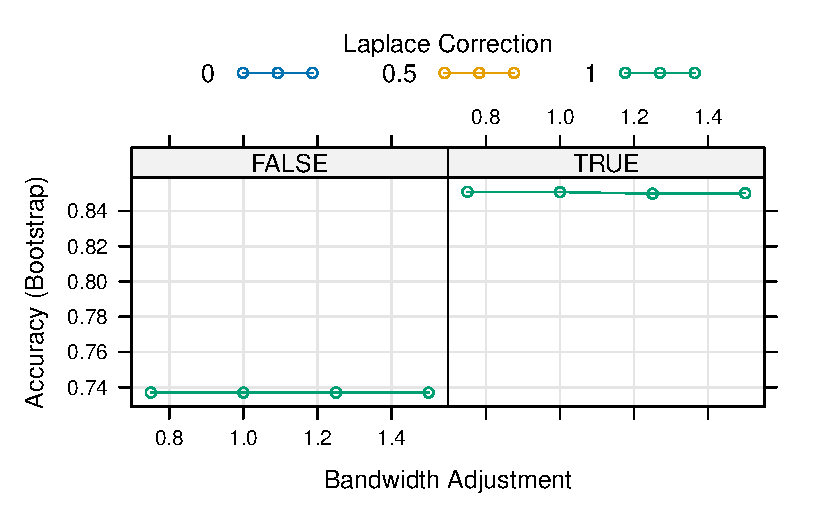
\includegraphics[keepaspectratio]{KnnNB_files/figure-pdf/nb_caret_parametrizar-1.pdf}}

\subsection{Python}

\begin{Shaded}
\begin{Highlighting}[]
\ImportTok{from}\NormalTok{ sklearn.model\_selection }\ImportTok{import}\NormalTok{ GridSearchCV, StratifiedKFold}
\ImportTok{from}\NormalTok{ sklearn.naive\_bayes }\ImportTok{import}\NormalTok{ MultinomialNB, BernoulliNB, ComplementNB}

\CommentTok{\# Métrica (elige la que te convenga)}
\NormalTok{scorer }\OperatorTok{=} \StringTok{"balanced\_accuracy"}  \CommentTok{\# o \textquotesingle{}balanced\_accuracy\textquotesingle{}, \textquotesingle{}roc\_auc\textquotesingle{}, \textquotesingle{}accuracy\textquotesingle{}, etc.}


\NormalTok{pipe }\OperatorTok{=}\NormalTok{ Pipeline([}
\NormalTok{    (}\StringTok{"clf"}\NormalTok{, MultinomialNB())  }\CommentTok{\# nombre del paso = \textquotesingle{}clf\textquotesingle{}}
\NormalTok{])}

\CommentTok{\# Espacio de búsqueda: probamos 3 NB distintos}
\NormalTok{param\_grid }\OperatorTok{=}\NormalTok{ [}
\NormalTok{  \{  }\CommentTok{\# MultinomialNB}
    \StringTok{"clf"}\NormalTok{: [MultinomialNB()],}
    \StringTok{"clf\_\_alpha"}\NormalTok{: [}\FloatTok{1e{-}3}\NormalTok{, }\FloatTok{1e{-}2}\NormalTok{, }\FloatTok{1e{-}1}\NormalTok{, }\FloatTok{1.0}\NormalTok{, }\FloatTok{2.0}\NormalTok{],}
    \StringTok{"clf\_\_fit\_prior"}\NormalTok{: [}\VariableTok{True}\NormalTok{, }\VariableTok{False}\NormalTok{],}
\NormalTok{  \},}
\NormalTok{  \{  }\CommentTok{\# ComplementNB}
    \StringTok{"clf"}\NormalTok{: [ComplementNB()],}
    \StringTok{"clf\_\_alpha"}\NormalTok{: [}\FloatTok{1e{-}3}\NormalTok{, }\FloatTok{1e{-}2}\NormalTok{, }\FloatTok{1e{-}1}\NormalTok{, }\FloatTok{1.0}\NormalTok{, }\FloatTok{2.0}\NormalTok{],}
    \StringTok{"clf\_\_fit\_prior"}\NormalTok{: [}\VariableTok{True}\NormalTok{, }\VariableTok{False}\NormalTok{],}
    \StringTok{"clf\_\_norm"}\NormalTok{: [}\VariableTok{True}\NormalTok{, }\VariableTok{False}\NormalTok{],}
\NormalTok{  \},}
\NormalTok{  \{  }\CommentTok{\# BernoulliNB}
    \StringTok{"clf"}\NormalTok{: [BernoulliNB()],}
    \StringTok{"clf\_\_alpha"}\NormalTok{: [}\FloatTok{1e{-}3}\NormalTok{, }\FloatTok{1e{-}2}\NormalTok{, }\FloatTok{1e{-}1}\NormalTok{, }\FloatTok{1.0}\NormalTok{, }\FloatTok{2.0}\NormalTok{],}
\NormalTok{  \},}
\NormalTok{]}

\NormalTok{cv }\OperatorTok{=}\NormalTok{ StratifiedKFold(n\_splits}\OperatorTok{=}\DecValTok{5}\NormalTok{, shuffle}\OperatorTok{=}\VariableTok{True}\NormalTok{, random\_state}\OperatorTok{=}\DecValTok{42}\NormalTok{)}

\NormalTok{grid }\OperatorTok{=}\NormalTok{ GridSearchCV(}
\NormalTok{    estimator}\OperatorTok{=}\NormalTok{pipe,}
\NormalTok{    param\_grid}\OperatorTok{=}\NormalTok{param\_grid,}
\NormalTok{    scoring}\OperatorTok{=}\StringTok{"roc\_auc"}\NormalTok{,}
\NormalTok{    cv}\OperatorTok{=}\NormalTok{cv,}
\NormalTok{    n\_jobs}\OperatorTok{=}\DecValTok{1}\NormalTok{,     }\CommentTok{\# importante en tu entorno}
\NormalTok{    refit}\OperatorTok{=}\VariableTok{True}\NormalTok{,}
\NormalTok{    verbose}\OperatorTok{=}\DecValTok{1}
\NormalTok{)}

\NormalTok{grid.fit(X\_train\_df, y\_trainPy)}
\end{Highlighting}
\end{Shaded}

\begin{verbatim}
Fitting 5 folds for each of 35 candidates, totalling 175 fits
GridSearchCV(cv=StratifiedKFold(n_splits=5, random_state=42, shuffle=True),
             estimator=Pipeline(steps=[('clf', MultinomialNB())]), n_jobs=1,
             param_grid=[{'clf': [MultinomialNB()],
                          'clf__alpha': [0.001, 0.01, 0.1, 1.0, 2.0],
                          'clf__fit_prior': [True, False]},
                         {'clf': [ComplementNB()],
                          'clf__alpha': [0.001, 0.01, 0.1, 1.0, 2.0],
                          'clf__fit_prior': [True, False],
                          'clf__norm': [True, False]},
                         {'clf': [BernoulliNB()],
                          'clf__alpha': [0.001, 0.01, 0.1, 1.0, 2.0]}],
             scoring='roc_auc', verbose=1)
\end{verbatim}

\begin{Shaded}
\begin{Highlighting}[]
\BuiltInTok{print}\NormalTok{(}\StringTok{"Best:"}\NormalTok{, grid.best\_estimator\_)}
\end{Highlighting}
\end{Shaded}

\begin{verbatim}
Best: Pipeline(steps=[('clf', ComplementNB(alpha=2.0, norm=True))])
\end{verbatim}

\begin{Shaded}
\begin{Highlighting}[]
\BuiltInTok{print}\NormalTok{(}\StringTok{"Params:"}\NormalTok{, grid.best\_params\_)}
\end{Highlighting}
\end{Shaded}

\begin{verbatim}
Params: {'clf': ComplementNB(), 'clf__alpha': 2.0, 'clf__fit_prior': True, 'clf__norm': True}
\end{verbatim}

\begin{Shaded}
\begin{Highlighting}[]
\BuiltInTok{print}\NormalTok{(}\StringTok{"CV score:"}\NormalTok{, grid.best\_score\_)}
\end{Highlighting}
\end{Shaded}

\begin{verbatim}
CV score: 0.7211343106077495
\end{verbatim}

\subsubsection{Predicción de la variable
respuesta}\label{predicciuxf3n-de-la-variable-respuesta-2}

\subsection{R: R base}

\begin{Shaded}
\begin{Highlighting}[]
\FunctionTok{head}\NormalTok{(}\FunctionTok{predict}\NormalTok{(nb\_base, X\_test, }\AttributeTok{type =} \StringTok{"class"}\NormalTok{))}
\end{Highlighting}
\end{Shaded}

\begin{verbatim}
[1] Yes No  No  No  Yes No 
Levels: No Yes
\end{verbatim}

\begin{Shaded}
\begin{Highlighting}[]
\FunctionTok{head}\NormalTok{(}\FunctionTok{predict}\NormalTok{(nb\_base, X\_test, }\AttributeTok{type =} \StringTok{"raw"}\NormalTok{))}
\end{Highlighting}
\end{Shaded}

\begin{verbatim}
               No        Yes
[1,] 2.226092e-01 0.77739080
[2,] 5.937698e-01 0.40623023
[3,] 6.046064e-01 0.39539356
[4,] 9.384762e-01 0.06152378
[5,] 3.985234e-05 0.99996015
[6,] 8.472974e-01 0.15270257
\end{verbatim}

\subsection{\texorpdfstring{R: Packages
\texttt{caret}}{R: Packages caret}}

\begin{Shaded}
\begin{Highlighting}[]
\FunctionTok{head}\NormalTok{(}\FunctionTok{predict}\NormalTok{(naive\_bayes\_via\_caret2, X\_testC))}
\FunctionTok{head}\NormalTok{(}\FunctionTok{predict}\NormalTok{(naive\_bayes\_via\_caret2, X\_testC, }\AttributeTok{type =} \StringTok{"prob"}\NormalTok{))}
\end{Highlighting}
\end{Shaded}

\subsection{Python}

\begin{Shaded}
\begin{Highlighting}[]
\ImportTok{from}\NormalTok{ sklearn.metrics }\ImportTok{import}\NormalTok{ confusion\_matrix, balanced\_accuracy\_score}

\CommentTok{\# Make predictions}
\NormalTok{train\_predict }\OperatorTok{=}\NormalTok{ naive\_bayes\_fit.predict(X\_train\_df)}
\NormalTok{test\_predict }\OperatorTok{=}\NormalTok{ naive\_bayes\_fit.predict(X\_test\_df)}

\KeywordTok{def}\NormalTok{ get\_scores(y\_real, predict):}
\NormalTok{  ba\_train }\OperatorTok{=}\NormalTok{ balanced\_accuracy\_score(y\_real, predict)}
\NormalTok{  cm\_train }\OperatorTok{=}\NormalTok{ confusion\_matrix(y\_real, predict)}

  \ControlFlowTok{return}\NormalTok{ ba\_train, cm\_train }

\KeywordTok{def}\NormalTok{ print\_scores(scores):}
  \ControlFlowTok{return} \SpecialStringTok{f"Balanced Accuracy: }\SpecialCharTok{\{}\NormalTok{scores[}\DecValTok{0}\NormalTok{]}\SpecialCharTok{\}}\CharTok{\textbackslash{}n}\SpecialStringTok{Confussion Matrix:}\CharTok{\textbackslash{}n}\SpecialStringTok{ }\SpecialCharTok{\{}\NormalTok{scores[}\DecValTok{1}\NormalTok{]}\SpecialCharTok{\}}\SpecialStringTok{"}

\NormalTok{train\_scores }\OperatorTok{=}\NormalTok{ get\_scores(y\_trainPy, train\_predict)}
\NormalTok{test\_scores }\OperatorTok{=}\NormalTok{ get\_scores(y\_testPy, test\_predict)}


\BuiltInTok{print}\NormalTok{(}\StringTok{"\#\# Train Scores"}\NormalTok{)}
\end{Highlighting}
\end{Shaded}

\begin{verbatim}
## Train Scores
\end{verbatim}

\begin{Shaded}
\begin{Highlighting}[]
\BuiltInTok{print}\NormalTok{(print\_scores(train\_scores))}
\end{Highlighting}
\end{Shaded}

\begin{verbatim}
Balanced Accuracy: 0.6493724679513846
Confussion Matrix:
 [[966 347]
 [104 134]]
\end{verbatim}

\begin{Shaded}
\begin{Highlighting}[]
\BuiltInTok{print}\NormalTok{(}\StringTok{"}\CharTok{\textbackslash{}n\textbackslash{}n}\StringTok{\#\# Test Scores"}\NormalTok{)}
\end{Highlighting}
\end{Shaded}

\begin{verbatim}


## Test Scores
\end{verbatim}

\begin{Shaded}
\begin{Highlighting}[]
\BuiltInTok{print}\NormalTok{(print\_scores(test\_scores))}
\end{Highlighting}
\end{Shaded}

\begin{verbatim}
Balanced Accuracy: 0.6157894736842106
Confussion Matrix:
 [[432 138]
 [ 50  45]]
\end{verbatim}

\subsubsection{\texorpdfstring{Validación de la \emph{performance} del
modelo}{Validación de la performance del modelo}}\label{validaciuxf3n-de-la-performance-del-modelo-1}

\subsection{R: R base}

\begin{Shaded}
\begin{Highlighting}[]
\NormalTok{nb\_trn\_pred }\OtherTok{=} \FunctionTok{predict}\NormalTok{(nb\_base, X\_train)}
\NormalTok{nb\_tst\_pred }\OtherTok{=} \FunctionTok{predict}\NormalTok{(nb\_base, X\_test)}
\end{Highlighting}
\end{Shaded}

\begin{Shaded}
\begin{Highlighting}[]
\FunctionTok{calc\_class\_err}\NormalTok{(}\AttributeTok{predicted =}\NormalTok{ nb\_trn\_pred, }\AttributeTok{actual =}\NormalTok{ y\_train)}
\end{Highlighting}
\end{Shaded}

\begin{verbatim}
[1] 1
\end{verbatim}

\begin{Shaded}
\begin{Highlighting}[]
\FunctionTok{calc\_class\_err}\NormalTok{(}\AttributeTok{predicted =}\NormalTok{ nb\_tst\_pred, }\AttributeTok{actual =}\NormalTok{ y\_test)}
\end{Highlighting}
\end{Shaded}

\begin{verbatim}
[1] 1
\end{verbatim}

\begin{Shaded}
\begin{Highlighting}[]
\FunctionTok{table}\NormalTok{(}\AttributeTok{predicted =}\NormalTok{ nb\_tst\_pred, }\AttributeTok{actual =}\NormalTok{ y\_test)}
\end{Highlighting}
\end{Shaded}

\begin{verbatim}
         actual
predicted 30 31 32 33 34 35 36 37 38 39 40 41 42 43 44 45 46 47 48 49 50 51 52
      No   0  0  0  3  1  4  4  4  3  9  6  4  6  6 11  3 13 18 11 21 15 15 15
      Yes  1  1  2  2  3  4  3  1  4  2  2  3  6  5  3  5  1  5  5  9 12  7  6
         actual
predicted 53 54 55 56 57 58 59 60 61 62 63 64 65 66 67 68 69 70 71 72 73 74 75
      No  18 20 18 15  9  8  8 12  6  6 13  7  8  7  5  8 10 10  7  6  7  8  2
      Yes 11  9  5  6  7  3  8  8 10  5  9  3  4  7  4  5 11  7 11  3  8  5  3
         actual
predicted 76 77 78 79 80 81 82 84 125
      No   3  1  1  3  0  0  0  0   0
      Yes  6  2  3  1  3  3  3  1   1
\end{verbatim}

\begin{Shaded}
\begin{Highlighting}[]
\FunctionTok{library}\NormalTok{(e1071)}
\FunctionTok{library}\NormalTok{(ggplot2)}

\NormalTok{y\_train }\OtherTok{\textless{}{-}} \FunctionTok{factor}\NormalTok{(y\_train)}
\NormalTok{y\_test  }\OtherTok{\textless{}{-}} \FunctionTok{factor}\NormalTok{(y\_test, }\AttributeTok{levels =} \FunctionTok{levels}\NormalTok{(y\_train))}

\CommentTok{\# 1) Pasar predictores a numérico con dummies (model.matrix)}
\CommentTok{\#    Si X\_* ya NO incluyen la respuesta, usa \textasciitilde{} . {-} 1}
\NormalTok{mm\_train }\OtherTok{\textless{}{-}} \FunctionTok{model.matrix}\NormalTok{(}\SpecialCharTok{\textasciitilde{}}\NormalTok{ . }\SpecialCharTok{{-}} \DecValTok{1}\NormalTok{, }\AttributeTok{data =}\NormalTok{ X\_train)  }\CommentTok{\# matriz numérica}
\NormalTok{mm\_test  }\OtherTok{\textless{}{-}} \FunctionTok{model.matrix}\NormalTok{(}\SpecialCharTok{\textasciitilde{}}\NormalTok{ . }\SpecialCharTok{{-}} \DecValTok{1}\NormalTok{, }\AttributeTok{data =}\NormalTok{ X\_test)}

\CommentTok{\# 2) PCA en TRAIN (centrado y escalado), proyectar }\AlertTok{TEST}
\NormalTok{pca }\OtherTok{\textless{}{-}} \FunctionTok{prcomp}\NormalTok{(mm\_train, }\AttributeTok{center =} \ConstantTok{TRUE}\NormalTok{, }\AttributeTok{scale. =} \ConstantTok{TRUE}\NormalTok{)}
\NormalTok{Z\_train }\OtherTok{\textless{}{-}} \FunctionTok{predict}\NormalTok{(pca, }\AttributeTok{newdata =}\NormalTok{ mm\_train)[, }\DecValTok{1}\SpecialCharTok{:}\DecValTok{2}\NormalTok{]}
\NormalTok{Z\_test  }\OtherTok{\textless{}{-}} \FunctionTok{predict}\NormalTok{(pca, }\AttributeTok{newdata =}\NormalTok{ mm\_test)[, }\DecValTok{1}\SpecialCharTok{:}\DecValTok{2}\NormalTok{]}
\FunctionTok{colnames}\NormalTok{(Z\_train) }\OtherTok{\textless{}{-}} \FunctionTok{c}\NormalTok{(}\StringTok{"PC1"}\NormalTok{,}\StringTok{"PC2"}\NormalTok{)}
\FunctionTok{colnames}\NormalTok{(Z\_test)  }\OtherTok{\textless{}{-}} \FunctionTok{c}\NormalTok{(}\StringTok{"PC1"}\NormalTok{,}\StringTok{"PC2"}\NormalTok{)}

\CommentTok{\# 3) Naive Bayes (e1071) en el plano PCA}
\NormalTok{nb }\OtherTok{\textless{}{-}} \FunctionTok{naiveBayes}\NormalTok{(}\AttributeTok{x =} \FunctionTok{as.data.frame}\NormalTok{(Z\_train), }\AttributeTok{y =}\NormalTok{ y\_train, }\AttributeTok{laplace =} \DecValTok{0}\NormalTok{)}

\CommentTok{\# 4) Grid y predicción para pintar la frontera}
\NormalTok{h }\OtherTok{\textless{}{-}} \FloatTok{0.02}
\NormalTok{x\_min }\OtherTok{\textless{}{-}} \FunctionTok{min}\NormalTok{(Z\_train[,}\DecValTok{1}\NormalTok{]) }\SpecialCharTok{{-}} \DecValTok{1}\NormalTok{; x\_max }\OtherTok{\textless{}{-}} \FunctionTok{max}\NormalTok{(Z\_train[,}\DecValTok{1}\NormalTok{]) }\SpecialCharTok{+} \DecValTok{1}
\NormalTok{y\_min }\OtherTok{\textless{}{-}} \FunctionTok{min}\NormalTok{(Z\_train[,}\DecValTok{2}\NormalTok{]) }\SpecialCharTok{{-}} \DecValTok{1}\NormalTok{; y\_max }\OtherTok{\textless{}{-}} \FunctionTok{max}\NormalTok{(Z\_train[,}\DecValTok{2}\NormalTok{]) }\SpecialCharTok{+} \DecValTok{1}
\NormalTok{grid }\OtherTok{\textless{}{-}} \FunctionTok{expand.grid}\NormalTok{(}\AttributeTok{PC1 =} \FunctionTok{seq}\NormalTok{(x\_min, x\_max, }\AttributeTok{by =}\NormalTok{ h),}
                    \AttributeTok{PC2 =} \FunctionTok{seq}\NormalTok{(y\_min, y\_max, }\AttributeTok{by =}\NormalTok{ h))}
\NormalTok{grid}\SpecialCharTok{$}\NormalTok{pred }\OtherTok{\textless{}{-}} \FunctionTok{predict}\NormalTok{(nb, }\AttributeTok{newdata =}\NormalTok{ grid)}

\CommentTok{\# 5) Plot fondo + puntos}
\NormalTok{pal\_fill }\OtherTok{\textless{}{-}} \FunctionTok{c}\NormalTok{(}\StringTok{"No"} \OtherTok{=} \StringTok{"\#FFAAAA"}\NormalTok{, }\StringTok{"Yes"} \OtherTok{=} \StringTok{"\#b3ffff"}\NormalTok{)}
\NormalTok{pal\_pts  }\OtherTok{\textless{}{-}} \FunctionTok{c}\NormalTok{(}\StringTok{"No"} \OtherTok{=} \StringTok{"\#FF0000"}\NormalTok{, }\StringTok{"Yes"} \OtherTok{=} \StringTok{"\#00ffff"}\NormalTok{)}

\NormalTok{df\_train }\OtherTok{\textless{}{-}} \FunctionTok{data.frame}\NormalTok{(Z\_train, }\AttributeTok{clase =}\NormalTok{ y\_train, }\AttributeTok{split =} \StringTok{"Train"}\NormalTok{)}
\NormalTok{df\_test  }\OtherTok{\textless{}{-}} \FunctionTok{data.frame}\NormalTok{(Z\_test,  }\AttributeTok{clase =}\NormalTok{ y\_test,  }\AttributeTok{split =} \StringTok{"Test"}\NormalTok{)}

\FunctionTok{ggplot}\NormalTok{() }\SpecialCharTok{+}
  \FunctionTok{geom\_raster}\NormalTok{(}\AttributeTok{data =}\NormalTok{ grid, }\FunctionTok{aes}\NormalTok{(PC1, PC2, }\AttributeTok{fill =}\NormalTok{ pred)) }\SpecialCharTok{+}
  \FunctionTok{scale\_fill\_manual}\NormalTok{(}\AttributeTok{values =}\NormalTok{ pal\_fill, }\AttributeTok{name =} \StringTok{"Fondo"}\NormalTok{) }\SpecialCharTok{+}
  \FunctionTok{geom\_point}\NormalTok{(}\AttributeTok{data =}\NormalTok{ df\_train, }\FunctionTok{aes}\NormalTok{(PC1, PC2, }\AttributeTok{color =}\NormalTok{ clase), }\AttributeTok{size =} \FloatTok{1.8}\NormalTok{) }\SpecialCharTok{+}
  \FunctionTok{geom\_point}\NormalTok{(}\AttributeTok{data =}\NormalTok{ df\_test,  }\FunctionTok{aes}\NormalTok{(PC1, PC2, }\AttributeTok{color =}\NormalTok{ clase), }\AttributeTok{size =} \FloatTok{2.2}\NormalTok{, }\AttributeTok{shape =} \DecValTok{21}\NormalTok{) }\SpecialCharTok{+}
  \FunctionTok{scale\_color\_manual}\NormalTok{(}\AttributeTok{values =}\NormalTok{ pal\_pts, }\AttributeTok{name =} \StringTok{"Puntos"}\NormalTok{) }\SpecialCharTok{+}
  \FunctionTok{coord\_equal}\NormalTok{(}\AttributeTok{expand =} \ConstantTok{FALSE}\NormalTok{, }\AttributeTok{xlim =} \FunctionTok{c}\NormalTok{(x\_min, x\_max), }\AttributeTok{ylim =} \FunctionTok{c}\NormalTok{(y\_min, y\_max)) }\SpecialCharTok{+}
  \FunctionTok{labs}\NormalTok{(}\AttributeTok{title =} \StringTok{"Frontera Naive Bayes (e1071) en plano PCA"}\NormalTok{, }\AttributeTok{x =} \StringTok{"PC1"}\NormalTok{, }\AttributeTok{y =} \StringTok{"PC2"}\NormalTok{) }\SpecialCharTok{+}
  \FunctionTok{theme\_minimal}\NormalTok{()}
\end{Highlighting}
\end{Shaded}

\subsection{\texorpdfstring{R: Packages
\texttt{caret}}{R: Packages caret}}

\begin{Shaded}
\begin{Highlighting}[]
\FunctionTok{confusionMatrix}\NormalTok{(naive\_bayes\_via\_caret2)}
\end{Highlighting}
\end{Shaded}

\begin{verbatim}
Bootstrapped (25 reps) Confusion Matrix 

(entries are percentual average cell counts across resamples)
 
          Reference
Prediction   No  Yes
       No  84.1 14.1
       Yes  0.9  1.0
                            
 Accuracy (average) : 0.8509
\end{verbatim}

\begin{Shaded}
\begin{Highlighting}[]
\FunctionTok{ggplot}\NormalTok{(}\FunctionTok{melt}\NormalTok{(naive\_bayes\_via\_caret2}\SpecialCharTok{$}\NormalTok{resample[,}\SpecialCharTok{{-}}\DecValTok{4}\NormalTok{]), }\FunctionTok{aes}\NormalTok{(}\AttributeTok{x =}\NormalTok{ variable, }\AttributeTok{y =}\NormalTok{ value, }\AttributeTok{fill=}\NormalTok{variable)) }\SpecialCharTok{+}
  \FunctionTok{geom\_boxplot}\NormalTok{(}\AttributeTok{show.legend=}\ConstantTok{FALSE}\NormalTok{) }\SpecialCharTok{+}
  \FunctionTok{xlab}\NormalTok{(}\ConstantTok{NULL}\NormalTok{) }\SpecialCharTok{+} \FunctionTok{ylab}\NormalTok{(}\ConstantTok{NULL}\NormalTok{)}
\end{Highlighting}
\end{Shaded}

\pandocbounded{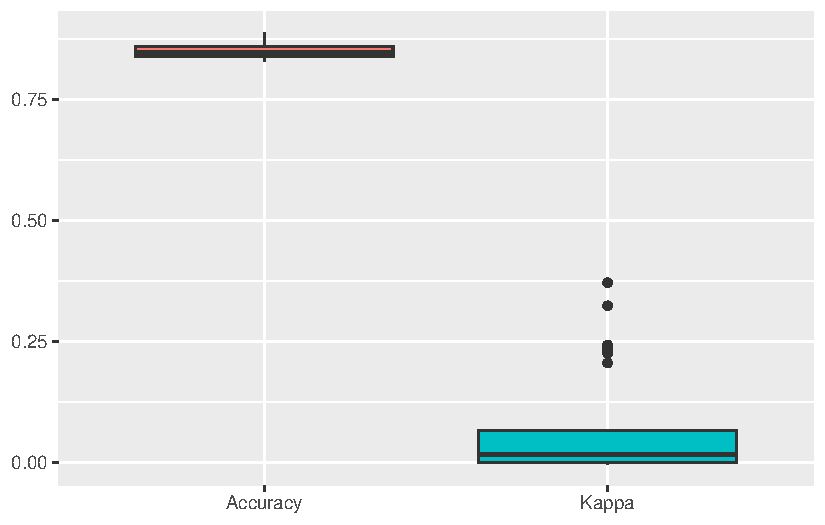
\includegraphics[keepaspectratio]{KnnNB_files/figure-pdf/unnamed-chunk-7-1.pdf}}

\begin{Shaded}
\begin{Highlighting}[]
\FunctionTok{library}\NormalTok{(caret)}
\FunctionTok{library}\NormalTok{(ggplot2)}
\FunctionTok{set.seed}\NormalTok{(}\DecValTok{123}\NormalTok{)}

\CommentTok{\# y como factor}
\NormalTok{y\_trainC }\OtherTok{\textless{}{-}} \FunctionTok{factor}\NormalTok{(y\_trainC)}
\NormalTok{y\_testC  }\OtherTok{\textless{}{-}} \FunctionTok{factor}\NormalTok{(y\_testC, }\AttributeTok{levels =} \FunctionTok{levels}\NormalTok{(y\_train))}

\CommentTok{\# 1) Preprocesado: centrar, escalar, PCA=2 (ajustado en train)}
\NormalTok{preproc }\OtherTok{\textless{}{-}} \FunctionTok{preProcess}\NormalTok{(X\_trainC, }\AttributeTok{method =} \FunctionTok{c}\NormalTok{(}\StringTok{"center"}\NormalTok{, }\StringTok{"scale"}\NormalTok{, }\StringTok{"pca"}\NormalTok{), }\AttributeTok{pcaComp =} \DecValTok{2}\NormalTok{)}
\NormalTok{Z\_train }\OtherTok{\textless{}{-}} \FunctionTok{predict}\NormalTok{(preproc, X\_trainC)  }\CommentTok{\# PC1, PC2}
\NormalTok{Z\_test  }\OtherTok{\textless{}{-}} \FunctionTok{predict}\NormalTok{(preproc, X\_testC)}

\CommentTok{\# 2) Entrenar Naive Bayes (klaR) en el espacio PCA (dos predictores)}
\NormalTok{ctrl }\OtherTok{\textless{}{-}} \FunctionTok{trainControl}\NormalTok{(}\AttributeTok{method =} \StringTok{"cv"}\NormalTok{, }\AttributeTok{number =} \DecValTok{5}\NormalTok{, }\AttributeTok{classProbs =} \ConstantTok{TRUE}\NormalTok{,}
                     \AttributeTok{summaryFunction =}\NormalTok{ twoClassSummary)}
\NormalTok{modelo\_nb }\OtherTok{\textless{}{-}} \FunctionTok{train}\NormalTok{(}
  \AttributeTok{x =}\NormalTok{ Z\_train[, }\FunctionTok{c}\NormalTok{(}\StringTok{"PC1"}\NormalTok{, }\StringTok{"PC2"}\NormalTok{)], }\AttributeTok{y =}\NormalTok{ y\_trainC,}
  \AttributeTok{method =} \StringTok{"nb"}\NormalTok{,                 }\CommentTok{\# klaR::NaiveBayes vía caret}
  \AttributeTok{trControl =}\NormalTok{ ctrl,}
  \AttributeTok{metric =} \StringTok{"ROC"}\NormalTok{,                }\CommentTok{\# mejor que Accuracy si hay desbalance}
  \AttributeTok{tuneGrid =} \FunctionTok{expand.grid}\NormalTok{(}
    \AttributeTok{usekernel =} \FunctionTok{c}\NormalTok{(}\ConstantTok{TRUE}\NormalTok{, }\ConstantTok{FALSE}\NormalTok{),}
    \AttributeTok{fL =} \FunctionTok{c}\NormalTok{(}\DecValTok{0}\NormalTok{, }\DecValTok{1}\NormalTok{),                }\CommentTok{\# laplace}
    \AttributeTok{adjust =} \FunctionTok{c}\NormalTok{(}\DecValTok{1}\NormalTok{, }\DecValTok{2}\NormalTok{)}
\NormalTok{  )}
\NormalTok{)}

\CommentTok{\# 3) Grid en el plano PCA (rango del TRAIN)}
\NormalTok{h }\OtherTok{\textless{}{-}} \FloatTok{0.02}
\NormalTok{x\_min }\OtherTok{\textless{}{-}} \FunctionTok{min}\NormalTok{(Z\_train}\SpecialCharTok{$}\NormalTok{PC1) }\SpecialCharTok{{-}} \DecValTok{1}\NormalTok{; x\_max }\OtherTok{\textless{}{-}} \FunctionTok{max}\NormalTok{(Z\_train}\SpecialCharTok{$}\NormalTok{PC1) }\SpecialCharTok{+} \DecValTok{1}
\NormalTok{y\_min }\OtherTok{\textless{}{-}} \FunctionTok{min}\NormalTok{(Z\_train}\SpecialCharTok{$}\NormalTok{PC2) }\SpecialCharTok{{-}} \DecValTok{1}\NormalTok{; y\_max }\OtherTok{\textless{}{-}} \FunctionTok{max}\NormalTok{(Z\_train}\SpecialCharTok{$}\NormalTok{PC2) }\SpecialCharTok{+} \DecValTok{1}
\NormalTok{grid }\OtherTok{\textless{}{-}} \FunctionTok{expand.grid}\NormalTok{(}
  \AttributeTok{PC1 =} \FunctionTok{seq}\NormalTok{(x\_min, x\_max, }\AttributeTok{by =}\NormalTok{ h),}
  \AttributeTok{PC2 =} \FunctionTok{seq}\NormalTok{(y\_min, y\_max, }\AttributeTok{by =}\NormalTok{ h)}
\NormalTok{)}

\CommentTok{\# 4) Predicción del modelo en el grid}
\NormalTok{grid}\SpecialCharTok{$}\NormalTok{pred }\OtherTok{\textless{}{-}} \FunctionTok{predict}\NormalTok{(modelo\_nb, }\AttributeTok{newdata =}\NormalTok{ grid)}

\CommentTok{\# 5) Plot fondo + puntos}
\NormalTok{pal\_fill }\OtherTok{\textless{}{-}} \FunctionTok{c}\NormalTok{(}\StringTok{"No"} \OtherTok{=} \StringTok{"\#FFAAAA"}\NormalTok{, }\StringTok{"Yes"} \OtherTok{=} \StringTok{"\#b3ffff"}\NormalTok{)}
\NormalTok{pal\_pts  }\OtherTok{\textless{}{-}} \FunctionTok{c}\NormalTok{(}\StringTok{"No"} \OtherTok{=} \StringTok{"\#FF0000"}\NormalTok{, }\StringTok{"Yes"} \OtherTok{=} \StringTok{"\#00ffff"}\NormalTok{)}

\NormalTok{df\_train }\OtherTok{\textless{}{-}} \FunctionTok{data.frame}\NormalTok{(Z\_train, }\AttributeTok{clase =}\NormalTok{ y\_trainC, }\AttributeTok{split =} \StringTok{"Train"}\NormalTok{)}
\NormalTok{df\_test  }\OtherTok{\textless{}{-}} \FunctionTok{data.frame}\NormalTok{(Z\_test,  }\AttributeTok{clase =}\NormalTok{ y\_testC,  }\AttributeTok{split =} \StringTok{"Test"}\NormalTok{)}

\FunctionTok{ggplot}\NormalTok{() }\SpecialCharTok{+}
  \FunctionTok{geom\_raster}\NormalTok{(}\AttributeTok{data =}\NormalTok{ grid, }\FunctionTok{aes}\NormalTok{(PC1, PC2, }\AttributeTok{fill =}\NormalTok{ pred), }\AttributeTok{alpha =} \DecValTok{1}\NormalTok{) }\SpecialCharTok{+}
  \FunctionTok{scale\_fill\_manual}\NormalTok{(}\AttributeTok{values =}\NormalTok{ pal\_fill, }\AttributeTok{name =} \StringTok{"Fondo"}\NormalTok{) }\SpecialCharTok{+}
  \FunctionTok{geom\_point}\NormalTok{(}\AttributeTok{data =}\NormalTok{ df\_train, }\FunctionTok{aes}\NormalTok{(PC1, PC2, }\AttributeTok{color =}\NormalTok{ clase), }\AttributeTok{size =} \FloatTok{1.8}\NormalTok{) }\SpecialCharTok{+}
  \FunctionTok{geom\_point}\NormalTok{(}\AttributeTok{data =}\NormalTok{ df\_test,  }\FunctionTok{aes}\NormalTok{(PC1, PC2, }\AttributeTok{color =}\NormalTok{ clase), }\AttributeTok{size =} \FloatTok{2.2}\NormalTok{, }\AttributeTok{shape =} \DecValTok{21}\NormalTok{) }\SpecialCharTok{+}
  \FunctionTok{scale\_color\_manual}\NormalTok{(}\AttributeTok{values =}\NormalTok{ pal\_pts, }\AttributeTok{name =} \StringTok{"Puntos"}\NormalTok{) }\SpecialCharTok{+}
  \FunctionTok{coord\_equal}\NormalTok{(}\AttributeTok{expand =} \ConstantTok{FALSE}\NormalTok{, }\AttributeTok{xlim =} \FunctionTok{c}\NormalTok{(x\_min, x\_max), }\AttributeTok{ylim =} \FunctionTok{c}\NormalTok{(y\_min, y\_max)) }\SpecialCharTok{+}
  \FunctionTok{labs}\NormalTok{(}\AttributeTok{title =} \StringTok{"Frontera Naive Bayes (caret::nb) en plano PCA"}\NormalTok{,}
       \AttributeTok{x =} \StringTok{"PC1"}\NormalTok{, }\AttributeTok{y =} \StringTok{"PC2"}\NormalTok{) }\SpecialCharTok{+}
  \FunctionTok{theme\_minimal}\NormalTok{() }\SpecialCharTok{+}
  \FunctionTok{theme}\NormalTok{(}\AttributeTok{legend.position =} \StringTok{"right"}\NormalTok{)}
\end{Highlighting}
\end{Shaded}

\subsection{Python}

\begin{Shaded}
\begin{Highlighting}[]
\ImportTok{from}\NormalTok{ sklearn.metrics }\ImportTok{import}\NormalTok{ classification\_report}
\BuiltInTok{print}\NormalTok{(classification\_report(y\_testPy, test\_predict))}
\end{Highlighting}
\end{Shaded}

\begin{verbatim}
              precision    recall  f1-score   support

          No       0.90      0.76      0.82       570
         Yes       0.25      0.47      0.32        95

    accuracy                           0.72       665
   macro avg       0.57      0.62      0.57       665
weighted avg       0.80      0.72      0.75       665
\end{verbatim}

\begin{Shaded}
\begin{Highlighting}[]
\ImportTok{import}\NormalTok{ numpy }\ImportTok{as}\NormalTok{ np}
\ImportTok{import}\NormalTok{ matplotlib.pyplot }\ImportTok{as}\NormalTok{ plt}
\ImportTok{from}\NormalTok{ matplotlib.colors }\ImportTok{import}\NormalTok{ ListedColormap}
\ImportTok{import}\NormalTok{ matplotlib.patches }\ImportTok{as}\NormalTok{ mpatches}

\ImportTok{from}\NormalTok{ sklearn.preprocessing }\ImportTok{import}\NormalTok{ StandardScaler, LabelEncoder}
\ImportTok{from}\NormalTok{ sklearn.decomposition }\ImportTok{import}\NormalTok{ PCA}
\ImportTok{from}\NormalTok{ sklearn.naive\_bayes }\ImportTok{import}\NormalTok{ GaussianNB  }\CommentTok{\# \textless{}\textless{} cambio clave}

\CommentTok{\# ==== Parámetros ====}
\NormalTok{h }\OperatorTok{=} \FloatTok{0.02}

\CommentTok{\# ==== 0) Tipos correctos ====}
\NormalTok{X\_trainPy }\OperatorTok{=}\NormalTok{ np.asarray(X\_trainPy, dtype}\OperatorTok{=}\BuiltInTok{float}\NormalTok{)}
\NormalTok{X\_testPy  }\OperatorTok{=}\NormalTok{ np.asarray(X\_testPy,  dtype}\OperatorTok{=}\BuiltInTok{float}\NormalTok{)}
\NormalTok{y\_trainPy }\OperatorTok{=}\NormalTok{ np.asarray(y\_trainPy)}
\NormalTok{y\_testPy  }\OperatorTok{=}\NormalTok{ np.asarray(y\_testPy)}

\CommentTok{\# Codificar etiquetas (para colorear y leyendas)}
\NormalTok{le }\OperatorTok{=}\NormalTok{ LabelEncoder()}
\NormalTok{y\_train\_num }\OperatorTok{=}\NormalTok{ le.fit\_transform(y\_trainPy)}
\NormalTok{y\_test\_num  }\OperatorTok{=}\NormalTok{ le.transform(y\_testPy)}

\CommentTok{\# ==== 1) Estandarizar (fit en train) + PCA (fit en train) ====}
\NormalTok{scaler }\OperatorTok{=}\NormalTok{ StandardScaler()}
\NormalTok{X\_train\_scaled }\OperatorTok{=}\NormalTok{ scaler.fit\_transform(X\_trainPy)}
\NormalTok{X\_test\_scaled  }\OperatorTok{=}\NormalTok{ scaler.transform(X\_testPy)}

\NormalTok{pca }\OperatorTok{=}\NormalTok{ PCA(n\_components}\OperatorTok{=}\DecValTok{2}\NormalTok{, random\_state}\OperatorTok{=}\DecValTok{0}\NormalTok{)}
\NormalTok{Z\_train }\OperatorTok{=}\NormalTok{ pca.fit\_transform(X\_train\_scaled).astype(}\BuiltInTok{float}\NormalTok{)}
\NormalTok{Z\_test  }\OperatorTok{=}\NormalTok{ pca.transform(X\_test\_scaled).astype(}\BuiltInTok{float}\NormalTok{)}

\CommentTok{\# ==== 2) Entrenar Naive Bayes (Gaussian) en el espacio PCA ====}
\NormalTok{clf }\OperatorTok{=}\NormalTok{ GaussianNB()}
\NormalTok{clf.fit(Z\_train, y\_train\_num)}
\end{Highlighting}
\end{Shaded}

\begin{verbatim}
GaussianNB()
\end{verbatim}

\begin{Shaded}
\begin{Highlighting}[]
\CommentTok{\# ==== 3) Mallado y predicción para el fondo ====}
\NormalTok{x\_min, x\_max }\OperatorTok{=}\NormalTok{ Z\_train[:, }\DecValTok{0}\NormalTok{].}\BuiltInTok{min}\NormalTok{() }\OperatorTok{{-}} \DecValTok{1}\NormalTok{, Z\_train[:, }\DecValTok{0}\NormalTok{].}\BuiltInTok{max}\NormalTok{() }\OperatorTok{+} \DecValTok{1}
\NormalTok{y\_min, y\_max }\OperatorTok{=}\NormalTok{ Z\_train[:, }\DecValTok{1}\NormalTok{].}\BuiltInTok{min}\NormalTok{() }\OperatorTok{{-}} \DecValTok{1}\NormalTok{, Z\_train[:, }\DecValTok{1}\NormalTok{].}\BuiltInTok{max}\NormalTok{() }\OperatorTok{+} \DecValTok{1}
\NormalTok{xx, yy }\OperatorTok{=}\NormalTok{ np.meshgrid(np.arange(x\_min, x\_max, h),}
\NormalTok{                     np.arange(y\_min, y\_max, h))}
\NormalTok{Z\_grid\_pred\_num }\OperatorTok{=}\NormalTok{ clf.predict(np.c\_[xx.ravel(), yy.ravel()]).reshape(xx.shape)}

\CommentTok{\# ==== 4) Paletas ====}
\NormalTok{cmap\_light }\OperatorTok{=}\NormalTok{ ListedColormap([}\StringTok{\textquotesingle{}\#FFAAAA\textquotesingle{}}\NormalTok{, }\StringTok{\textquotesingle{}\#b3ffff\textquotesingle{}}\NormalTok{])}
\NormalTok{cmap\_bold  }\OperatorTok{=}\NormalTok{ ListedColormap([}\StringTok{\textquotesingle{}\#FF0000\textquotesingle{}}\NormalTok{,  }\StringTok{\textquotesingle{}\#00ffff\textquotesingle{}}\NormalTok{])}

\CommentTok{\# ==== 5) Plot ====}
\NormalTok{plt.figure(figsize}\OperatorTok{=}\NormalTok{(}\DecValTok{7}\NormalTok{,}\DecValTok{5}\NormalTok{))}
\NormalTok{plt.pcolormesh(xx, yy, Z\_grid\_pred\_num, cmap}\OperatorTok{=}\NormalTok{cmap\_light, shading}\OperatorTok{=}\StringTok{\textquotesingle{}auto\textquotesingle{}}\NormalTok{)}

\NormalTok{plt.scatter(Z\_train[:, }\DecValTok{0}\NormalTok{], Z\_train[:, }\DecValTok{1}\NormalTok{], c}\OperatorTok{=}\NormalTok{y\_train\_num, cmap}\OperatorTok{=}\NormalTok{cmap\_bold,}
\NormalTok{            edgecolor}\OperatorTok{=}\StringTok{\textquotesingle{}k\textquotesingle{}}\NormalTok{, s}\OperatorTok{=}\DecValTok{25}\NormalTok{, alpha}\OperatorTok{=}\FloatTok{0.85}\NormalTok{, label}\OperatorTok{=}\StringTok{\textquotesingle{}Train\textquotesingle{}}\NormalTok{)}
\NormalTok{plt.scatter(Z\_test[:, }\DecValTok{0}\NormalTok{],  Z\_test[:, }\DecValTok{1}\NormalTok{],  c}\OperatorTok{=}\NormalTok{y\_test\_num,  cmap}\OperatorTok{=}\NormalTok{cmap\_bold,}
\NormalTok{            edgecolor}\OperatorTok{=}\StringTok{\textquotesingle{}k\textquotesingle{}}\NormalTok{, s}\OperatorTok{=}\DecValTok{35}\NormalTok{, marker}\OperatorTok{=}\StringTok{\textquotesingle{}o\textquotesingle{}}\NormalTok{, label}\OperatorTok{=}\StringTok{\textquotesingle{}Test\textquotesingle{}}\NormalTok{)}

\NormalTok{plt.xlim(xx.}\BuiltInTok{min}\NormalTok{(), xx.}\BuiltInTok{max}\NormalTok{())}\OperatorTok{;}\NormalTok{ plt.ylim(yy.}\BuiltInTok{min}\NormalTok{(), yy.}\BuiltInTok{max}\NormalTok{())}
\end{Highlighting}
\end{Shaded}

\begin{verbatim}
(-6.3391686872764605, 7.340831312723248)
(-4.7438491611385425, 5.696150838861235)
\end{verbatim}

\begin{Shaded}
\begin{Highlighting}[]
\NormalTok{plt.xlabel(}\StringTok{\textquotesingle{}PC1\textquotesingle{}}\NormalTok{)}\OperatorTok{;}\NormalTok{ plt.ylabel(}\StringTok{\textquotesingle{}PC2\textquotesingle{}}\NormalTok{)}
\NormalTok{plt.title(}\StringTok{"Frontera Naive Bayes (Gaussian) en plano PCA"}\NormalTok{)}

\CommentTok{\# Leyenda de clases (nombres originales)}
\NormalTok{classes }\OperatorTok{=} \BuiltInTok{list}\NormalTok{(le.classes\_)}
\NormalTok{palette }\OperatorTok{=}\NormalTok{ [}\StringTok{\textquotesingle{}\#FF0000\textquotesingle{}}\NormalTok{, }\StringTok{\textquotesingle{}\#00ffff\textquotesingle{}}\NormalTok{]}
\NormalTok{patches }\OperatorTok{=}\NormalTok{ [mpatches.Patch(color}\OperatorTok{=}\NormalTok{palette[i }\OperatorTok{\%} \BuiltInTok{len}\NormalTok{(palette)], label}\OperatorTok{=}\BuiltInTok{str}\NormalTok{(lbl))}
           \ControlFlowTok{for}\NormalTok{ i, lbl }\KeywordTok{in} \BuiltInTok{enumerate}\NormalTok{(classes)]}
\NormalTok{legend\_classes }\OperatorTok{=}\NormalTok{ plt.legend(handles}\OperatorTok{=}\NormalTok{patches, title}\OperatorTok{=}\StringTok{"Clases"}\NormalTok{,}
\NormalTok{                            loc}\OperatorTok{=}\StringTok{\textquotesingle{}upper right\textquotesingle{}}\NormalTok{, bbox\_to\_anchor}\OperatorTok{=}\NormalTok{(}\FloatTok{1.32}\NormalTok{, }\FloatTok{1.0}\NormalTok{))}
\NormalTok{plt.gca().add\_artist(legend\_classes)}

\NormalTok{plt.legend(loc}\OperatorTok{=}\StringTok{\textquotesingle{}best\textquotesingle{}}\NormalTok{)  }\CommentTok{\# Train/Test}
\NormalTok{plt.tight\_layout()}
\NormalTok{plt.show()}
\end{Highlighting}
\end{Shaded}

\pandocbounded{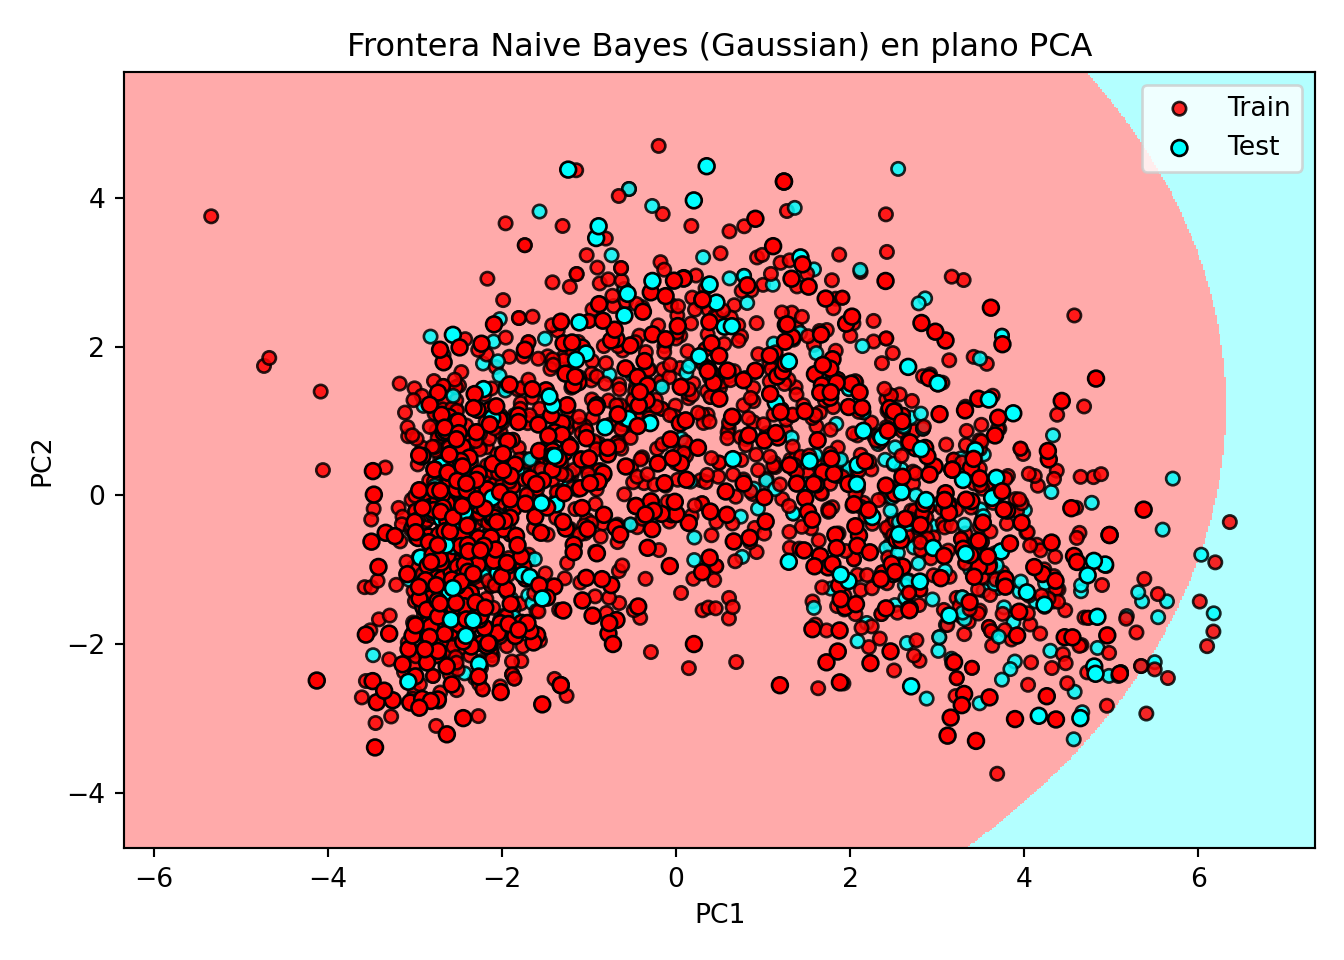
\includegraphics[keepaspectratio]{KnnNB_files/figure-pdf/grafico_clasificacion_python_nb-1.pdf}}

\subsection{Bibliografia}\label{bibliografia}

\begin{itemize}
\tightlist
\item
  https://daviddalpiaz.github.io/r
\item
\end{itemize}




\end{document}
